% Official ICML 2026 anonymous review style; vendor files are unmodified.
\documentclass{article}
\usepackage[T1]{fontenc}
\usepackage{microtype,graphicx,booktabs,tabularx,array}
\usepackage{amsmath,amssymb}
\usepackage{hyperref}
\usepackage{icml2026}
\usepackage{placeins}
\graphicspath{{figures/}}
\newcommand{\E}{\widehat{\mathcal E}}
\newcommand{\R}{\mathbb R}
\icmltitlerunning{Artist-Name Responses in Image Generation}
\hypersetup{pdfauthor={Anonymous},pdftitle={Artist-Name Responses beyond a Shared Painting Effect in Text-to-Image Generation}}
\begin{document}
\twocolumn[
\icmltitle{Artist-Name Responses beyond a Shared Painting Effect in Text-to-Image Generation}
\begin{icmlauthorlist}
\icmlauthor{Anonymous Authors}{anon}
\end{icmlauthorlist}
\icmlaffiliation{anon}{Anonymous Institution}
\icmlcorrespondingauthor{Anonymous Author}{anon.email@domain.com}
\icmlkeywords{text-to-image generation, evaluation, artist conditioning}
\vskip 0.3in
]
\printAffiliationsAndNotice{}
\begin{abstract}
Artist-name prompts can increase reference proximity without reproducing the
reference's painter differences. We audit 1,008 images from six requested
configurations, four painters, 14 scenes and two repeats, using 31 image
measurements, CLIP and a released CSD encoder. Common movement supplies
66.7--88.4\% of additional naming change beyond generic painting in the
31-feature metric and most learned prototype gain. A retrospective check on
2,000 separate SD-Turbo outputs with 25 matched-seed blocks finds 64.2\% common
change overall, but only 36.6\% in texture. Weak Monet--Sisley alignment in
five configurations' hand measurements becomes positive in both learned
representations. For prompted-name recovery, held-scene mean translation
changes accuracy while preserving centered painter contrasts. A further fixed
reference-calibrated abstention test lowers mean accepted error by 26.0 points
in its primary CSD setting, yet improves only 0.5 points over margin filtering
at equal coverage and omits some painters within configurations. These retrospective
analyses retain all configurations and adverse sensitivities. They show why
proximity, reference agreement and selective name recovery require different
checks; none validates perceived painter fidelity. The separate collection
reuses the historical target, and actual dependence in closed services remains
unidentified.
\end{abstract}
\section{Introduction}
An evaluator observes that images prompted ``in the style of Monet'' move
closer to Monet's reference collection. What should that observation establish?
A painting instruction can improve proximity to several related painters at
once. A classifier can recover prompted names from differences peculiar to a
generator. A high-confidence reference assignment can still identify the wrong
prompt. These possibilities require different evaluation checks.

Our main audit crosses six requested configurations with four related painters,
generic-painting and artist-free controls, 14 fixed scenes and two repeats
(1,008 images). A separate retained collection adds 2,000 SD-Turbo images under
a different template and 25 matched-seed blocks. We also test whether a rule
calibrated on historical artworks can withhold unreliable prompt-name assignments.
The targets are digital reference measurements and recorded prompt names.
Historical content and reproduction processes enter the finite reference target;
neither target establishes perceived resemblance. The additional analyses reuse
previously exposed data, with their new rules fixed before their outcomes.

The empirical question is how much an evaluation conclusion changes when its
target is made explicit. We separate common naming movement from labeled painter
contrasts, then separate reference-based decisions from within-generator label
structure. Common naming movement and a generated-to-reference mixture offset
are distinct: the first explains proximity gain over a prompt control, while
the second can change class intercepts without changing painter contrasts.
Table~\ref{tab:quantity-map} maps the required checks. These use established
geometry and decision rules; the contribution is the measured evaluation
behavior and its limits, not a new algorithm or perceptual metric.

\begin{table*}[t]
\caption{Evaluation questions and the checks needed to interpret their readouts.
All targets concern recorded images or prompt names, not perceptual fidelity.}
\label{tab:quantity-map}
\centering\small
\begin{tabularx}{\linewidth}{@{}p{.25\linewidth}p{.25\linewidth}X@{}}
\toprule
Question & Readout & Interpretation check\\\midrule
Does naming increase reference proximity? & Own-painter prototype gain & Separate common movement from labeled agreement.\\
Do painter differences match the reference? & Aligned amplitude $\beta$ and error $D$ & State the feature units, reference target and scene aggregation.\\
Can the prompt name be recovered? & Top-1 accuracy & Compare reference decisions, fixed mean translation and supervised generated centroids.\\
When should a name assignment be issued? & Accepted error and coverage & Test a fixed reference-calibrated gate against margin filtering at equal coverage.\\
\bottomrule
\end{tabularx}
\end{table*}


\section{Related Work}
\citet{somepalli2024style} introduce CSD and General Style Similarity: a generated
embedding's dot product with an averaged artist prototype, including
content-constrained prompts. \citet{su2025prompted} evaluate prompted-artist
recognition using content-controlled name substitutions and matched artist-free
images; generated-image retrieval usually outperforms real-image retrieval in
their benchmark. Our stronger generated-prototype comparator therefore
contextualizes an established domain distinction. We audit common and labeled
contributions to proximity gain, not a new recognition task.

\citet{frochte2026csd} diagnose raw CSD cosine and shared-tradition confusions,
then evaluate local-density readouts and input-resolution changes. Their
absolute-score and pair-verification study excludes closed-set discrimination.
Our controlled name interventions quantify common/labeled gain and connect a
separate mean offset to prompted-name decisions. The general warning that raw
style similarity needs validation is established, not our novelty claim.

\citet{deliege2025} assess stylistic imitation and stereotyping with experts.
AI-Pastiche studies authenticity and prompt adherence \citep{asperti2025pastiche};
AI-WikiArt uses painting-derived captions and vision-language models for
attribution \citep{fu2025aiwikiart}. Our measured painter contrasts and same-image
CLIP/CSD comparisons target neither convincing imitation nor physical authorship.

Quantitative art research examines color, composition and image statistics
\citep{kim2014,sigaki2018,lee2020}. Unlike the contextual image-to-image
experiments of \citet{kim2026}, our text-only intervention supplies no original
composition.

Generative evaluation separates fidelity and diversity \citep{naeem2020},
while conditional metrics distinguish within-condition variation from relationships
among means \citep{benny2021conditional}. We use independent-partition inner products
as the primary noise-corrected squared-difference estimator \citep{diedrichsen2017representational}
and energy statistics as a complementary distributional measure \citep{szekely2013}.
Processing sensitivity \citep{parmar2022} and limits of learned-embedding
separation \citep{asperti2026} motivate the source-quality checks and the
restriction to a specified digital reference target.

Target-domain centroid classifiers also address classifier bias under domain
shift \citep{liang2021atdoc}. Our retrospective decision diagnostic uses a fixed
mean translation and supervised centroids with frozen features; it is not an
adaptation-method contribution.
Selective classification trades prediction coverage for error
\citep{geifman2017selective}. We test a fixed reference-calibrated rejection rule;
distribution-shift guarantees require assumptions beyond those established for
these historical and generated panels \citep{tibshirani2019shift}.

\section{Design and Measurements}\label{sec:design}
\subsection{Painters and Reference Images}
The primary panel covers four related painters through 649 distinct reproductions: 297 Monet,
106 Sisley, 141 Pissarro and 105 C\'ezanne. Artist means receive equal weight,
so the larger Monet collection does not dominate the between-artist target.
A separate 221-work development panel sets common feature units; no primary
reference or generated image is used to fit that transformation. Both panels
were assembled before the present experiment and had been used in earlier
analyses. They are explicit, finite comparison panels rather than newly withheld
samples of each painter's complete oeuvre.

Reference files carry Wikimedia Commons source metadata and Wikidata work
identities \citep{commonsglam,vrandecic2014wikidata}. These support traceable
selection and rights records, but do not standardize photography, color
calibration or conservation state. These are measurements of digital
reproductions, whose capture conditions can affect the comparison.

\subsection{A Common-scene, Six-model Experiment}
We compare six requested service configurations, labeled GPT Image 1, GPT Image 2, GPT Image 2.5 Flare (Flare),
GPT Image 2.5 Sunburst (Sunburst), Nano Banana 2 and FLUX.2 Max (FLUX).
Fourteen fixed outdoor scene descriptions (briefs) span water,
built, land and mixed compositions. Each scene is crossed with six clauses:
no painting instruction; ``Render as an oil painting''; and ``Render as an oil
painting in the style of [painter]'' for each of the four painters. The scene
text is otherwise identical. Each model--scene--clause cell receives two
separately requested outputs, giving 1,008 images collected on 10 September 2026 (UTC).

All models receive text only and return 1,024-by-1,024-pixel images.
The four OpenAI requests specify medium quality; Nano Banana 2 specifies
1K resolution, while FLUX requests PNG output without an explicit resolution
field. These comparisons concern the recorded
configurations, not maximum attainable quality or equal expenditure per image.
Response records do not echo model identifiers, so these labels identify requested
configurations rather than independently verified checkpoints
(Appendix~\ref{app:provenance}).
The exact prompts, parameters and randomized request order were fixed before
collection. The 14 scenes are a fixed design,
not a random sample of all possible content.
Earlier, separate prompt interventions are summarized in Appendix~\ref{app:cohorts}.

Appendix Figure~\ref{fig:original-generated} shows all six conditions for one brief.
GPT Image 2's C\'ezanne trees have darker blue-green outlines than its Monet
and Sisley trees: a visible name response in this scene, whose agreement with
historical painter differences remains to be measured.



\subsection{What the Features Measure}\label{sec:features}
The 31 features in Table~\ref{tab:features} capture properties that need not
change together. Two images can have similar chroma (color strength) but different
hue diversity, or similar total contrast but different edge directions and
fine-scale texture. Such distinctions make results by feature family interpretable.
There are 11 color coordinates (lightness, chroma, hue and color increments),
eight spatial coordinates (spectra, gradients, orientations and quadrants),
and 12 texture coordinates (wavelet energy, local binary patterns and local contrast).
Correlated coordinates and sensitivity to image processing nevertheless prevent
treating Euclidean distance as a validated measure of artistic style.



Images undergo orientation correction and conversion to sRGB using valid
embedded profiles; compatible unprofiled files are treated as sRGB. The primary
pipeline preserves aspect ratio at a 512-pixel short side, using Lanczos resizing
without upsampling. No painting-region mask is applied: source margins or
calibration strips can enter the measurements. Each coordinate is centered and scaled by its
median and interquartile range in the development panel, with equal total
weight per painter. Thus a unit is a development-panel IQR in that coordinate,
not a perceptual just-noticeable difference. The Euclidean metric weights
standardized coordinates equally, without further equalizing feature families.



\section{Comparing Painter Differences}\label{sec:method}
\subsection{What Counts as Agreement?}\label{sec:contrast-intuition}
Subtract each set's four-painter mean to isolate labeled differences. For
example, reference Monet is $.325$ development-IQR units darker than Sisley
in median lightness; GPT Image 2's mean gap is $.254$ in that direction.
A shared brightness shift cannot create this contrast.
Aligned amplitude $\beta$ measures agreement along the reference pattern;
error $D$ also counts differences in other directions. No distinction, exact
agreement and doubled reference contrasts have expected errors 1, 0 and 1.
Thus stronger responses need not give lower error.

\subsection{Computing the Two Scores}
Let $\mu_a\in\R^{31}$ be painter $a$'s standardized reference mean and
$r_a=\mu_a-\frac14\sum_b\mu_b$ its contrast. The total squared size of these
contrasts, $H=\sum_a\|r_a\|^2$, normalizes both scores. Here $\|u\|^2$ sums squared
coordinates, $\langle u,v\rangle$ sums matching-coordinate products, and
hats mark estimates. For generated measurements $z_{msak}$, indices denote
model $m$, scene $s$, painter $a$ and repeat $k\in\{1,2\}$:
\begin{equation}
 d_{msak}=z_{msak}-\frac14\sum_b z_{msbk}.
 \label{eq:center}
\end{equation}
Centering removes shared additive shifts, but shared rescaling or mixing
of coordinates can still change the contrasts
(Appendix~\ref{app:score-details}). With $S=14$ scenes, the aligned response is
\begin{equation}
\begin{gathered}
\widehat\beta_{msk}=\frac{\sum_a\langle d_{msak},r_a\rangle}{H},\\
\widehat\beta_m=\frac1S\sum_s\frac{\widehat\beta_{ms1}+\widehat\beta_{ms2}}2.
\end{gathered}
\label{eq:beta}
\end{equation}
A positive value indicates an overall response along the reference differences;
it does not require agreement for each artist pair. Values above one indicate
exaggeration along that direction. To measure error, multiply the discrepancies
from the two repeats rather than squaring either repeat's discrepancy:
\begin{equation}
\begin{gathered}
\widehat D_{ms}=\frac1H\sum_a
\langle d_{msa1}-r_a,\ d_{msa2}-r_a\rangle,\\
\widehat D_m=\frac1S\sum_s\widehat D_{ms}.
\end{gathered}
\label{eq:distortion}
\end{equation}
Under stable conditional means and independent, mean-zero repeat errors,
noise that does not recur across requests contributes zero in expectation.
The expected score is then the normalized squared error of the scene-conditional
mean contrasts. Individual estimates can be negative; they are retained, not
interpreted as better-than-perfect recovery. The $D=1$ no-contrast benchmark
is a theoretical predictor, not the observed generic-painting arm.

Every scene is compared with the same pooled historical contrast. Scene-varying
artist responses therefore incur error even when their average matches that
target; this need not be an artistic mistake. We report both scene-wise error
and error after scene averaging (Appendix~\ref{app:score-details}).

\subsection{Model Comparisons and Uncertainty}
The prespecified 31-feature family contains six aligned responses and 15
model-pair error differences. Paired-scene Student intervals use a Bonferroni
adjustment for all 21, targeting approximate 95\% simultaneous coverage under
the stated model. Individual features, painters and outputs are not independent
replicates. Absolute-$D$ intervals are unadjusted descriptive summaries.

Inference conditions on the finite reference panel, scaling and 14 authored
briefs, assuming stable conditional means and independent scene/repeat error
blocks. Scene standard errors also include fixed scene heterogeneity and do
not isolate fresh-request variance. Two repeats cannot verify independence,
and the Student approximation guarantees neither actual service coverage nor
inference to unseen scenes. Under an assumed common trace correlation, the
Nano Banana 2--FLUX error point order crosses at $.251$
(Appendix~\ref{app:repeat-covariance}); actual dependence remains unidentified.
Declared scene, reference, feature-family and title-class sensitivities are
specified in Appendix~\ref{app:estimation}. They do not match compositions or
supply additional service observations.

\subsection{What the Additional Comparisons Test}\label{sec:diagnostics}
Artist-free and generic-painting arms characterize the removed common response.
Retrospective diagnostics examine all painter pairs, scenes and reference views.
A magnitude check fits one nonnegative multiplier of a model's centered
contrasts on 13 scenes and scores the omitted scene. It changes feature
contrasts, not images or references. These diagnostics do not expand the
confirmatory family (Appendix~\ref{app:diagnostics}).

\section{Results}\label{sec:results}
\subsection{A Response in the Right Direction Can Still Miss the Target}
All 1,008 outputs yield valid measurements. Every configuration's aligned-response
interval lies above zero under the stated inference model (Appendix
Table~\ref{tab:specificity-models}), but positive alignment need not give low error.
GPT Image 2 nearly matches the reference strength,
$\beta=.999\;[.893,1.104]$, while total error is $D=1.226$.
FLUX has lower alignment ($.470$) and the lowest error estimate ($.801$).
Only Flare--FLUX and Sunburst--FLUX resolve positive error differences after
the 21-comparison adjustment; the other 13 intervals include zero.
No configuration is established to beat the no-contrast error benchmark of one.
These are full-frame comparisons; source correction changes which differences
are resolved (Section~\ref{sec:source-correction}).

\subsection{Most Scene-averaged Change Is Common to the Painter Names}\label{sec:shared-change}
After averaging scenes, named-minus-artist-free shifts comprise a four-name mean
and painter-specific departures. The mean includes the oil-painting clause and
any common naming response: 82.5--95.7\% of repeat-corrected squared change
(Table~\ref{tab:shared-change}). Retrospectively changing the baseline to generic
oil painting isolates the additional naming change: 66.7--88.4\% is shared.
The painter-specific component is unchanged. Deleting each scene and recomputing
the ratios gives 65.9--90.2\% across models; these are sensitivity ranges,
not confidence intervals (Appendix~\ref{app:direct-naming}).

\begin{table*}[htbp]
\caption{Scene-averaged, repeat-corrected change. Shared is the four-name mean shift; between-name is departure from it. The artist-free baseline includes the painting clause; the retrospective generic-baseline row isolates additional naming. The last two rows compare the shared named-minus-free shift with generic-minus-free: corrected cosine measures directional agreement, and the ratio divides their corrected squared magnitudes, shared by generic.}
\label{tab:shared-change}
\centering\small\setlength{\tabcolsep}{3pt}
\begin{tabularx}{\linewidth}{@{}l*{6}{>{\centering\arraybackslash}X}@{}}
\toprule
& \shortstack{GPT Image\\1} & \shortstack{GPT Image\\2} & Flare & Sunburst & \shortstack{Nano\\Banana 2} & \shortstack{FLUX.2\\Max}\\\midrule
Free baseline: shared (\%) & 82.5 & 85.8 & 84.8 & 83.9 & 88.1 & 95.7\\
Free baseline: between-name (\%) & 17.5 & 14.2 & 15.2 & 16.1 & 11.9 & 4.3\\
Generic baseline: shared (\%) & 71.3 & 70.9 & 71.1 & 66.7 & 69.1 & 88.4\\
\midrule
Corrected cosine & 0.689 & 0.774 & 0.766 & 0.837 & 0.930 & 0.916\\
Squared-size ratio & 1.986 & 1.960 & 2.816 & 3.356 & 3.692 & 4.138\\
\bottomrule\end{tabularx}

\end{table*}


The shared named-minus-free shift points broadly along the generic oil-painting shift
(noise-corrected cosine $.689$--$.930$; 1 means parallel), but its repeat-corrected
squared magnitude is 1.96--4.14 times as large. The generic and additional naming
shifts interact: their signed cross term is negative for GPT Image 1 and positive
for the other five configurations (Appendix~\ref{app:direct-naming}). Their
squared magnitudes therefore do not add as separate contributions.
Computing the free-baseline decomposition within scenes instead gives
88.6--97.2\% shared change (Appendix~\ref{app:estimation}).


\subsection{A Separate Collection Delimits the Common-majority Result}\label{sec:cross-cohort}
We apply a fixed retrospective decomposition to all 2,000 retained SD-Turbo
outputs from an earlier collection: 25 repeat blocks, 16 scenes and the four
names plus a baseline already requesting oil painting. Naming inserts only
``by [painter]'' into a different template. Within each scene/block, all five
conditions share a seed; cross-products therefore use distinct complete
blocks, allowing correlated arms within a block. For block vectors $v_b$,
$U(v)=\sum_{b\ne b'}v_b^\top v_{b'}/[25(24)]$ replaces the two-repeat product.
The model, resolution and generation mechanism also differ from the main
collection (Appendix~\ref{app:cross-cohort}).

After scene averaging, the common component is 64.2\% of naming change,
with 63.9--64.6\% across all 25 block deletions. It remains a majority in
color (57.5\%) and spatial coordinates (84.9\%), but not texture (36.6\%;
deletion range 36.2--36.9\%). Computing within scenes gives 72.4\% overall
and 48.5\% for texture. Thus common-majority change persists in this separate
collection's complete metric, but does not hold for every feature family.

SD-Turbo's overall alignment is $.618$; pooled error is $.917$ and scene-wise
error $1.637$. Monet--Sisley alignment is $.471$, unlike the weak hand-feature
alignment in five main configurations. These are descriptive contrasts,
not checkpoint rankings. The image hashes are disjoint from the main collection,
but these pixels had prior distance analyses and reuse the same historical
target. This is a retrospective cross-collection check, not prospective
confirmation, a test of closed-service independence, or a shared-family control.

\subsection{Uneven Painter Distinctions in the 31 Features}
Monet--Sisley alignment ranges from $-.249$ to $.129$ in five configurations,
versus $.402$ for GPT Image 2 (Appendix Figure~\ref{fig:artist-pairs}). Yet GPT
Image 1 has lower pair error ($.56$ versus $1.16$). Removing C\'ezanne lowers
FLUX's overall alignment from $.470$ to $.096$, and GPT Image 2's from $.999$
to $.651$. Swapping Monet and Sisley lowers original-target error for Flare,
Sunburst and Nano Banana 2. Reversing a negatively aligned pair lowers its
error without changing its size; source correction can change individual signs.

\subsection{Scene Averaging and Contrast Magnitude Change the Ordering}
The error target matters even within the same coordinates.
Averaging scenes gives Nano Banana 2 lower error than FLUX ($.723$ versus $.761$),
whereas scene-wise scoring reverses that order because Nano Banana 2 varies more
across scenes. Rescaling centered contrasts by a multiplier fitted on the other
13 scenes instead gives GPT Image 2 the lowest held-scene error ($.554$ versus
FLUX's $.714$). These operations change the evaluated feature contrasts, not
images; lower error is not evidence of improved fidelity. The full decomposition,
calibration and influence checks are in Appendix~\ref{app:extended-magnitude}.

\subsection{Which Comparisons Survive Reference Changes?}\label{sec:source-correction}
FLUX retains the lowest uncalibrated 31-feature scene-error point estimate
across scene deletions, windows, reference targets and feature weighting
(Appendices~\ref{app:declared-sensitivities} and~\ref{app:diagnostics}).
AI assistants audited all 870 historical reproductions and selected peripheral
artifact-removal crops for 90 primary and 41 development works, without human
verification. With corrected regions and refitted scaling, FLUX's error changes
from $.801$ to $.872$ and all six aligned-response intervals remain positive.
The Sunburst--FLUX error interval now includes zero; Flare--FLUX remains
positive, and GPT Image 1--FLUX becomes positive. The latter is a retrospective
sensitivity, not an added confirmatory finding
(Appendix Table~\ref{tab:source-comparison}).
Weak Monet--Sisley alignment persists, but individual signs change.
Replacing title-derived with visual content labels for 11 nonmixed briefs
also retains FLUX's lowest point estimate. These corrections address visible
source regions and coarse content, not reproduction calibration or matched
historical compositions.

\subsection{What Changes in Learned Representations?}\label{sec:learned-results}
We remeasure all original images using CLIP ViT-L/14 \citep{radford2021}
and the public CSD ViT-L style checkpoint \citep{somepalli2024style}.
This retrospective protocol was fixed before learned outcomes. Each encoder
uses its native 224-pixel center crop and 768-dimensional unit vectors, without
IQR scaling. This changes representation and native preprocessing together;
the hand-feature square-window sensitivity in Appendix~\ref{app:direct-naming}
does not isolate encoder effects. Reference prototypes are means of the same 649 works;
Appendix~\ref{app:learned-audit} specifies checkpoints, checks and sensitivities.
CSD's release warns of a discrepancy from published benchmark results, so
we evaluate this released checkpoint without claiming benchmark reproduction.

\emph{Common movement also dominates prototype gain.}
Let $g_a$ and $\mu_a$ be mean named and reference embeddings, $g_0$ the generic
mean, and bars denote equal-painter averages. Using unnormalized prototypes,
mean own-painter cosine gain decomposes exactly as
\begin{equation}
\frac14\sum_a g_a^\top\mu_a-g_0^\top\bar\mu
=(\bar g-g_0)^\top\bar\mu+\frac{H\widehat\beta}{4}.
\label{eq:prototype-main}
\end{equation}
The first term is common movement; the second is labeled agreement.
Across configurations, the common term supplies 73.2--83.8\% of CLIP gain and
54.2--79.7\% of CSD gain (Table~\ref{tab:learned-main}). These are contributions
to cosine gain, distinct from the squared-change shares in
Table~\ref{tab:shared-change}. The latter are also majority-common:
76.1--82.3\% in CLIP and 68.8--77.4\% in CSD for naming beyond generic painting.

% Generated by paper/make_icml_learned_tables.py; do not edit numerical cells.
% Descriptive same-image audit; no cross-representation perceptual ranking.
% analysis_sha256: 06c77de4be133afc203dda122b2816d4f866e1389999f18bc94b3d9c668f28f7
% hand_review_v3_sha256: 79fa5ca28900e852c072e2a52d35f3cb400ee053935d857729b4ad4aa3bc542c
% input_sha256 reports/painter_learned_audit_v1/embeddings_clip.npz: d6e3d49bde6ca7d75fb3603cf7f3ecf7d46ea979b21a3b1e75435a504acd9945
% input_sha256 reports/painter_learned_audit_v1/embeddings_csd.npz: 65f428ed866916dca12ea0bc8148f1e0b9122343d19181e56f03543b5506085b
% input_sha256 reports/painter_learned_audit_v1/extraction_clip.json: 30a2aa7f93fcaa2e23413837ba3f75cf79b7ca3fca3f450a7b5ff4cddb7a22d5
% input_sha256 reports/painter_learned_audit_v1/extraction_csd.json: 5a55e4337b9588ef45bce46037dbe7ed123f89113d92da1e8d1c738eee0d6945
% input_sha256 reports/painter_learned_audit_v1/inputs.json: bd9cb00279fffb741b3579e3234ad034bb593884925ea40893c717612eccca57
% input_sha256 src/latent_art_bench/painter_learned_analysis_v1.py: d4b083896d7439a7018aa474969d588d0aaaf6eb170bfd26d477d1d31eb9eb46
% input_sha256 src/latent_art_bench/painter_learned_audit_v1.py: 156750d6d7099fb0a87b6ca789f5892d555ebca04fc58195aec85a8ea2a1c0c8
% input_sha256 studies/painter_learned_audit_v1/PLAN.md: c4af957b1922853b9541c02041d3a1b887a2f660dff709d3efb70710025766c0
\begin{table*}[t]
\caption{Same-image descriptive comparison using 649 primary references. Hand-31 uses full-frame features; CLIP and CSD use their native center crops of the original sources. Pair $\widehat\beta=1$ matches each representation's Monet--Sisley reference amplitude. Common prototype gain is the common contribution divided by named-minus-generic diagonal prototype gain (Eq.~\ref{eq:learned-prototype-gain}), not a squared-change share. Accuracy uses unit-normalized prototypes to classify the 112 named images per configuration (four painters; 25\% chance under uniform guessing). All cells are descriptive points; representations do not share a perceptual scale.}
\label{tab:learned-main}
\centering\small\setlength{\tabcolsep}{4pt}
\begin{tabularx}{\textwidth}{@{}X*{7}{>{\centering\arraybackslash}p{.081\textwidth}}@{}}
\toprule
& \multicolumn{3}{c}{Monet--Sisley $\widehat\beta$} & \multicolumn{2}{c}{\shortstack{Common prototype\\gain (\%)}} & \multicolumn{2}{c}{\shortstack{Macro accuracy\\(\%)}}\\
\cmidrule(lr){2-4}\cmidrule(lr){5-6}\cmidrule(l){7-8}
Requested configuration & Hand-31 & CLIP & CSD & CLIP & CSD & CLIP & CSD\\
\midrule
GPT Image 1 & $0.074$ & $0.301$ & $0.446$ & $74.5$ & $72.7$ & $60.7$ & $72.3$\\
GPT Image 2 & $0.402$ & $0.532$ & $0.587$ & $73.2$ & $54.2$ & $68.8$ & $75.9$\\
GPT Image 2.5 Flare & $-0.011$ & $0.339$ & $0.451$ & $78.8$ & $65.0$ & $59.8$ & $62.5$\\
GPT Image 2.5 Sunburst & $-0.249$ & $0.385$ & $0.323$ & $77.7$ & $67.4$ & $58.9$ & $61.6$\\
Nano Banana 2 & $-0.044$ & $0.318$ & $0.400$ & $83.8$ & $79.7$ & $51.8$ & $50.9$\\
FLUX.2 Max & $0.129$ & $0.299$ & $0.414$ & $81.7$ & $77.6$ & $41.1$ & $39.3$\\
\bottomrule\end{tabularx}
\end{table*}


\emph{Monet--Sisley alignment depends on representation.}
Monet--Sisley alignment is positive for all six configurations in both learned
representations: $.299$--$.532$ in CLIP and $.323$--$.587$ in CSD. Thus the
weak or reversed response measured by the 31 features cannot establish a
representation-independent failure to distinguish these painters. CLIP gives
GPT Image 1 the lowest scene-error estimate ($.847$); CSD gives FLUX the
lowest ($.714$). Distances across representations do not share a perceptual scale.

\emph{Proximity and recognition answer different questions.}
Classifying each named output by its closest unit-normalized reference prototype
gives the accuracies in Table~\ref{tab:learned-main}. Nano Banana 2 has the largest
CLIP prototype gain ($.1121$) but 51.8\% accuracy, versus GPT Image 2's smaller
gain ($.0996$) and 68.8\% accuracy. In CSD, GPT Image 2 has the smallest gain
($.1659$) and highest accuracy (75.9\%). These descriptive reversals show why
unpartitioned proximity gain is insufficient for evaluating labeled response.

Classifying the 221 development works with these primary prototypes yields
79.8\% macro accuracy in CLIP and 79.6\% in CSD. Appendix~\ref{app:learned-audit}
reports their painter confusions, reference energies and all absolute
common/labeled gain components. These controls describe panel separability,
not generated-image fidelity.

The appendix reports every configuration under both representations, original
and audited regions, and primary and development targets. These related
encoders share a CLIP backbone and unknown training-image overlap; the same
images supply all comparisons. They add a representation sensitivity, not a
fresh service replication or perceptual validation. No new significance claims
are attached to this audit.

\subsection{Common Offsets Can Change Prompted-name Decisions}\label{sec:transfer}
A decision task tests a consequence beyond score disagreement: recovering the
known painter clause of a generated image. This retrospective extension was
chosen after inspecting baseline confusions; its rules were fixed before
computing corrected outcomes. It uses all configurations and both encoders.
For each held-out scene, pool the 104 named outputs from the other 13 scenes,
excluding both held-scene repeats. Their mean $\bar g_{-s}$ ignores individual
painter assignments within the known balanced pool. With raw real-art centroids
$\mu_a$ and normalized directions $u_a=\mu_a/\|\mu_a\|$, set
\begin{equation}
 t_{-s}=\tfrac14\sum_a\mu_a-\bar g_{-s},\qquad
 \hat a=\arg\max_a (x+t_{-s})^\top u_a.
 \label{eq:transfer-main}
\end{equation}
The translation scale is fixed at one. It aligns mixture means and changes
class intercepts by $t_{-s}^\top u_a$; it leaves centered painter differences
unchanged within each fold. This cross-domain offset is not the
named-minus-generic effect in Equation~\ref{eq:prototype-main}: free and generic
outputs never enter its fit.

% Generated by paper/make_icml_transfer_tables.py; retained outcomes only.
% analysis_sha256: e1d1fbb924feb797f67e0907677511ed7c745335a4f2827e99d2f286e6be5448
% inputs_sha256: bdcf38bb09da53c890a1a62ce268c0336824ccadfb6ba90ee711bdaf1a6f1baf
% generator_sha256: eaefcdefea1cc8681bcd4c093a317222df52b46da74ce138b75b04270f4a4481
% bound_input_sha256 pyproject.toml: 5eb878e4cd9607f6dde074f4a341d54889f6405d65621821cdc4beb6713a2bf8
% bound_input_sha256 reports/painter_learned_audit_v1/analysis.json: 06c77de4be133afc203dda122b2816d4f866e1389999f18bc94b3d9c668f28f7
% bound_input_sha256 reports/painter_learned_audit_v1/csd_adapter_inputs_v2.json: 29107601907b257798a24bc01615c86e5984e11de0843c3dc8b4eb7685cf2567
% bound_input_sha256 reports/painter_learned_audit_v1/embeddings_clip.npz: d6e3d49bde6ca7d75fb3603cf7f3ecf7d46ea979b21a3b1e75435a504acd9945
% bound_input_sha256 reports/painter_learned_audit_v1/embeddings_csd.npz: 65f428ed866916dca12ea0bc8148f1e0b9122343d19181e56f03543b5506085b
% bound_input_sha256 reports/painter_learned_audit_v1/extraction_clip.json: 30a2aa7f93fcaa2e23413837ba3f75cf79b7ca3fca3f450a7b5ff4cddb7a22d5
% bound_input_sha256 reports/painter_learned_audit_v1/extraction_csd.json: 5a55e4337b9588ef45bce46037dbe7ed123f89113d92da1e8d1c738eee0d6945
% bound_input_sha256 reports/painter_learned_audit_v1/inputs.json: bd9cb00279fffb741b3579e3234ad034bb593884925ea40893c717612eccca57
% bound_input_sha256 reports/painter_learned_audit_v1/validation_clip.json: f298280c15d0801c0918a85e1e82c889e03bda90249e1a1072e227064fcf049d
% bound_input_sha256 reports/painter_learned_audit_v1/validation_csd.json: 40024de26abeb12a40381f00392c6e94019c5ef056218cd4704079984b023978
% bound_input_sha256 src/latent_art_bench/painter_learned_analysis_v1.py: d4b083896d7439a7018aa474969d588d0aaaf6eb170bfd26d477d1d31eb9eb46
% bound_input_sha256 src/latent_art_bench/painter_learned_audit_v1.py: 156750d6d7099fb0a87b6ca789f5892d555ebca04fc58195aec85a8ea2a1c0c8
% bound_input_sha256 src/latent_art_bench/painter_learned_csd_v1.py: 787b95697b6c48910a880c66961af4ea21c05d77184ddd0e8e7d2ff27395fb3e
% bound_input_sha256 src/latent_art_bench/painter_prototype_transfer_v1.py: 4a8f78bf438615c86cdce687469904bc5c191c13187e40e5d12be3e4747bb2e2
% bound_input_sha256 studies/painter_learned_audit_v1/PLAN.md: c4af957b1922853b9541c02041d3a1b887a2f660dff709d3efb70710025766c0
% bound_input_sha256 studies/painter_prototype_transfer_v1/PLAN.md: c7f02a6d65910bc6c8e1a1e79bac0f6c16143d0ba4176e69dc4455d3bf89e459
% bound_input_sha256 studies/painter_prototype_transfer_v1/PLAN_pre_design_qa.md: d5b9a549bc960215473eb13b838907a9389c81f6a73b7d4a7268d815571d2aaa
% bound_input_sha256 tests/painter_prototype_transfer_v1/test_membership_protocol.py: 8145e5c258f27f7ecb33f338edc34c7ee531cab563d15eb8aba5752413ccadb1
% bound_input_sha256 tests/painter_prototype_transfer_v1/test_rules.py: 43fc8cc7c92f6b09484cfb5cebe064262f6341400ff5284d753c2c39f7047573
% bound_input_sha256 uv.lock: d78b12a1ae92d586b9945d4bf50ed4398300780c462867e634abaab78941eb5a
\begin{table}[t]
\caption{Held-scene prompt-name accuracy (\%), original sources and primary references. B: reference prototypes; T: fixed common translation; G: supervised generated prototypes. T and G train on the other 13 scenes, excluding both held-out repeats. G uses painter labels and has more information than T. Each configuration has 112 named images. GPT 2.5 abbreviates GPT Image 2.5. These retrospective results concern prompt-name recovery, not perceptual fidelity.}
\label{tab:transfer-main}
\centering\footnotesize\setlength{\tabcolsep}{2pt}
\begin{tabularx}{\linewidth}{@{}X*{6}{>{\centering\arraybackslash}p{.095\linewidth}}@{}}
\toprule
& \multicolumn{3}{c}{CLIP} & \multicolumn{3}{c}{CSD}\\
\cmidrule(lr){2-4}\cmidrule(l){5-7}
Configuration & B & T & G & B & T & G\\\midrule
GPT Image 1 & $60.7$ & $55.4$ & $80.4$ & $72.3$ & $73.2$ & $84.8$\\
GPT Image 2 & $68.8$ & $66.1$ & $75.0$ & $75.9$ & $76.8$ & $94.6$\\
GPT 2.5 Flare & $59.8$ & $59.8$ & $77.7$ & $62.5$ & $74.1$ & $92.9$\\
GPT 2.5 Sunburst & $58.9$ & $62.5$ & $69.6$ & $61.6$ & $70.5$ & $90.2$\\
Nano Banana 2 & $51.8$ & $59.8$ & $63.4$ & $50.9$ & $61.6$ & $75.0$\\
FLUX.2 Max & $41.1$ & $53.6$ & $71.4$ & $39.3$ & $66.1$ & $75.0$\\
\bottomrule\end{tabularx}

\end{table}


On the original-view primary target, translation changes accuracy by $-5.4$
to $+12.5$ percentage points in CLIP,
with two declines, one tie and three gains; all six CSD changes are positive,
from $+0.9$ to $+26.8$ points. Equal-configuration means are $+2.7$ and $+10.0$
points, respectively. These summaries retain newly introduced errors:
CSD FLUX corrects 39 decisions and harms nine of 112, while CLIP GPT Image 1
corrects one and harms seven. Thus a common offset can affect recognition
without changing painter contrasts, but mean matching is not uniformly useful.

A supervised context rule fits one centroid per prompted painter on those same
13 training scenes. Its accuracy is higher than both reference rules in all 12
combinations (Table~\ref{tab:transfer-main}); it uses artist assignments that
translation does not. This demonstrates recoverable prompt-label structure
within generated images, not agreement with historical painting style.
Appendix~\ref{app:transfer} reports all confusions, painter recalls, scene changes
and reference sensitivities. Folds overlap and reuse previously inspected
images; these are descriptive out-of-fold results, not independent validation.

\subsection{Low Accepted Error Can Conceal Missing Painters}\label{sec:selective}
A further retrospective test asks when to withhold a reference assignment.
The fixed rule calibrates each painter's nonconformity
$s_a(x)=\max_{b\ne a}x^\top u_b-x^\top u_a$ on the other historical partition.
With fixed $\alpha=.10$, its threshold is the
$\lceil .9(n_a+1)\rceil$-th ordered calibration score. Retain the original
top-1 prediction only if it is the sole class meeting its threshold
(Appendix~\ref{app:selective}). Historical-to-generated exchangeability is not
established, so this rule provides no generated-image coverage or error guarantee.
No generated labels fit the gate. A comparator keeps the same number of named
queries by their ordinary top-two prototype margin, with fixed ID tie-breaking.

% Generated by paper/make_icml_selective_tables.py; retained outcomes only.
% analysis_sha256: f725b32b91f38fa8afd85454b3a6f0c8eb7464f5337b18373ce8c8f53e39fa2c
% inputs_sha256: f9d6b94e19d8004463f7b0524dd72865e22c18b0786cf48387cb9257e0528826
% audit_sha256: e3f26efb7286ad592e5ec30a50dd937690c29852d690c94b3baf09f31ae22569
% generator_sha256: 36191527ea108614a42cd949af9f3cdfbc16b01df7216fd40191198936079ec1
\begin{table}[!htbp]
\caption{Reference-calibrated abstention, primary CSD/original/primary setting. Coverage is accepted queries out of 112 named images per configuration; B is unrestricted top-1 error, A is accepted-gate error, and M is accepted error for the ordinary-margin comparator at exactly the same coverage. All rates are percentages. The fixed joint criterion fails coverage and painter retention; zero accepted errors do not establish a reliable four-painter attribution rule.}
\label{tab:selective-main}
\centering\footnotesize\setlength{\tabcolsep}{3pt}
\begin{tabularx}{\linewidth}{@{}Xrrrr@{}}\toprule
Configuration & Coverage & B & A & M\\\midrule
GPT Image 1 & $26.8$ & $27.7$ & $0.0$ & $0.0$\\
GPT Image 2 & $33.0$ & $24.1$ & $2.7$ & $2.7$\\
GPT 2.5 Flare & $24.1$ & $37.5$ & $0.0$ & $0.0$\\
GPT 2.5 Sunburst & $26.8$ & $38.4$ & $0.0$ & $0.0$\\
Nano Banana 2 & $45.5$ & $49.1$ & $25.5$ & $33.3$\\
FLUX.2 Max & $57.1$ & $60.7$ & $53.1$ & $48.4$\\
\bottomrule\end{tabularx}
\end{table}


The primary CSD/original/primary setting reduces equal-configuration mean
error by 26.0 percentage points relative to unrestricted prediction, but by
only 0.5 points relative to coverage-matched margin filtering
(Table~\ref{tab:selective-main}). Coverage is 24.1--57.1\%.
GPT Image 1 has zero errors among 30 accepted queries, yet 28 are C\'ezanne
and none is Sisley. Flare and Sunburst retain no Monet or Sisley queries.
FLUX retains more than half its queries but still has 53.1\% accepted error,
versus 48.4\% for the matched-margin comparator.
Figure~\ref{fig:selective-coverage} shows the complete painter coverage.

\begin{figure}[t]
\centering
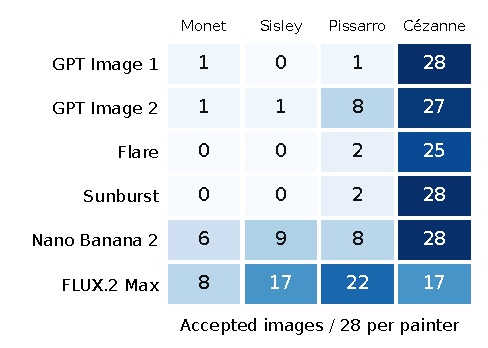
\includegraphics[width=\linewidth]{icml_selective_coverage.pdf}
\caption{Primary CSD gate: accepted images per prompted painter, out of 28
in every cell. Selection concentrates on C\'ezanne in several configurations;
the zero aggregate errors for GPT Image 1, Flare and Sunburst in
Table~\ref{tab:selective-main} coexist with missing painter conditions.
Counts describe prompt-name coverage, not painter fidelity.}
\label{fig:selective-coverage}
\end{figure}

The pre-outcome operational criterion required at least 50\% coverage in each
configuration, some accepted query from every painter, and positive mean error
reductions against both comparisons. The primary setting fails the first two
conditions. All eight encoder/view/target settings fail at least the coverage
condition; this 50\% requirement is a chosen operating point, not a universal
standard. CLIP's original-primary mean reductions are 12.1 and 1.7 points,
with minimum coverage 49.1\%. The complete continuous results and scene deletions
remain in Appendix~\ref{app:selective}.

The primary gate also assigns a name to 14.3--50.0\% of artist-free controls
and 17.9--75.0\% of generic-painting controls. These are assignments without a
requested name, not verified visual misattributions. The operational lesson
is to report per-painter coverage and a matched-coverage comparison before
using reduced accepted error as evidence for a useful attribution policy.
The test does not establish that abstention generally fails, and no replacement
rule is selected after these outcomes.

\section{Discussion}\label{sec:discussion}
Detecting a name response and matching painter differences are distinct achievements.
FLUX's lowest uncalibrated error in the 31-feature metric coexists with weak
Monet--Sisley alignment, while learned representations yield positive pair alignment.
Model comparisons should therefore report overall and pairwise scores together
for the stated reference target, distinguishing estimates from resolved comparisons.
Reports should also state whether they score each scene, the average pattern,
or rescaled contrasts. For prompted-name recognition, the two held-scene
controls distinguish sensitivity to a pooled domain offset from supervised
within-generator separability. The abstention test adds a second decision check: lower accepted error can
coexist with missing painters and little advantage over margin filtering.
Neither lower contrast error nor better name recovery alone establishes closer
painter resemblance.

The intervention identifies differences between prompt conditions, not their
internal causes. Training composition, guidance and shared transformations remain
possible explanations.

\subsection{Scope and Remaining Limitations}
The target is the pattern of differences in a finite digital reference
collection. It mixes subject choices and reproduction processes with properties
of the paintings. Coarse content classes do not match composition, viewpoint,
career period or actual generated scene adherence. The source audit addresses
visible peripheral regions and title/visual-class disagreements, but AI
judgments, uncertain boundaries and remaining capture differences limit that
correction. One reproduction per work cannot separate effects of illumination,
sharpening, conservation or digitization source.

The 31 coordinates describe digital color, spatial organization and texture;
neither they nor the learned encoders establish physical brushwork or perceived
painter resemblance. CSD's style-tag list includes all four painters, and exact
training-image overlap is unknown for both encoders. Numerical replay and
representation sensitivities do not validate perceptual judgments.
The main inference conditions on four related painters, 14 authored briefs,
two repeats and one clause template. The SD-Turbo check changes the template
and uses 25 matched-seed blocks, but retains the painter group and historical
target. Neither collection has a shared-family prompt control. A common response
could represent appropriate family-level style; its prevalence alone does not
establish a misleading or inferior response. Simulations probe stated noise
models, not actual service independence. The image panels
make the comparison inspectable, while incomplete public exact-pixel access
still limits independent measurement reproduction.

\section{Conclusion}
Shared change, labeled reference agreement and prompt-name recovery lead to
different evaluation conclusions. Common-majority naming change appears across
the complete metrics of two collections, but fails for SD-Turbo texture.
Monet--Sisley alignment depends on representation. Mean translation changes
name recovery without changing painter contrasts, while a reference-calibrated
abstention rule can lower accepted error by retaining a painter-skewed subset.
Reports should state the reference and aggregation target, partition proximity
gain, and accompany selective error with per-painter coverage and an
coverage-matched comparator. These measured cases support that evaluation
practice; they do not establish a general ranking of painter fidelity.


\section*{Reproducibility}
Versioned protocols, exact prompts, request configurations, source metadata,
scalers and retained feature vectors support numerical replay. The primary
analysis, post-result diagnostics and source-quality sensitivities have separate
input hashes and replay commands (Appendix~\ref{app:icml-reproducibility}). Independent
feature re-extraction requires exact pixels, which remain outside the compact
repository; public recoverability of the current full image cohort is incomplete.
Identifying repository links are omitted from this anonymous draft.
\label{sec:main-end}
\clearpage
\section*{Impact Statement}
This work studies how to interpret measured responses to artist-name prompts.
It may help evaluation practitioners avoid treating prompt responsiveness or
proximity to a digital collection as evidence of artistic fidelity. Conversely,
misreading the measurements as a quality ranking could misrepresent artists,
reproductions or service capabilities. Reference and development reproductions
carry recorded source-license metadata, including public-domain, CC0 and
CC BY/BY-SA records; complete attribution and release packaging remain
outstanding. No living-artist study or human-participant evaluation is reported.
The measurements do not establish legal authorization, attribution
or perceptual authenticity. AI assistance was used in manuscript editing and
in the explicitly described reference-image audit; that audit has not been
human validated.
\bibliographystyle{icml2026}
\bibliography{references,icml_references}
\clearpage
\appendix
\onecolumn
\section{Feature Definitions}\label{app:features}
\begin{table}[!htbp]
\caption{The 31 fixed digital features. Counts refer to scalar coordinates.
Texture measurements do not measure physical paint relief or authenticate brushwork.
Exact scales and definitions appear in Appendix~\ref{app:features}.}
\label{tab:features}

\centering\small
\begin{tabularx}{\linewidth}{@{}>{\raggedright\arraybackslash}p{.15\linewidth}>{\raggedright\arraybackslash}p{.35\linewidth}>{\raggedright\arraybackslash}X@{}}
\toprule
Family & Measurements & Interpretation\\
\midrule
Color (11) & Lightness and chroma median/IQR; chromatic fraction; hue
concentration and entropy; color differences at three lags and their slope &
Brightness, color strength and diversity, and how rapidly colors change over space.\\[4pt]
Spatial (8) & Spectral slope, residual and anisotropy; orientation entropy;
horizontal--vertical balance; gradient median/IQR; quadrant divergence &
Coarse versus fine organization, dominant directions, edge strength and regional
variation in orientation.\\[4pt]
Texture (12) & Four wavelet energies, slope and curvature; three local-binary-pattern
entropies; three local coefficients of variation &
Detail across scales, diversity of local patterns and local luminance contrast.\\
\bottomrule
\end{tabularx}


\end{table}

Color coordinates use CIELAB under D65 and the $2^\circ$ observer. Lightness
and chroma each contribute a median and IQR. Chromatic fraction is the share
of pixels with $C^*\geq5$. Hue concentration is the magnitude of the
chroma-weighted circular mean; hue entropy uses 24 equally spaced bins and is
normalized by their log count. Both use chroma weights and are zero when fewer
than 1\% of pixels are chromatic. At each of three lags (1\%, 4\% and 16\% of
the short side), the median is taken over pooled horizontal and vertical
CIEDE2000 differences. A log--log slope summarizes their
scale dependence \citep{sharma2005ciede}.

Spatial and texture coordinates use linear-sRGB luminance. A Tukey window
(parameter .1) precedes Fourier analysis. Thirty-two logarithmic radial bins
cover 4--128 cycles per short side; a Theil--Sen line gives spectral slope and
its root-mean-square residual. Power-weighted axial concentration measures
anisotropy. Scharr derivatives supply gradient median and IQR, an 18-bin
magnitude-weighted orientation entropy, and horizontal--vertical balance. Mean
Jensen--Shannon divergence of quadrant orientation histograms from the global
histogram measures regional variation.

Four log mean-squared detail energies come from a four-level undecimated
\texttt{db2} wavelet transform, followed by their linear slope and mean second
difference \citep{mallat1989wavelet}. Uniform local-binary-pattern entropy uses
$(P,R)=(8,1),(16,2),(32,4)$ on quantized luminance
\citep{ojala2002lbp}. Three median local coefficients of variation use window
widths obtained by rounding 1\%, 4\% and 16\% of the short side and increasing
even widths to the next odd integer, with a $10^{-6}$ mean floor.
The fixed implementation records boundary handling and stabilizing
constants. The separate scaler contains 101 Monet, 36 Sisley, 48 Pissarro and
36 C\'ezanne works. Equal painter mass is used to calculate each weighted
median and IQR.

\section{Estimator Details and Sensitivity Analyses}\label{app:estimation}
Let $\theta_{msa}=\mathbb E[d_{msak}]$ and
$d_{msak}=\theta_{msa}+\eta_{msak}$. If repeat errors have zero mean and
$\mathbb E\langle\eta_{msa1},\eta_{msa2}\rangle=0$, then
\[
 \mathbb E[\widehat D_{ms}]
 =H^{-1}\sum_a\|\theta_{msa}-r_a\|^2.
\]
Centering induces dependence between artists within a repeat, but independent
repeat blocks preserve the vanishing cross-repeat term. A common response has
$\theta_{msa}=0$ and hence expected $D=1$, even if it shifts the entire named
collection toward the references. A correctly aligned but rescaled response
$\theta_{msa}=b r_a$ gives expected $D=(b-1)^2$. Orthogonal deviations add their
squared magnitude. This identity explains why stronger painter contrasts need not have lower
reference-relative squared error.

The aggregate error $D_{\rm aggregate}$ applies the cross-product estimator to scene-averaged
contrasts; Equation~\ref{eq:scene-decomposition} relates it to the primary,
equally scene-weighted error. Painters also receive equal weight. Their
additive contributions sum to $D$, but centering couples the four conditions,
so these contributions are not standalone artist-fidelity scores.

For a model contrast, compute one error difference per complete paired scene.
Its standard error is the sample standard deviation of those differences divided
by $\sqrt n$. The simultaneous half-width is
$t_{n-1,1-.05/(2\cdot21)}\,\mathrm{SE}$. Six aligned-response intervals use the same
family adjustment. Additional nominal intervals and 5,000 paired-scene bootstrap
draws are descriptive checks, not alternative routes to significance. Reference
sensitivity draws 1,000 bootstrap samples independently within each painter,
recomputes reference means and $H$, and holds generated vectors and scaling
fixed. It describes reference-panel dependence rather than all uncertainty
jointly.

Declared before inspecting the new feature outcomes, the four-class reference
sensitivity uses a fixed lexicon applied to source titles: water-organized, built-place-organized, route-organized, and open or
wooded land. Each class mean receives one-quarter weight within a painter.
Resampling within artist/class strata conditions on those labels and does not
account for classification error. The older controlled naming panel used a
separate three-class visual coding scheme, described below.

For the shared-effect diagnostic, average each arm over scenes within repeat.
With named-minus-free differences $h_{ak}$ and $c_k=\frac14\sum_a h_{ak}$,
common and specific squared magnitudes are $4\langle c_1,c_2\rangle$ and
$\sum_a\langle h_{a1}-c_1,h_{a2}-c_2\rangle$. Their common fraction is reported
when the total is positive; corrected components may be negative. The within-scene
version computes both squared-change components separately in each scene,
averages each over scenes, then takes their ratio. Its shares range from 88.6\%
(GPT Image 1) to 97.2\% (FLUX).
Let $g_k$ be the generic-minus-free shift. The ordinary repeat-averaged cosine
shares a noisy free estimate in both vectors, adding its error covariance trace
to the expected numerator. The corrected cosine reported in
Section~\ref{sec:shared-change} instead uses cross-repeat products,
$[\langle g_1,c_2\rangle+\langle g_2,c_1\rangle]/
[2\sqrt{\langle g_1,g_2\rangle\langle c_1,c_2\rangle}]$ when both norm squares
are positive. The ratio itself is not unbiased or constrained to $[-1,1]$.
Primary $D$ uses only named arms and is unaffected by shared-free-control noise.

\subsection{Additional Score Identities}\label{app:score-details}
Under a shared affine transformation $z\mapsto Az+b$, centering removes
the additive term $b$ but leaves the transformed contrast $Ad$.

The estimator has an exact decomposition. Write
$e_{msak}=d_{msak}-\widehat\beta_{msk}r_a$. Then
\begin{equation}
 \widehat D_{ms}=
 (\widehat\beta_{ms1}-1)(\widehat\beta_{ms2}-1)
 +\frac1H\sum_a\langle e_{msa1},e_{msa2}\rangle.
 \label{eq:decomposition}
\end{equation}
The first term measures reference-aligned amplitude error. The residual is
orthogonal to the single stacked reference configuration; it is not necessarily
outside the feature-space span of the reference means, much less outside all
authentic artistic variation. Both terms can be negative in finite samples.

Let $\theta_s$ stack the four conditional mean contrasts and
$\bar\theta=S^{-1}\sum_s\theta_s$. The population target decomposes as
\begin{equation}
 D_{\rm scene}=\frac{\|\bar\theta-r\|^2}{H}
 +\frac1{SH}\sum_s\|\theta_s-\bar\theta\|^2
 =D_{\rm aggregate}+V_{\rm scene}.
 \label{eq:scene-decomposition}
\end{equation}
To separate contrast strength from direction, define
\begin{equation}
 \widehat Q_m=\frac1{SH}\sum_{s,a}\langle d_{msa1},d_{msa2}\rangle,
 \qquad \widehat D_m=1-2\widehat\beta_m+\widehat Q_m.
 \label{eq:magnitude}
\end{equation}
For positive $\widehat Q_m$, $\widehat\beta_m/\sqrt{\widehat Q_m}$ is a
noise-corrected alignment summary; finite estimates need not lie in $[-1,1]$.
Scaling every centered generated contrast by $c$ gives
$\widehat D_m(c)=1-2c\widehat\beta_m+c^2\widehat Q_m$.
We fit $c=\max(0,\widehat\beta/\widehat Q)$ on the other 13 scenes and evaluate
it on the held-out scene. The fitting criterion is available only when its
training $\widehat Q$ is positive, as it is in every observed fold. This
counterfactual concerns feature vectors, not an implemented image transformation.

\subsection{Paired Comparisons and Declared Sensitivities}\label{app:declared-sensitivities}
We fit the scene fixed-effects regression
\begin{equation}
 \widehat D_{ms}=\alpha_s+\gamma_m+\varepsilon_{ms},
 \qquad\gamma_{\text{GPT Image 2}}=0.
 \label{eq:regression}
\end{equation}
In the balanced panel, coefficient differences equal the paired scene means
used for inference. Changing the regression baseline leaves these differences
unchanged; Table~\ref{tab:specificity-models} presents them relative to FLUX.
Declared sensitivities delete each scene, resample scenes
and reference works, examine feature families and omit texture. Central-square
windows control aspect ratio by discarding peripheral content in generated and
reference images. FLUX retains the lowest uncalibrated error after every scene
deletion ($D=.754$--$.852$) and with square windows ($D=.765$; next-lowest
Nano Banana 2, $1.024$).

\subsection{Distributional Proximity and Repeat Spread}
For painter $a$, energy discrepancy compares its generated collection $Y_a$
with reference collection $X_a$:
\begin{equation}
 \E(X,Y)=\frac{2}{n_Xn_Y}\sum_{i,j}\|x_i-y_j\|
 -\frac1{n_X^2}\sum_{i,i'}\|x_i-x_{i'}\|
 -\frac1{n_Y^2}\sum_{j,j'}\|y_j-y_{j'}\|.
 \label{eq:energy}
\end{equation}
Its finite-sample expectation depends on within-collection spread; equal
generated sample sizes do not eliminate comparison bias. Appendix~\ref{app:diagnostics}
gives the correction for the repeated-scene design. Within-scene repeat spread,
$\frac{1}{2S}\sum_s\|z_{msa1}-z_{msa2}\|^2$, is the mean sample-variance
trace of the two outputs. It separates repeat dispersion from variation across
briefs.


\section{Post-result Target Diagnostics}\label{app:diagnostics}
These retrospective analyses retain the completed 1,008 generated images and
the original inferential family. The initial diagnostics use unchanged reference
vectors and scaling; the subsequent source audit separately varies painting
regions, development scaling and content labels.

\subsection{Content-specific Targets and Genuine-painting Controls}
The recorded reference classes are water-organized, built-place-organized,
route-organized, and open or wooded land, assigned by a fixed source-title
lexicon. Counts in that order are $(191,67,8,31)$ for Monet, $(52,29,9,16)$ for
Sisley, $(28,77,12,24)$ for Pissarro and $(31,28,12,34)$ for C\'ezanne.
Class-specific means are centered across painters just as in the pooled target.
Their mean squared departure from the pooled target is $.438H$, a description
of observed reference means that includes finite-sample error.

For the generated comparison, the four water, four built and three land briefs
use the corresponding class means; the three mixed briefs are excluded.
We average the class-specific cross-product error over these $S=11$ scenes and divide by
$H_c=S^{-1}\sum_s\sum_a\|r_{a,c(s)}\|^2=7.413$, compared with pooled $H=5.915$.
Each column of Table~\ref{tab:review-targets} therefore has its own denominator.
The unchanged 11-scene pooled comparison isolates the scene-subset choice.
These title-derived strata have 16--191 reference works per artist/class among
the three included classes, but do not supply visually matched historical scenes.

For each of 1,000 genuine-painting controls, works in each artist/class cell
are randomly divided into disjoint halves, with the smaller half used for
target estimation. A pooled control samples two independent works with replacement
from each painter's held-out half for each of 14 pseudo-scenes. A class-stratified
control samples within the held-out class for each of the 11 water, built or
land pseudo-scenes. It is compared with both pooled and class-specific means
from the training halves, using each target's own squared magnitude.
The random seed is 2026091201. Sampling can repeat a held-out work, but no
held-out work is used to estimate that split's target. The development scaler
is fixed throughout.

To separate sparse sampling from changes in the comparison pools, we also
calculate each split's expected score from its exact held-out means, keeping
the training target and normalizer fixed (Table~\ref{tab:painting-control-ranges}).

\begin{table}[htbp]
\caption{Central 95\% ranges of genuine-painting control scores across 1,000
splits. Exact means integrate out sampling within each split; these finite-pool
ranges are not confidence intervals.}
\label{tab:painting-control-ranges}

\centering\small
\begin{tabular}{llcc}
\toprule
Control sampling & Reference target & Two draws & Exact held-out means\\
\midrule
Pooled & Pooled & $[-.758,1.380]$ & $[.135,.428]$\\
Class-stratified & Pooled & $[-.554,2.400]$ & $[.544,.993]$\\
Class-stratified & Class-specific & $[-.248,1.946]$ & $[.517,.954]$\\
\bottomrule
\end{tabular}


\end{table}

For pooled controls, SD falls from $.561$ to $.076$ after integrating out
sampling. These controls still condition on imperfect title classes and a
single source capture per work; they do not calibrate artistic fidelity.

\begin{table}[htbp]
\caption{Descriptive error under alternative targets and metrics. The class target uses title-derived water, built and land strata; the three mixed briefs are excluded. Each column uses its own reference normalizer; absolute values across columns are not directly comparable. Covariance is fitted only on development works, with fixed 50\% shrinkage.}
\label{tab:review-targets}
\centering\small
\begin{tabular}{@{}lrrrr@{}}\toprule
 & \multicolumn{2}{c}{11 common briefs} & \multicolumn{2}{c}{14 briefs}\\
Model & Pooled target & Class target & Equal family & Covariance\\\midrule
GPT Image 1 & 1.557 & 1.366 & 1.551 & 2.103\\
GPT Image 2 & 1.099 & 1.130 & 1.243 & 1.511\\
2.5 Flare & 1.726 & 1.539 & 1.765 & 1.636\\
2.5 Sunburst & 1.633 & 1.525 & 1.680 & 1.617\\
Nano Banana 2 & 0.987 & 0.948 & 1.203 & 1.385\\
FLUX.2 Max & 0.750 & 0.786 & 0.808 & 0.928\\
\bottomrule\end{tabular}

\end{table}

\FloatBarrier

\subsection{Magnitude, Artist Coverage and Coordinate Weighting}\label{app:magnitude-coverage}
The cross-repeat version of Equation~\ref{eq:scene-decomposition} is exact for
the retained vectors. Its variation term replaces squared deviations with
cross-products between scene-centered repeats. The term can be negative in
finite samples, although its independent-repeat population target is nonnegative.
Scalar calibration fits only the other 13 scenes. All fold denominators $Q$
are positive. GPT Image 2's fitted scalars range from .438 to .459 and FLUX's
from .598 to .694; all fold-specific scores are retained. No calibration
parameter is selected by minimizing its own held-out score. The subsequent
deletion check refits the entire procedure on
each remaining 13-scene panel, rather than treating overlapping folds as
independent replications. Its mean GPT Image 2-minus-FLUX error differences
range from $-.189$ to $-.137$.

\begin{table}[htbp]
\caption{Descriptive magnitude and alignment of painter contrasts. $Q=1$ equals the reference squared size, and $D=1-2\beta+Q$. The alignment ratio can fall outside $[-1,1]$ in finite samples.}
\label{tab:review-alignment}
\centering\small
\begin{tabular}{@{}lrr@{}}\toprule
Model & Squared contrast magnitude $Q$ & Alignment ratio $\beta/\sqrt Q$\\
\midrule
GPT Image 1 & 2.449 & 0.600\\
GPT Image 2 & 2.223 & 0.670\\
2.5 Flare & 2.281 & 0.511\\
2.5 Sunburst & 2.289 & 0.545\\
Nano Banana 2 & 0.994 & 0.444\\
FLUX.2 Max & 0.741 & 0.546\\
\bottomrule\end{tabular}

\end{table}


For artist pairs, both generated and reference contrasts are direct differences
between the two artists; the denominator is the squared reference-pair distance.
Leaving one artist out recenters the remaining three generated and reference
conditions. Reference singular components are the three rank-one terms of the
centered four-by-31 reference matrix: each combines an artist contrast with a
feature direction, rather than representing one artist. Component aligned
responses project onto each term separately.

\begin{table}[htbp]
\caption{Descriptive artist coverage of the aligned response. Reference components account for 66.3\%, 20.6\% and 13.0\% of centroid variation. Each omission recomputes the target and recenters the other three artists.}
\label{tab:review-components}
\centering\small
\begin{tabular}{@{}lrrr|rrrr@{}}\toprule
 & \multicolumn{3}{c}{Component aligned response} & \multicolumn{4}{c}{Aligned response after omitting}\\
Model & First & Second & Third & Monet & Sisley & Pissarro & C\'ezanne\\\midrule
GPT Image 1 & 1.248 & 0.310 & 0.356 & 1.140 & 1.072 & 0.840 & 0.389\\
GPT Image 2 & 1.156 & 0.617 & 0.800 & 1.195 & 0.972 & 0.992 & 0.651\\
2.5 Flare & 1.022 & 0.211 & 0.383 & 1.034 & 0.734 & 0.802 & 0.222\\
2.5 Sunburst & 1.082 & 0.250 & 0.417 & 1.116 & 0.840 & 0.762 & 0.284\\
Nano Banana 2 & 0.513 & 0.371 & 0.195 & 0.569 & 0.446 & 0.388 & 0.276\\
FLUX.2 Max & 0.666 & 0.021 & 0.183 & 0.539 & 0.511 & 0.527 & 0.096\\
\bottomrule\end{tabular}

\end{table}


Table~\ref{tab:review-components} shows that aggregate positive alignment is
uneven across those components.

Equal-family weighting assigns each coordinate inverse family size (11, 8 or 12).
The covariance sensitivity uses 221 development works with equal painter mass.
For their weighted covariance $\Sigma$, the metric is
$[.5\Sigma+.5\operatorname{tr}(\Sigma)I/31]^{-1}$, with fixed shrinkage and no
tuning on evaluated images. These weighting choices are not independently
validated artistic metrics.

\begin{samepage}
FLUX retains the lowest point estimate under all
31 single-coordinate deletions; the report retains every coordinate contribution,
including negative terms.
Without texture, Flare and Sunburst still have error estimates above the
no-contrast value of one (1.580 and 1.604).
\end{samepage}

\subsection{A Design-aware Energy Correction}
The primary energy values use empirical distributions, including their zero
diagonal distances. To estimate energy between a fixed empirical reference
and the equally weighted mixture of scene-conditional output distributions,
cross-scene generated pairs already have the required independent draws.
Only the same-scene generated term needs adjustment. With two repeats and
$S$ scenes, the descriptive correction is
\[
 \widehat{\mathcal E}_{\rm strata}
 =\widehat{\mathcal E}_{\rm empirical}
 -\frac{1}{2S^2}\sum_s\|y_{s1}-y_{s2}\|.
\]
The reference within-distance remains empirical because this target conditions
on the finite reference panel. A pooled IID $n/(n-1)$ multiplier would also
alter cross-scene terms and estimate a different target. This correction retains
the 21 negative named-minus-generic differences. It does not solve unequal
historical and generated content mixtures, and no new energy tests are performed.

\subsection{Uncertainty and Synthetic Coverage Checks}
The Student procedure uses 14 scene summaries. For independent scene errors
with fixed conditional means $\delta_s$, its estimated variance has expectation
\[
 \mathbb E[s_\delta^2/S]
 =\operatorname{Var}(\bar{\widehat\delta})
 +\frac{1}{S(S-1)}\sum_s(\delta_s-\bar\delta)^2.
\]
It therefore includes real between-scene heterogeneity as well as request noise.
This explains why it is not a direct estimate of fresh-request variance for
exactly the fixed panel. It also does not provide an exact coverage guarantee:
non-Gaussian cross-products and dependence can affect the Student approximation.

The initial 5,000-run scenarios (seed 2026091202) use the six configurations,
14 scenes, two repeats and 21-endpoint family, with unit reference magnitude.
Gaussian, variance-standardized $t_3$/heteroskedastic and fixed scene-interaction
errors give simultaneous coverage 95.96\%, 97.42\% and 99.68\%. Their independent
centered noise power is $.5$. Allocating half the noise to a model-specific
state shared by all scenes and both repeats reduces coverage to 0.04\%, with
mean corrected-error bias near $.25$.

A subsequent sweep uses independent Gaussian errors at powers $.5$, $1.5$ and
$3$, with either isotropic or rank-three covariance aligned with the reference
components (5,000 runs per case). Coverage ranges from 95.06\% to 96.80\%, with
Monte Carlo SE $.25$--$.31$ percentage points. For comparison, directly centered
repeat differences estimate observed powers of $.424$--$2.596$ relative to $H$.
These stress models probe coverage approximations, not actual service independence;
no significance threshold is selected from them.

\subsection{Source-quality Sensitivity}\label{app:reference-quality}
AI assistants inspect all 649 reference and 221 development reproductions
using contact sheets and enlarged peripheral regions, recording removable
calibration targets, frames, margins and labels. Uncertain boundaries remain
unchanged. Reference content is visually classified before comparison with the
title label; mixed or unclear cases retain that label.

The audit selects crops for 90 reference and 41 development images, including
ten calibration-strip cases; 43 uncertain boundaries remain unchanged. Visual
classes differ from 230 title assignments, while 42 mixed or unclear cases
retain their original labels. These AI-coded sensitivities did not undergo human verification and are not
independent ground truth.

Audited rectangular crops follow the original orientation and ICC rules, before
aspect-preserving Lanczos resizing to a 512-pixel short side without upsampling.
All 31 features and all works are retained. We compare corrected references with
original scaling, then refit development IQR scaling and consistently transform
generated vectors. Label sensitivity uses the same 11 briefs. Versioned records
preserve audit decisions, new vectors and original results; model scores do not
select corrections.
All six aligned-response intervals remain above zero with either scaler.
With original scaling, corrected regions give FLUX $D=0.832$.
After refitting, (uncalibrated, held-out calibrated) errors are:
GPT Image 1 $(1.631,0.693)$, GPT Image 2 $(1.259,0.579)$,
Flare $(1.737,0.760)$, Sunburst $(1.577,0.711)$, Nano Banana 2 $(1.121,0.846)$
and FLUX $(0.872,0.762)$. FLUX and GPT Image 2 retain the respective minima.

\section{Image Selection and Provenance}\label{app:images}

\begin{figure}[p]
\centering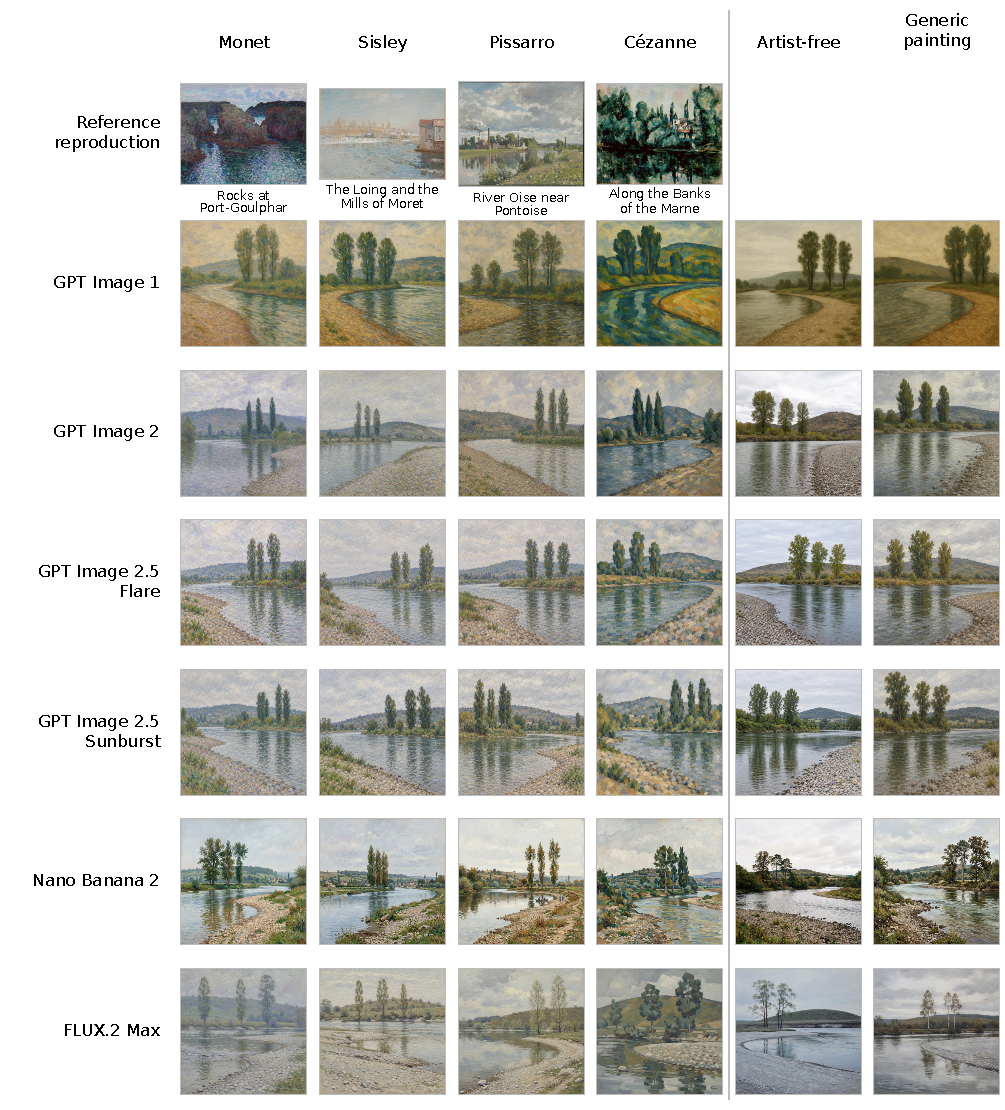
\includegraphics[width=\linewidth]{specificity_original_generated.pdf}
\caption{One scene, six prompt conditions and six generators. The requested scene
is a broad river bending past a gravel bank, three trees on the opposite bank,
and a low hill under an overcast sky. In each model row, compare the four named
outputs with the artist-free and generic oil-painting controls on the right,
then compare the painter names with one another. The top row shows audited
reference regions for display; primary scores use full frames. These works were
neither generator inputs nor matched compositions. All generated examples use the first brief and first
repeat; Appendix~\ref{app:images} gives the full prompt, selection rule and provenance.}
\label{fig:original-generated}
\end{figure}

The generated examples use the first declared brief and first repeat, selected
after analysis without appearance- or score-based curation. The brief reads:
``A broad river bends past a gravel bank. Three tall trees stand on the far bank,
with a low hill behind them under a pale overcast sky.'' Every prompt ends with
``No text or frame.'' Only the clauses in Section~\ref{sec:design} change.

References in Figure~\ref{fig:original-generated} are the lexicographically first
measured work IDs per painter classified as water-organized in the completed
audit, with recorded public-domain status. The Sisley and Pissarro reproductions
use audited crops removing calibration strips; Monet and C\'ezanne retain their
full regions. The manifest records image identities, provenance, crop boxes
and exact prompts. The paintings are not matched to the generated brief.


\FloatBarrier


\section{Complete Model and Painter Summaries}\label{app:results}
Tables~\ref{tab:all-specificity-pairs}--\ref{tab:artist-distributions} and
Figures~\ref{fig:specificity-diagnostics}--\ref{fig:specificity-distributions}
summarize model comparisons, error components and collection-level proximity
and spread.
\emph{Energy discrepancy} combines between-collection distances and internal
spread; lower values mean greater proximity (Appendices~\ref{app:estimation}
and~\ref{app:diagnostics}). Naming lowers energy relative to the generic clause in 21 of 24
model--painter cells, including the correction for repeated scenes.
All 24 named collections have smaller total feature variance than their historical
counterparts. These descriptive comparisons use 28 named or generic outputs
against the recorded reference panel, with different subject mixtures; they do
not establish agreement of painter contrasts.
\begin{table}[htbp]
\caption{All 15 paired model comparisons in the prespecified inferential family. Intervals are approximate 95\% simultaneous intervals adjusted across all 21 endpoints. A negative contrast favors model A on the stated feature-geometry target.}
\label{tab:all-specificity-pairs}
\centering\small
\begin{tabular}{llr}\toprule
Model A & Model B & $D_A-D_B$ [simultaneous interval]\\\midrule
GPT Image 1 & GPT Image 2 & $0.346\;[-0.400,1.093]$\\
GPT Image 1 & 2.5 Flare & $-0.165\;[-1.027,0.697]$\\
GPT Image 1 & 2.5 Sunburst & $-0.069\;[-1.181,1.043]$\\
GPT Image 1 & Nano Banana 2 & $0.463\;[-0.602,1.528]$\\
GPT Image 1 & FLUX.2 Max & $0.771\;[-0.037,1.580]$\\
GPT Image 2 & 2.5 Flare & $-0.512\;[-1.150,0.126]$\\
GPT Image 2 & 2.5 Sunburst & $-0.415\;[-1.181,0.350]$\\
GPT Image 2 & Nano Banana 2 & $0.116\;[-0.922,1.155]$\\
GPT Image 2 & FLUX.2 Max & $0.425\;[-0.161,1.011]$\\
2.5 Flare & 2.5 Sunburst & $0.096\;[-0.286,0.478]$\\
2.5 Flare & Nano Banana 2 & $0.628\;[-0.283,1.540]$\\
2.5 Flare & FLUX.2 Max & $0.937\;[0.256,1.618]$\\
2.5 Sunburst & Nano Banana 2 & $0.532\;[-0.436,1.500]$\\
2.5 Sunburst & FLUX.2 Max & $0.840\;[0.058,1.623]$\\
Nano Banana 2 & FLUX.2 Max & $0.309\;[-0.847,1.464]$\\
\bottomrule\end{tabular}

\end{table}

\begin{table}[htbp]
\caption{Complementary empirical distribution summaries. Energy change is named-minus-generic reference energy; variance ratios are generated-to-reference. Negative changes favor naming; ratios below one indicate narrower generated feature distributions.}
\label{tab:artist-distributions}
\centering\small
\begin{tabular}{llrrrr}\toprule
Model & Measure & Monet & Sisley & Pissarro & C\'ezanne\\\midrule
GPT Image 1 & Energy change & $-2.515$ & $-2.739$ & $-2.628$ & $-1.336$\\
& Variance ratio & $0.479$ & $0.694$ & $0.603$ & $0.598$\\
\addlinespace[2pt]
GPT Image 2 & Energy change & $-0.602$ & $-1.092$ & $-0.195$ & $-0.373$\\
& Variance ratio & $0.283$ & $0.312$ & $0.303$ & $0.303$\\
\addlinespace[2pt]
2.5 Flare & Energy change & $0.962$ & $-0.008$ & $0.429$ & $-1.013$\\
& Variance ratio & $0.269$ & $0.371$ & $0.321$ & $0.275$\\
\addlinespace[2pt]
2.5 Sunburst & Energy change & $0.267$ & $-0.718$ & $-0.091$ & $-1.653$\\
& Variance ratio & $0.248$ & $0.274$ & $0.273$ & $0.318$\\
\addlinespace[2pt]
Nano Banana 2 & Energy change & $-0.513$ & $-1.381$ & $-0.741$ & $-1.102$\\
& Variance ratio & $0.829$ & $0.708$ & $0.572$ & $0.877$\\
\addlinespace[2pt]
FLUX.2 Max & Energy change & $-0.707$ & $-0.886$ & $-1.080$ & $-1.431$\\
& Variance ratio & $0.340$ & $0.416$ & $0.570$ & $0.622$\\
\bottomrule\end{tabular}

\end{table}

\FloatBarrier

\begin{figure}[tbp]
\centering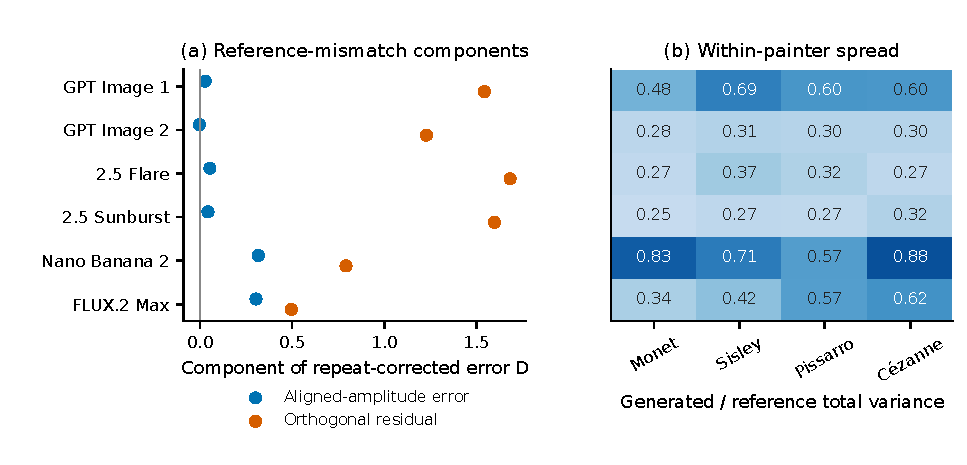
\includegraphics[width=\linewidth]{specificity_diagnostics.pdf}
\caption{Descriptive summaries for the original reference target.
(a) Amplitude error and the orthogonal residual---differences perpendicular to
the overall labeled reference pattern---sum to $D$ (Equation~\ref{eq:decomposition}).
(b) Generated/reference variance ratios for every model and painter. Total
spread includes variation across fixed briefs and is not a mode-collapse measure.}
\label{fig:specificity-diagnostics}
\end{figure}
\begin{figure}[tbp]
\centering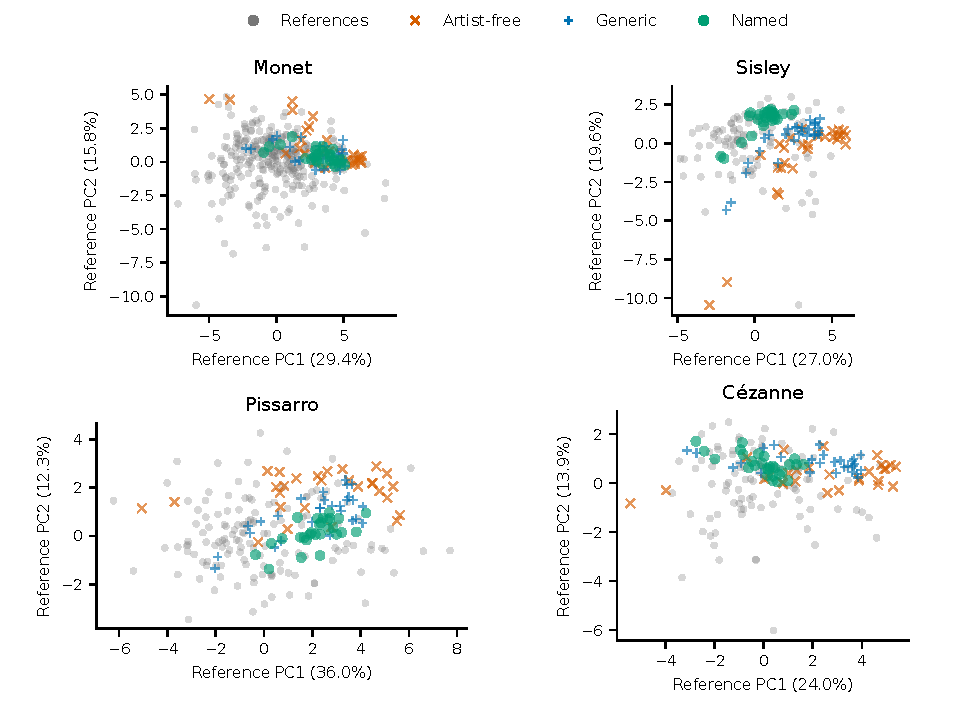
\includegraphics[width=.92\linewidth]{specificity_sunburst_distributions.pdf}
\caption{GPT Image 2.5 Sunburst's named outputs appear more concentrated than
the reference works in all four projections. This model illustration was selected before the
primary feature outcomes were inspected. Each panel uses principal components
fitted only to that painter's reference works, so axes differ between painters.
The 14 generated briefs and two repeats have a different content distribution
from the historical panel. Projections are descriptive; numerical summaries
use all 31 coordinates.}
\label{fig:specificity-distributions}
\end{figure}
\FloatBarrier

\section{Supporting Interventions}\label{sec:why}\label{app:cohorts}
These earlier cohorts address related but different questions
(Table~\ref{tab:cohorts}). They are not pooled with the six-model experiment
or treated as independent-investigator replications. Historical model labels
identify recorded request configurations, not verified underlying models
(Appendix~\ref{app:provenance}).

\begin{table}[htbp]
\caption{Supporting evidence is kept separate from the new six-model experiment.
Different prompts, panels and finite-sample targets do not form one pooled test.}
\label{tab:cohorts}

\centering\small
\begin{tabularx}{\linewidth}{@{}>{\raggedright\arraybackslash}p{.22\linewidth}>{\raggedright\arraybackslash}p{.27\linewidth}>{\raggedright\arraybackslash}X@{}}
\toprule
Cohort & Comparison & Role in this paper\\
\midrule
Four-painter exploration & 649 references; 1,920 generated outputs &
Describes reference/generated separation and motivates the controlled test.\\[4pt]
Controlled naming & 1,006 outputs; 38 Monet and 32 C\'ezanne references &
Six named/free and two detailed/short prompt contrasts; subsequent transformation
and conditional-variance diagnostics.\\[4pt]
Palette interventions & Two separate 192-output collections &
Named-minus-generic chroma response; no pooling across collections.\\[4pt]
Generic-clause comparison & 96 C\'ezanne/generic outputs on 24 new scenes &
Tests a proximity gain beyond a generic painting clause.\\[4pt]
Fixed-map transfer & 240 FLUX/C\'ezanne outputs on 12 new scenes &
Prospective counterexample to the historical opposing energy/prediction ordering.\\
\bottomrule
\end{tabularx}


\end{table}

\subsection{Proximity and Spread under Naming}
The four-painter exploration used 1,536 named and 384 artist-free outputs,
three prompt methods and 16 scenes. Its 24 model--painter--method cells had
total variance ratios .206--.376 and grouped generated/reference discrimination accuracy
.940--.983. Pooled named energy medians for Monet, Sisley, Pissarro and C\'ezanne
were 2.068, 1.678, 1.975 and 2.142; corresponding artist-free medians were
1.732, 1.878, 1.854 and 1.657. Only Sisley had a lower pooled named median.
Matched-size real/real medians were .193, .215, .164 and .199. These post-result
summaries describe that exploration, not a general naming effect.

The later controlled panel selected Monet and C\'ezanne after exploration.
It crossed 24 scenes with three models, two clauses and three repeats; 142
short-scene outputs supplied two prompt-length comparisons. Reference panels
contained 38 Monet and 32 C\'ezanne works, with water/built/land masses based on
maintainer-run LLM visual coding. Named-minus-free energy changes were
$-.846,-1.818$ for Nano Banana 2, $-.625,-.896$ for FLUX, and $-.234,-.056$ for
GPT Image 2 (Monet, C\'ezanne). The first four null hypotheses were rejected in
the original family of eight. A separate 72-output FLUX collection repeated both directions
($-.695,-.952$) with rejection in its own four-endpoint family.

A standalone 96-output GPT Image 2/C\'ezanne comparison on 24 new scenes reduced energy
relative to the generic clause by 1.195 ($p=.00001$, fixed $\alpha=.025$), with
named/generic total variance ratio .552. It randomized clauses within 48 two-position
blocks, used reference class masses $(3,11,18)/32$, and tested a sharp no-effect
null with 99,999 within-block sign draws and plus-one correction. This tests
clause effects, not equality of energy alone. A generic clause therefore did
not reproduce the full proximity gain in that panel, but proximity does not
establish correct four-artist contrasts. Likewise, lower total spread does
not establish loss of scene information: controlled FLUX/Monet held-repetition
scene retrieval rose from 44.4\% to 59.7\% under naming. This measures relative
feature distinguishability, not verified prompt adherence.

\subsection{Palette Responsiveness and a Contrary Transfer Result}
Both 192-output palette collections requested the historical GPT Image 2 alias,
using six scenes, four repeats, muted/vivid instructions and free, generic,
Monet and C\'ezanne clauses. Primary name-minus-generic chroma-response
interactions were unresolved (Monet, C\'ezanne):
$-.284,-.018$ in the first collection and $-.159,.037$ in the later one.
Their adjusted intervals spanned zero in the original two-interaction family and the later four-endpoint
family, which also included two FLUX naming contrasts.
Secondary generic-minus-free responses were $-.853$ and $-.891$, with nominal
95\% intervals excluding zero. Thus generic painting can attenuate measured
palette response without an identified additional name effect. Two palette
levels do not distinguish reduced gain from saturation or an operating-range
shift, and unresolved interactions do not demonstrate equivalence.

Earlier maps translated and optionally isotropically rescaled artist-free feature
vectors to predict named-prompt scene means, with fits based only on generated
images and evaluation on held-out scenes. Actual naming had lower reference energy than
translation plus isotropic scaling in all six model--painter averages. Adding
scale improved named-mean prediction in all six while worsening reference
energy in five. That ordering did not transfer to a prospective 240-output
FLUX/C\'ezanne comparison with 12 new scenes and ten repeats, using the original
fits unchanged. Translation/scaling improved both energy and repeat-corrected
prediction error relative to translation: $-.390\;[-.509,-.271]$ and
$-5.047\;[-7.880,-2.214]$, with approximate simultaneous jackknife intervals.
The achieved prediction-error half-width exceeded its planning criterion.
This contrary result is retained without extra sampling; it rules out treating
the historical opposing ordering as a universal mechanism. These named/free maps
differ from the retrospective calibration of painter contrasts in
Table~\ref{tab:review-calibration}.

\section{Collection Provenance and Computational Scope}\label{app:provenance}
Historical GPT Image 1 and GPT Image 2 labels identify the requested model
names. A later technical negative control showed that the earlier image
interface also accepted an invented image-model identifier. This does not show
that valid names select the same underlying model, but successful request
acceptance alone cannot authenticate their separation. Historical contrasts
are therefore interpreted as recorded request-group comparisons. The current
experiment uses explicit documented model identifiers and fixed routes;
it does not reuse historical images as verified examples of the new variants.
All current outputs decode to the requested square dimensions, but their
response bodies do not echo model or quality fields. Labels therefore denote
the documented request configurations, without independent checkpoint
attestation. Underlying checkpoints and training corpora are not available
for inspection.

The present experiment excludes technical probes and an earlier attempt closed
before feature measurement because model selection could not be qualified.
No image is shared between these collections. The earlier incomplete
generic-clause cohort is likewise not pooled with its complete 96-image
successor. Exact assignments, attempt outcomes and measurement exclusions are
retained in the versioned manifests; selection was not based on visual success.

\clearpage
\section{Projection of Labeled Painter Contrasts}\label{app:geometry}
In Figure~\ref{fig:specificity-geometry}, C\'ezanne remains visibly separated,
while generated Monet and Sisley means often lie close together. The M/S/P detail
boxes magnify the nearby positions. The axes combine the 31 standardized features, with directions fitted
only to the four reference means. Together they show 86.99\% of variation among
those means; Figure~\ref{fig:artist-pairs} checks all 31 features.

\begin{figure}[tbp]
\centering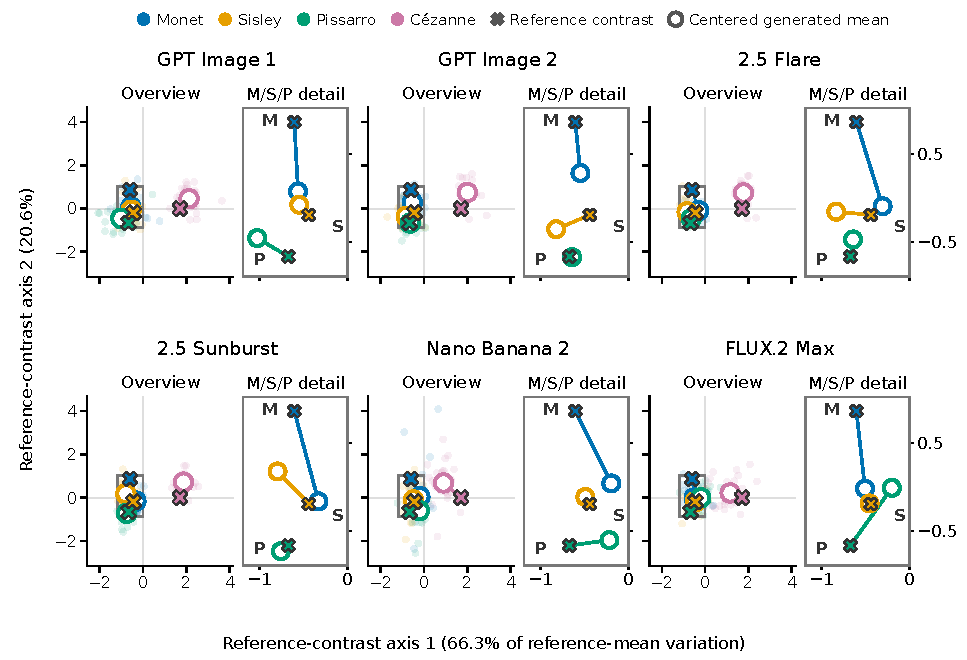
\includegraphics[width=\linewidth]{specificity_geometry.pdf}
\caption{Matching the labeled painter pattern. Crosses mark reference contrasts;
open circles average generated contrasts over all 14 scenes and both repeats.
Shorter matching-label lines indicate less projected mismatch;
faint dots show centered scene/repeat contrasts.
The outlined region is enlarged in the adjacent Monet (M), Sisley (S) and
Pissarro (P) detail at a common scale; C\'ezanne
remains in the overview. Each view uses common axes across models. Agreement
in these two projected axes does not establish agreement in all 31 features.}
\label{fig:specificity-geometry}
\end{figure}

\section{Direct Naming and Scene Influence}\label{app:direct-naming}
These analyses use the retained vectors and are retrospective. The full-frame
named-minus-generic shared fractions had already been inspected before the
version-three analysis plan was written; it is not a preregistration.
No new significance tests, images, coordinate choices or reference corrections
are introduced. The versioned report binds the plan, implementation, analytical
tests and retained inputs by SHA-256 and supports exact numerical replay.

\subsection{Changing the Baseline and Keeping the Cross Term}
For each model, average arm vectors over scenes within repeat $k$. Write $g_k$
for generic-minus-free, $n_k$ for mean-named-minus-generic and $c_k$ for
mean-named-minus-free. The vector identity $c_k=g_k+n_k$ implies
\begin{equation}
 \underbrace{4\langle c_1,c_2\rangle}_{C}
 =\underbrace{4\langle g_1,g_2\rangle}_{G}
 +\underbrace{4\langle n_1,n_2\rangle}_{N}
 +\underbrace{4\bigl(\langle g_1,n_2\rangle+
                    \langle n_1,g_2\rangle\bigr)}_{I}.
 \label{eq:generic-naming-identity}
\end{equation}
The between-name component $B=\sum_a\langle d_{a1},d_{a2}\rangle$ uses
scene-averaged, artist-centered vectors and is unchanged by switching the
baseline. Thus the free-baseline shared fraction is $C/(C+B)$, while the
generic-baseline fraction is $N/(N+B)$. Fractions are reported only for positive
totals; signed components are retained without clipping. The ratios are not
unbiased or necessarily bounded by zero and one. Table~\ref{tab:direct-naming-terms}
shows why $G+N$ alone does not recover $C$. The interaction $I$ is an algebraic
cross term, not a separately identified causal or internal model mechanism.

\begin{table}[htbp]
\caption{Retrospective full-frame decomposition in squared standardized feature units.
All terms use scene averages and cross-repeat products. $C=G+N+I$ exactly before rounding.}
\label{tab:direct-naming-terms}
\centering\small
\begin{tabular}{@{}lrrrrr@{}}\toprule
Configuration & Generic $G$ & Additional naming $N$ & Interaction $I$ & Common $C$ & Between-name $B$\\\midrule
GPT Image 1 & 29.812 & 31.122 & $-1.727$ & 59.207 & 12.518\\
GPT Image 2 & 37.175 & 29.450 & 6.242 & 72.867 & 12.074\\
2.5 Flare & 23.714 & 29.511 & 13.551 & 66.775 & 11.986\\
2.5 Sunburst & 18.194 & 23.485 & 19.373 & 61.052 & 11.738\\
Nano Banana 2 & 7.191 & 8.037 & 11.323 & 26.551 & 3.589\\
FLUX.2 Max & 22.371 & 31.590 & 38.619 & 92.580 & 4.149\\
\bottomrule\end{tabular}
\end{table}

\subsection{Scene Deletion and Measurement Windows}
Each deletion removes one scene, recomputes arm means over the remaining 13,
and then forms the cross-products and ratios. Table~\ref{tab:direct-naming-deletions}
retains the extrema over all deletions, with references and scaling fixed.
These ranges describe scene influence; they are not confidence intervals and
do not incorporate reference uncertainty or establish equivalence to zero.

For Monet--Sisley, let $q=\mu_{\rm Monet}-\mu_{\rm Sisley}$. The pair aligned
response is the average of
$\langle z_{ms,\rm Monet,k}-z_{ms,\rm Sisley,k},q\rangle/\|q\|^2$ over retained
scenes and repeats. Full-frame point estimates are $.074,.402,-.011,-.249,-.044,.129$
in table order; square-reference estimates are $.038,.408,.012,-.185,-.017,.132$.
Deleting scenes changes the signs for Flare and Nano Banana 2 under the
full-frame target, whereas Sunburst remains negative and GPT Image 2 retains
the strongest positive alignment.

All generated images are square: their full-frame and central-square retained
feature arrays are exactly equal. The shared fractions and decomposition terms
therefore coincide across windows by construction, providing no independent
robustness evidence. Pair alignment changes because the reference windows
change $q$. Neither view matches historical compositions or validates perceived
painter resemblance.

\begin{table}[htbp]
\caption{Descriptive ranges over 14 single-scene deletions. Shared fractions are percentages.
The square window changes the reference target for pair alignment; shared-fraction
ranges are identical across windows because generated vectors coincide.}
\label{tab:direct-naming-deletions}
\centering\small
\begin{tabular}{@{}lcccc@{}}\toprule
& \multicolumn{2}{c}{Shared fraction range (\%)} & \multicolumn{2}{c}{Monet--Sisley aligned response range}\\
Configuration & Free baseline & Generic baseline & Full-frame reference & Square reference\\\midrule
GPT Image 1 & $[79.4,84.0]$ & $[70.4,72.3]$ & $[.014,.129]$ & $[-.016,.096]$\\
GPT Image 2 & $[85.0,86.4]$ & $[70.0,72.1]$ & $[.359,.445]$ & $[.365,.450]$\\
2.5 Flare & $[83.6,85.8]$ & $[69.8,72.3]$ & $[-.019,.020]$ & $[.002,.041]$\\
2.5 Sunburst & $[82.7,84.7]$ & $[65.9,67.7]$ & $[-.279,-.214]$ & $[-.216,-.152]$\\
Nano Banana 2 & $[87.4,89.0]$ & $[66.8,70.9]$ & $[-.106,.007]$ & $[-.078,.029]$\\
FLUX.2 Max & $[95.0,96.2]$ & $[86.1,90.2]$ & $[.066,.178]$ & $[.062,.184]$\\
\bottomrule\end{tabular}
\end{table}

The offline replay command is:
\begin{quote}\small
\begin{verbatim}
uv run --locked python -m \
  latent_art_bench.painter_specificity_review_v3 check
\end{verbatim}
\end{quote}
All deletion values, vectors and identity residuals are retained; analytical
tests check baseline invariance, independent-repeat noise correction, signed
interaction, nonpositive denominators and recomputation after deletion.

\section{Scene averaging and contrast magnitude: extended results}\label{app:extended-magnitude}
We compare fit scene by scene, after averaging scenes, and after held-out
rescaling of painter contrasts (Table~\ref{tab:review-calibration}).

\emph{Averaging scenes.} Nano Banana 2's mean painter contrasts have lower error than FLUX's
($.723$ versus $.761$). Evaluating each scene adds a larger variation component
for Nano Banana 2 ($.387$ versus $.040$), reversing that order.
$D$ penalizes variation around the pooled historical target; averaging can
cancel scene-dependent differences.

\begin{table*}[!htbp]
\caption{Retrospective error decomposition and calibration against full-frame references. $D=D_{\rm aggregate}+V_{\rm scene}$. Calibration rescales centered generated contrasts using the other 13 scenes and evaluates them on the omitted scene; it does not produce new images. Bold marks each error column's minimum, not significance.}
\label{tab:review-calibration}
\centering\small
\begin{tabularx}{\linewidth}{@{}l*{3}{>{\centering\arraybackslash}X}@{\hspace{2em}}>{\centering\arraybackslash}X@{}}\toprule
Model & \shortstack{Uncalibrated\\scene error\\$D$} & \shortstack{Error after\\averaging scenes\\$D_{\rm aggregate}$} & \shortstack{Scene\\variation\\$V_{\rm scene}$} & \shortstack{Calibrated\\scene error\\$D_{\rm held}$}\\
\cmidrule(r){1-4}\cmidrule(l){5-5}
GPT Image 1 & 1.572 & 1.239 & 0.333 & 0.645\\
GPT Image 2 & 1.226 & 1.044 & 0.182 & \textbf{0.554}\\
2.5 Flare & 1.738 & 1.483 & 0.255 & 0.741\\
2.5 Sunburst & 1.641 & 1.337 & 0.305 & 0.706\\
Nano Banana 2 & 1.109 & \textbf{0.723} & 0.387 & 0.832\\
FLUX.2 Max & \textbf{0.801} & 0.761 & 0.040 & 0.714\\
\bottomrule\end{tabularx}

\end{table*}


\emph{Rescaling contrasts.} GPT Image 2's aligned response is near one, but its
squared contrast size exceeds twice the reference's ($Q=2.223$, where 1 matches the reference size;
Appendix~\ref{app:magnitude-coverage}).
Shrinking weakens its reference-aligned component, but reduces off-target
differences enough to lower the total error estimate. GPT Image 2's fitted multipliers
scale every contrast coordinate by about 0.45, using only the other 13 scenes each time.

After calibration, GPT Image 2 has the lowest error estimate, $.554$,
compared with FLUX's $.714$; it has lower scores in 12 of 14 held-out folds.
Deleting any scene and refitting the entire procedure preserves the mean
advantage (Appendix~\ref{app:magnitude-coverage}).
The folds overlap, so their win count does not establish statistical superiority.


\section{Source correction: extended comparison}\label{app:extended-source}
\begin{table*}[!htbp]
\caption{Uncalibrated error differences before and after source correction, using audited painting regions and refitted development scaling. Positive differences favor FLUX.2 Max. Full-frame intervals use the 95\% simultaneous procedure across 21 endpoints; corrected intervals reuse that procedure retrospectively and add no confirmatory tests.}
\label{tab:source-comparison}
\centering\small
\begin{tabularx}{\linewidth}{@{}Xcc@{}}\toprule
Model comparison & \shortstack{Full-frame difference\\{[adjusted interval]}} & \shortstack{Crop + scaling correction\\Difference [adjusted interval]}\\\midrule
GPT Image 1 $-$ FLUX & $0.771\;[-0.037,1.580]$ & $0.758\;[0.026,1.491]$\\[2pt]
2.5 Flare $-$ FLUX & $0.937\;[0.256,1.618]$ & $0.864\;[0.193,1.535]$\\[2pt]
2.5 Sunburst $-$ FLUX & $0.840\;[0.058,1.623]$ & $0.705\;[-0.026,1.436]$\\[2pt]
\bottomrule\end{tabularx}

\end{table*}

\IfFileExists{icml_learned_appendix.tex}{\section{Same-image Learned-representation Audit}\label{app:learned-audit}

\subsection{Scope, representations and provenance}
This retrospective extension asks whether prototype similarity, name recognition
and centered painter agreement describe the same response in a common learned
representation. These comparisons connect the prompted-artist evaluation of
\citet{su2025prompted} with CLIP \citep{radford2021} and the CSD style descriptors
of \citet{somepalli2024style}. The protocol was fixed after the 31-feature analysis
and before inspecting learned-representation outcomes. No new images, painters,
prompts or reference works enter this extension.

The input census contains all 1,878 originals: 1,008 generated images, 649 primary
references and 221 development works. An additional 131 views apply the previously
recorded painting-region crops to 90 references and 41 development images, giving
2,009 extraction rows per representation. The region sensitivity substitutes these
views for their originals; unchanged works retain their original view. It does not
double-count cropped works or alter generated pixels.

Both encoders return 768-dimensional unit vectors. We use their Euclidean/cosine
geometry without coordinate IQR scaling, whitening or selected dimensions.
Table~\ref{tab:learned-provenance} identifies the fixed public checkpoints and
local extraction implementations. CSD uses its released style projection of the
CLIP visual backbone, followed by unit normalization; the content head is unused.
Its release documentation reports a discrepancy between released weights and
published benchmark numbers. Our CSD measurements therefore characterize the
specified public checkpoint, without claiming to reproduce those benchmark numbers.

\begin{table}[htbp]
\caption{Learned-extraction provenance. Revision and SHA-256 prefixes are shortened
to 12 characters here; retained records contain complete identifiers.}
\label{tab:learned-provenance}
\centering\small\setlength{\tabcolsep}{6pt}
\begin{tabularx}{\linewidth}{@{}lXXX@{}}
\toprule
Encoder & Checkpoint revision & Weight SHA-256 & Implementation SHA-256\\
\midrule
CLIP ViT-L/14 & \texttt{32bd64288804} & \texttt{a2bf730a0c7d} & \texttt{156750d6d709}\\
CSD ViT-L/14 & \texttt{5bc26a6fb048} & \texttt{40e92fad63a3} & \texttt{787b95697b6c}\\
\bottomrule
\end{tabularx}
\end{table}

The checkpoint repositories are \texttt{openai/clip-vit-large-patch14} and
\texttt{tomg-group-umd/CSD-ViT-L}. The retained OpenAI vision implementation is
from commit \texttt{a1d071733d71}; CSD architecture and preprocessing follow
commit \texttt{3a9df32605b8}. Strict tensor loading checks the selected model
state and style-head dimensions. The CSD adapter has its own versioned input
record; completed CLIP inputs, code and receipts are preserved.

\subsection{Pixels, native crops and numerical checks}
Each source is hash-verified. EXIF orientation and valid ICC-to-sRGB conversion
precede the optional audited region. The resulting image undergoes bicubic resize
to a 224-pixel short side, a $224\times224$ center crop, and CLIP channel
normalization, directly from original pixels. The primary learned view is thus a
native center crop, unlike the full-frame hand-feature measurement.

The Hugging Face CLIP processor uses floor center offsets. Native CSD follows
torchvision's rounded offsets; these can differ by one pixel when the resized
long side is odd. A separately bound CSD adapter implements that convention,
fixed before CSD outcomes. The difference is retained rather than silently
changing completed CLIP extraction. Processed float32 tensors receive individual
hashes. Models run serially in evaluation mode, float32, with MPS batches of four.

The supplementary checks use four deterministically selected cases: a
generated image, an original reference, an odd-aspect reference, and an audited
region. CPU/MPS and batch-four/single comparisons have maximum absolute
unit-vector-coordinate difference $8.11\times10^{-7}$ for CLIP and
$1.26\times10^{-6}$ for CSD, below the declared
$5\times10^{-5}$ tolerance; their tensor hashes match extraction. This checks
backend and batching consistency on those cases, not all possible images or
artistic validity. Supplemental provenance binds configurations, implementation
files and the dependency lock. The CLIP environment records Python 3.13.11,
PyTorch 2.13.0, Transformers 4.57.6, NumPy 2.5.2 and Pillow 11.3.0. Numerical
replay uses retained embeddings and hash-bound row identities; exact inference
can vary across environments.

\subsection{Prototype gain and labeled agreement}
For $A=4$ painters, let $g_a$ be the mean of named unit embeddings across scenes
and repeats, $g_0$ the corresponding generic-painting mean, and $\mu_a$ the mean
reference embedding. These prototypes are \emph{unnormalized} means, so
$g_a^\top\mu_b$ equals average image-to-reference cosine similarity. Define
$\bar g=A^{-1}\sum_a g_a$, $\bar\mu=A^{-1}\sum_a\mu_a$,
$d_a=g_a-\bar g$, $r_a=\mu_a-\bar\mu$ and $H=\sum_a\|r_a\|^2$.
The equally painter-weighted diagonal gain has the exact identity
\begin{equation}
\underbrace{\frac1A\sum_a g_a^\top\mu_a-g_0^\top\bar\mu}_{\text{prototype gain}}
=\underbrace{(\bar g-g_0)^\top\bar\mu}_{\text{common contribution}}
+\underbrace{\frac1A\sum_a d_a^\top r_a}_{\text{labeled contribution}}
=(\bar g-g_0)^\top\bar\mu+\frac{H}{A}\widehat\beta.
\label{eq:learned-prototype-gain}
\end{equation}
The same decomposition holds for the artist-free baseline. A positive prototype
gain can therefore include movement common to every painter name. Recognition
is a separate calculation: each generated image is assigned to the largest dot
product with a \emph{unit-normalized} reference prototype. We retain confusion
matrices and macro-average development-work recognition over painters.

All 24 reference-label permutations are descriptive controls. If $P_\pi$ is the
permuted diagonal prototype score, then
\begin{equation}
P_\pi=\bar g^\top\bar\mu+\frac{H}{A}\widehat\beta_\pi,
\qquad
\widehat D_\pi=1+\widehat Q-2\widehat\beta_\pi.
\label{eq:learned-permutation}
\end{equation}
Here $H$ and $\widehat Q$ are unchanged by reference-label permutation. Thus
ranking permutations by higher $P_\pi$, higher $\widehat\beta_\pi$ or lower
$\widehat D_\pi$ gives the same ordering by construction. These ranks are
neither independent corroboration nor confirmatory permutation tests.

\subsection{Sensitivity scope and artifact access}
The audit retains all configurations and painter pairs, repeats the original
contrast/error/calibration calculations in each representation, and reports
common/specific changes from both control arms. Reference contrast energy is
specific to the representation and view; normalized errors across them are not
a shared perceptual scale. Leave-one-scene-out ranges describe influence, not
confidence intervals. The 221-work development target is an alternative finite
panel already used in this project, not a fresh collection or service replication.

CSD derives from CLIP, and both are applied to the same images. Their agreement
is therefore evidence about sensitivity to related representations. All four
painters occur in CSD's published style-tag list, and training-image overlap is
unknown for both encoders. Neither representation supplies perceptual ground truth,
an unseen-artist test or validation of the AI-coded source regions.

A deterministic local inventory verifies the hashes, byte counts and detected
media types of exactly 1,878 originals; a companion attribution inventory binds
870 historical sources to retained license, credit and source-page metadata.
Recorded reproduction-file licenses comprise 763 public-domain entries, 23 CC0
entries and 84 CC BY/CC BY-SA entries. These records distinguish the complete
cohort from the four displayed public-domain examples. The inventories make local
artifact contents reviewable without copying pixels. They do not constitute a
public image release or establish complete live recovery; the public exact-pixel
access limitation remains.
Richer retained metadata matches each acquisition by hash and supplies license
URLs and credit fields for all 84 attribution-bearing files. Two lack a separate
artist-text field; release preparation requires contextual review of these credits.
}{}
% Generated by paper/make_icml_learned_tables.py; do not edit numerical cells.
% Descriptive same-image audit; no cross-representation perceptual ranking.
% analysis_sha256: 06c77de4be133afc203dda122b2816d4f866e1389999f18bc94b3d9c668f28f7
% hand_review_v3_sha256: 79fa5ca28900e852c072e2a52d35f3cb400ee053935d857729b4ad4aa3bc542c
% input_sha256 reports/painter_learned_audit_v1/embeddings_clip.npz: d6e3d49bde6ca7d75fb3603cf7f3ecf7d46ea979b21a3b1e75435a504acd9945
% input_sha256 reports/painter_learned_audit_v1/embeddings_csd.npz: 65f428ed866916dca12ea0bc8148f1e0b9122343d19181e56f03543b5506085b
% input_sha256 reports/painter_learned_audit_v1/extraction_clip.json: 30a2aa7f93fcaa2e23413837ba3f75cf79b7ca3fca3f450a7b5ff4cddb7a22d5
% input_sha256 reports/painter_learned_audit_v1/extraction_csd.json: 5a55e4337b9588ef45bce46037dbe7ed123f89113d92da1e8d1c738eee0d6945
% input_sha256 reports/painter_learned_audit_v1/inputs.json: bd9cb00279fffb741b3579e3234ad034bb593884925ea40893c717612eccca57
% input_sha256 src/latent_art_bench/painter_learned_analysis_v1.py: d4b083896d7439a7018aa474969d588d0aaaf6eb170bfd26d477d1d31eb9eb46
% input_sha256 src/latent_art_bench/painter_learned_audit_v1.py: 156750d6d7099fb0a87b6ca789f5892d555ebca04fc58195aec85a8ea2a1c0c8
% input_sha256 studies/painter_learned_audit_v1/PLAN.md: c4af957b1922853b9541c02041d3a1b887a2f660dff709d3efb70710025766c0
\subsection{Complete learned-audit descriptive summaries}
Tables~\ref{tab:learned-clip-complete} and~\ref{tab:learned-csd-complete} retain all six requested configurations, both source views and both finite reference targets. Original sources undergo the encoder's native center crop; audited regions first replace the recorded 90 primary and 41 development source regions. Development targets reuse the existing 221-work panel. Generated images are identical across these sensitivities. All values are descriptive points, with no confidence intervals or perceptual ranking.
\begin{table}[htbp]
\caption{CLIP: all source-view and reference-target sensitivities. $\widehat\beta$ and $\widehat D$ use all four centered painter contrasts; MS restricts alignment to Monet--Sisley. Macro accuracy classifies generated named images using normalized prototypes. Common gain is the common fraction of the diagonal prototype-similarity gain relative to the indicated control. Common change is the common fraction of scene-averaged, cross-repeat squared feature change relative to that control. Common change depends only on generated images and therefore repeats across source-view/target panels. Fractions are not clipped; a nonpositive denominator would be shown as --.}
\label{tab:learned-clip-complete}
\centering\small\setlength{\tabcolsep}{4pt}
\begin{tabularx}{\linewidth}{@{}X*{8}{>{\centering\arraybackslash}p{.072\linewidth}}@{}}
\toprule
& \multicolumn{3}{c}{Centered agreement} & \multicolumn{1}{c}{Accuracy} & \multicolumn{2}{c}{\shortstack{Common gain\\(\%)}} & \multicolumn{2}{c}{\shortstack{Common change\\(\%)}}\\
\cmidrule(lr){2-4}\cmidrule(lr){5-5}\cmidrule(lr){6-7}\cmidrule(l){8-9}
Requested configuration & $\widehat\beta$ & $\widehat D$ & MS $\widehat\beta$ & Macro (\%) & Free & Generic & Free & Generic\\
\midrule
\multicolumn{9}{@{}l}{\textit{Original sources; Primary target, $n=649$}}\\[2pt]
GPT Image 1 & $0.527$ & $0.847$ & $0.301$ & $60.7$ & $87.6$ & $74.5$ & $90.4$ & $76.1$\\
GPT Image 2 & $0.770$ & $1.061$ & $0.532$ & $68.8$ & $87.5$ & $73.2$ & $92.1$ & $76.6$\\
GPT Image 2.5 Flare & $0.558$ & $1.057$ & $0.339$ & $59.8$ & $90.1$ & $78.8$ & $94.3$ & $81.7$\\
GPT Image 2.5 Sunburst & $0.651$ & $1.136$ & $0.385$ & $58.9$ & $89.0$ & $77.7$ & $93.0$ & $77.6$\\
Nano Banana 2 & $0.523$ & $1.078$ & $0.318$ & $51.8$ & $90.3$ & $83.8$ & $94.1$ & $82.3$\\
FLUX.2 Max & $0.438$ & $1.058$ & $0.299$ & $41.1$ & $89.7$ & $81.7$ & $93.6$ & $80.8$\\
\addlinespace[4pt]
\multicolumn{9}{@{}l}{\textit{Original sources; Development target, $n=221$}}\\[2pt]
GPT Image 1 & $0.495$ & $0.907$ & $0.267$ & $60.7$ & $87.7$ & $74.3$ & $90.4$ & $76.1$\\
GPT Image 2 & $0.743$ & $1.112$ & $0.511$ & $64.3$ & $87.5$ & $72.8$ & $92.1$ & $76.6$\\
GPT Image 2.5 Flare & $0.524$ & $1.122$ & $0.306$ & $60.7$ & $90.4$ & $78.9$ & $94.3$ & $81.7$\\
GPT Image 2.5 Sunburst & $0.614$ & $1.208$ & $0.360$ & $60.7$ & $89.3$ & $78.0$ & $93.0$ & $77.6$\\
Nano Banana 2 & $0.514$ & $1.094$ & $0.324$ & $50.0$ & $90.2$ & $83.5$ & $94.1$ & $82.3$\\
FLUX.2 Max & $0.419$ & $1.093$ & $0.272$ & $41.1$ & $89.7$ & $81.5$ & $93.6$ & $80.8$\\
\addlinespace[4pt]
\multicolumn{9}{@{}l}{\textit{Audited regions; Primary target, $n=649$}}\\[2pt]
GPT Image 1 & $0.521$ & $0.841$ & $0.291$ & $59.8$ & $87.7$ & $74.5$ & $90.4$ & $76.1$\\
GPT Image 2 & $0.766$ & $1.040$ & $0.515$ & $69.6$ & $87.5$ & $73.0$ & $92.1$ & $76.6$\\
GPT Image 2.5 Flare & $0.556$ & $1.039$ & $0.326$ & $57.1$ & $90.1$ & $78.7$ & $94.3$ & $81.7$\\
GPT Image 2.5 Sunburst & $0.646$ & $1.119$ & $0.366$ & $59.8$ & $89.1$ & $77.7$ & $93.0$ & $77.6$\\
Nano Banana 2 & $0.518$ & $1.068$ & $0.309$ & $50.0$ & $90.4$ & $83.9$ & $94.1$ & $82.3$\\
FLUX.2 Max & $0.438$ & $1.041$ & $0.294$ & $40.2$ & $89.8$ & $81.7$ & $93.6$ & $80.8$\\
\addlinespace[4pt]
\multicolumn{9}{@{}l}{\textit{Audited regions; Development target, $n=221$}}\\[2pt]
GPT Image 1 & $0.491$ & $0.894$ & $0.261$ & $58.9$ & $87.9$ & $74.4$ & $90.4$ & $76.1$\\
GPT Image 2 & $0.737$ & $1.085$ & $0.498$ & $66.1$ & $87.6$ & $72.7$ & $92.1$ & $76.6$\\
GPT Image 2.5 Flare & $0.520$ & $1.101$ & $0.299$ & $63.4$ & $90.5$ & $79.0$ & $94.3$ & $81.7$\\
GPT Image 2.5 Sunburst & $0.609$ & $1.182$ & $0.350$ & $62.5$ & $89.4$ & $78.1$ & $93.0$ & $77.6$\\
Nano Banana 2 & $0.509$ & $1.077$ & $0.316$ & $50.9$ & $90.4$ & $83.7$ & $94.1$ & $82.3$\\
FLUX.2 Max & $0.412$ & $1.085$ & $0.263$ & $42.9$ & $90.1$ & $81.9$ & $93.6$ & $80.8$\\
\addlinespace[4pt]
\bottomrule\end{tabularx}
\end{table}
\begin{table}[htbp]
\caption{CSD: all source-view and reference-target sensitivities. $\widehat\beta$ and $\widehat D$ use all four centered painter contrasts; MS restricts alignment to Monet--Sisley. Macro accuracy classifies generated named images using normalized prototypes. Common gain is the common fraction of the diagonal prototype-similarity gain relative to the indicated control. Common change is the common fraction of scene-averaged, cross-repeat squared feature change relative to that control. Common change depends only on generated images and therefore repeats across source-view/target panels. Fractions are not clipped; a nonpositive denominator would be shown as --.}
\label{tab:learned-csd-complete}
\centering\small\setlength{\tabcolsep}{4pt}
\begin{tabularx}{\linewidth}{@{}X*{8}{>{\centering\arraybackslash}p{.072\linewidth}}@{}}
\toprule
& \multicolumn{3}{c}{Centered agreement} & \multicolumn{1}{c}{Accuracy} & \multicolumn{2}{c}{\shortstack{Common gain\\(\%)}} & \multicolumn{2}{c}{\shortstack{Common change\\(\%)}}\\
\cmidrule(lr){2-4}\cmidrule(lr){5-5}\cmidrule(lr){6-7}\cmidrule(l){8-9}
Requested configuration & $\widehat\beta$ & $\widehat D$ & MS $\widehat\beta$ & Macro (\%) & Free & Generic & Free & Generic\\
\midrule
\multicolumn{9}{@{}l}{\textit{Original sources; Primary target, $n=649$}}\\[2pt]
GPT Image 1 & $0.728$ & $0.735$ & $0.446$ & $72.3$ & $83.5$ & $72.7$ & $87.3$ & $76.5$\\
GPT Image 2 & $0.936$ & $0.741$ & $0.587$ & $75.9$ & $80.7$ & $54.2$ & $86.9$ & $68.8$\\
GPT Image 2.5 Flare & $0.804$ & $0.819$ & $0.451$ & $62.5$ & $81.3$ & $65.0$ & $88.6$ & $74.6$\\
GPT Image 2.5 Sunburst & $0.860$ & $0.944$ & $0.323$ & $61.6$ & $80.8$ & $67.4$ & $86.4$ & $69.9$\\
Nano Banana 2 & $0.526$ & $0.999$ & $0.400$ & $50.9$ & $85.3$ & $79.7$ & $91.0$ & $77.4$\\
FLUX.2 Max & $0.598$ & $0.714$ & $0.414$ & $39.3$ & $84.8$ & $77.6$ & $87.6$ & $75.1$\\
\addlinespace[4pt]
\multicolumn{9}{@{}l}{\textit{Original sources; Development target, $n=221$}}\\[2pt]
GPT Image 1 & $0.700$ & $0.843$ & $0.392$ & $60.7$ & $84.2$ & $73.4$ & $87.3$ & $76.5$\\
GPT Image 2 & $0.924$ & $0.834$ & $0.575$ & $67.0$ & $81.3$ & $53.5$ & $86.9$ & $68.8$\\
GPT Image 2.5 Flare & $0.771$ & $0.948$ & $0.427$ & $59.8$ & $82.2$ & $65.1$ & $88.6$ & $74.6$\\
GPT Image 2.5 Sunburst & $0.827$ & $1.082$ & $0.367$ & $56.2$ & $81.8$ & $68.0$ & $86.4$ & $69.9$\\
Nano Banana 2 & $0.495$ & $1.106$ & $0.441$ & $44.6$ & $86.5$ & $81.3$ & $91.0$ & $77.4$\\
FLUX.2 Max & $0.581$ & $0.788$ & $0.357$ & $42.9$ & $85.8$ & $78.7$ & $87.6$ & $75.1$\\
\addlinespace[4pt]
\multicolumn{9}{@{}l}{\textit{Audited regions; Primary target, $n=649$}}\\[2pt]
GPT Image 1 & $0.725$ & $0.738$ & $0.419$ & $73.2$ & $83.6$ & $72.9$ & $87.3$ & $76.5$\\
GPT Image 2 & $0.933$ & $0.741$ & $0.561$ & $75.9$ & $80.7$ & $54.7$ & $86.9$ & $68.8$\\
GPT Image 2.5 Flare & $0.802$ & $0.819$ & $0.425$ & $61.6$ & $81.4$ & $65.5$ & $88.6$ & $74.6$\\
GPT Image 2.5 Sunburst & $0.860$ & $0.937$ & $0.313$ & $60.7$ & $80.8$ & $67.6$ & $86.4$ & $69.9$\\
Nano Banana 2 & $0.522$ & $1.003$ & $0.372$ & $50.9$ & $85.3$ & $79.9$ & $91.0$ & $77.4$\\
FLUX.2 Max & $0.596$ & $0.715$ & $0.399$ & $39.3$ & $84.8$ & $77.7$ & $87.6$ & $75.1$\\
\addlinespace[4pt]
\multicolumn{9}{@{}l}{\textit{Audited regions; Development target, $n=221$}}\\[2pt]
GPT Image 1 & $0.703$ & $0.826$ & $0.380$ & $58.9$ & $84.1$ & $73.0$ & $87.3$ & $76.5$\\
GPT Image 2 & $0.924$ & $0.817$ & $0.562$ & $67.9$ & $81.2$ & $53.2$ & $86.9$ & $68.8$\\
GPT Image 2.5 Flare & $0.772$ & $0.931$ & $0.428$ & $58.9$ & $82.1$ & $64.9$ & $88.6$ & $74.6$\\
GPT Image 2.5 Sunburst & $0.827$ & $1.065$ & $0.357$ & $57.1$ & $81.7$ & $67.8$ & $86.4$ & $69.9$\\
Nano Banana 2 & $0.497$ & $1.092$ & $0.444$ & $44.6$ & $86.3$ & $81.0$ & $91.0$ & $77.4$\\
FLUX.2 Max & $0.578$ & $0.785$ & $0.348$ & $42.9$ & $85.7$ & $78.5$ & $87.6$ & $75.1$\\
\addlinespace[4pt]
\bottomrule\end{tabularx}
\end{table}

\FloatBarrier
% Generated by paper/make_icml_learned_calibration_tables.py.
% Display-only extension of retained original/primary outcomes; no new experiment.
% analysis_sha256: 06c77de4be133afc203dda122b2816d4f866e1389999f18bc94b3d9c668f28f7
% shared_renderer_sha256: ab27c7aaa92a17e69a5e5d0ff2948671c374e39a140f39ed252cb5609be9fe57
% input_sha256 reports/painter_learned_audit_v1/embeddings_clip.npz: d6e3d49bde6ca7d75fb3603cf7f3ecf7d46ea979b21a3b1e75435a504acd9945
% input_sha256 reports/painter_learned_audit_v1/embeddings_csd.npz: 65f428ed866916dca12ea0bc8148f1e0b9122343d19181e56f03543b5506085b
% input_sha256 reports/painter_learned_audit_v1/extraction_clip.json: 30a2aa7f93fcaa2e23413837ba3f75cf79b7ca3fca3f450a7b5ff4cddb7a22d5
% input_sha256 reports/painter_learned_audit_v1/extraction_csd.json: 5a55e4337b9588ef45bce46037dbe7ed123f89113d92da1e8d1c738eee0d6945
% input_sha256 reports/painter_learned_audit_v1/inputs.json: bd9cb00279fffb741b3579e3234ad034bb593884925ea40893c717612eccca57
% input_sha256 src/latent_art_bench/painter_learned_analysis_v1.py: d4b083896d7439a7018aa474969d588d0aaaf6eb170bfd26d477d1d31eb9eb46
% input_sha256 src/latent_art_bench/painter_learned_audit_v1.py: 156750d6d7099fb0a87b6ca789f5892d555ebca04fc58195aec85a8ea2a1c0c8
% input_sha256 studies/painter_learned_audit_v1/PLAN.md: c4af957b1922853b9541c02041d3a1b887a2f660dff709d3efb70710025766c0
\subsection{Absolute gains and reference-recognition context}
These tables expose additional retained quantities from the same completed learned audit. They use original sources with native encoder center crops and the 649-work primary target; they add no observations, fitted representations or inferential claims. Prototype gains use unnormalized means of unit reference embeddings, whereas recognition normalizes each prototype before assigning the largest dot product.
\begin{table}[htbp]
\caption{Absolute named-minus-generic diagonal prototype-similarity gains and both component fractions for every configuration. The total is common plus labeled; the labeled term is exactly $H\widehat\beta/4$. Displayed components can differ from the displayed total by rounding. These are cosine-similarity gains, not squared-change fractions; the representations' reference energies and scales differ. Signed estimates are retained, and fractions would be -- for a nonpositive total.}
\label{tab:learned-absolute-gains}
\centering\small\setlength{\tabcolsep}{5pt}
\begin{tabularx}{\linewidth}{@{}X*{5}{>{\centering\arraybackslash}p{.115\linewidth}}@{}}
\toprule
Requested configuration & Total gain & Common & Labeled & Common (\%) & Labeled (\%)\\
\midrule
\multicolumn{6}{@{}l}{\textit{CLIP; reference contrast energy $H=0.138801$}}\\[2pt]
GPT Image 1 & $0.07161$ & $0.05334$ & $0.01827$ & $74.5$ & $25.5$\\
GPT Image 2 & $0.09959$ & $0.07286$ & $0.02673$ & $73.2$ & $26.8$\\
GPT Image 2.5 Flare & $0.09132$ & $0.07195$ & $0.01937$ & $78.8$ & $21.2$\\
GPT Image 2.5 Sunburst & $0.10148$ & $0.07888$ & $0.02261$ & $77.7$ & $22.3$\\
Nano Banana 2 & $0.11210$ & $0.09395$ & $0.01816$ & $83.8$ & $16.2$\\
FLUX.2 Max & $0.08302$ & $0.06784$ & $0.01518$ & $81.7$ & $18.3$\\
\addlinespace[4pt]
\multicolumn{6}{@{}l}{\textit{CSD; reference contrast energy $H=0.325001$}}\\[2pt]
GPT Image 1 & $0.21672$ & $0.15754$ & $0.05918$ & $72.7$ & $27.3$\\
GPT Image 2 & $0.16590$ & $0.08988$ & $0.07602$ & $54.2$ & $45.8$\\
GPT Image 2.5 Flare & $0.18657$ & $0.12122$ & $0.06536$ & $65.0$ & $35.0$\\
GPT Image 2.5 Sunburst & $0.21415$ & $0.14431$ & $0.06984$ & $67.4$ & $32.6$\\
Nano Banana 2 & $0.21014$ & $0.16742$ & $0.04272$ & $79.7$ & $20.3$\\
FLUX.2 Max & $0.21666$ & $0.16805$ & $0.04861$ & $77.6$ & $22.4$\\
\addlinespace[4pt]
\bottomrule\end{tabularx}
\end{table}
\begin{table}[htbp]
\caption{Classifying all 221 development works with the 649-work primary prototypes. Rows are recorded painter labels and columns are predictions. Macro accuracy gives each painter equal weight; micro accuracy weights each work equally. The mean score margin is the correct normalized-prototype score minus the largest incorrect score. The last column gives the unnormalized primary prototype norm, before recognition normalizes it. These values contextualize finite-panel separability; they do not calibrate perceptual fidelity or probabilistic confidence. The development panel was already used in this project, and its labels do not establish human agreement on the generated images.}
\label{tab:learned-development-confusion}
\centering\small\setlength{\tabcolsep}{4pt}
\begin{tabularx}{\linewidth}{@{}Xr*{4}{>{\centering\arraybackslash}p{.065\linewidth}}*{3}{>{\centering\arraybackslash}p{.115\linewidth}}@{}}
\toprule
& & \multicolumn{4}{c}{Predicted painter: counts} & \multicolumn{3}{c}{Recognition context}\\
\cmidrule(lr){3-6}\cmidrule(l){7-9}
True painter & $n$ & Monet & Sisley & Pissarro & C\'ezanne & Recall (\%) & \shortstack{Mean score\\margin} & $\|\mu_a\|$\\
\midrule
\multicolumn{9}{@{}l}{\textit{CLIP; macro accuracy 79.8\%; micro accuracy 79.2\%}}\\[2pt]
Monet & 101 & 77 & 17 & 6 & 1 & $76.2$ & $0.02927$ & $0.85060$\\
Sisley & 36 & 2 & 23 & 11 & 0 & $63.9$ & $0.00720$ & $0.88099$\\
Pissarro & 48 & 1 & 4 & 42 & 1 & $87.5$ & $0.01720$ & $0.87200$\\
C\'ezanne & 36 & 1 & 2 & 0 & 33 & $91.7$ & $0.04956$ & $0.89754$\\
\addlinespace[4pt]
\multicolumn{9}{@{}l}{\textit{CSD; macro accuracy 79.6\%; micro accuracy 76.0\%}}\\[2pt]
Monet & 101 & 67 & 21 & 11 & 2 & $66.3$ & $0.03592$ & $0.69218$\\
Sisley & 36 & 3 & 25 & 8 & 0 & $69.4$ & $0.00857$ & $0.71757$\\
Pissarro & 48 & 2 & 3 & 41 & 2 & $85.4$ & $0.04190$ & $0.71933$\\
C\'ezanne & 36 & 0 & 0 & 1 & 35 & $97.2$ & $0.17084$ & $0.75799$\\
\addlinespace[4pt]
\bottomrule\end{tabularx}
\end{table}
\begin{table}[htbp]
\caption{Separate scalar-calibration diagnostic on generated contrasts. For each held-out scene, a nonnegative multiplier $c=\max(0,\widehat\beta_{-s}/\widehat Q_{-s})$ is selected using the other 13 fixed scenes, then the cross-repeat error is evaluated on scene $s$ and averaged. Training $\widehat Q_{-s}$ is positive in all retained folds. Original $\widehat D$ uses multiplier one on every scene. This is within-panel scalar rescaling, distinct from development-work recognition; it supplies neither new requests nor uncertainty intervals. The reference target and its representation-specific normalizer remain fixed.}
\label{tab:learned-scalar-calibration}
\centering\small\setlength{\tabcolsep}{5pt}
\begin{tabularx}{\linewidth}{@{}X*{4}{>{\centering\arraybackslash}p{.14\linewidth}}@{}}
\toprule
& \multicolumn{2}{c}{CLIP} & \multicolumn{2}{c}{CSD}\\
\cmidrule(lr){2-3}\cmidrule(l){4-5}
Requested configuration & Original $\widehat D$ & Held-out $\widehat D$ & Original $\widehat D$ & Held-out $\widehat D$\\
\midrule
GPT Image 1 & $0.847$ & $0.694$ & $0.735$ & $0.557$\\
GPT Image 2 & $1.061$ & $0.631$ & $0.741$ & $0.458$\\
GPT Image 2.5 Flare & $1.057$ & $0.735$ & $0.819$ & $0.547$\\
GPT Image 2.5 Sunburst & $1.136$ & $0.705$ & $0.944$ & $0.556$\\
Nano Banana 2 & $1.078$ & $0.759$ & $0.999$ & $0.739$\\
FLUX.2 Max & $1.058$ & $0.796$ & $0.714$ & $0.610$\\
\bottomrule\end{tabularx}
\end{table}
\subsection{Generated-image recognition by prompted painter}
Tables~\ref{tab:learned-generated-confusion-clip} and~\ref{tab:learned-generated-confusion-csd} display all 12 retained original-source, primary-reference confusion matrices. Each painter prompt contains 14 scenes and two repeats ($n=28$). Complete counts and recalls expose each painter's contribution to macro accuracy, which weights the four painter rows equally.
\begin{table}[htbp]
\caption{CLIP: all six generated-image confusion matrices using unit-normalized prototypes from the 649 primary reference works. Each panel contains 112 named generated images; its rows are the prompted painter conditions and columns are prototype predictions. Recall is the diagonal count divided by 28. Macro accuracy is the mean of the four recalls and equals micro accuracy for these balanced groups. All images use the encoder's native center crop of the original source. Prompt labels do not constitute human judgments of artistic fidelity; no new inference or uncertainty intervals are added.}
\label{tab:learned-generated-confusion-clip}
\centering\small\setlength{\tabcolsep}{5pt}
\begin{tabularx}{\linewidth}{@{}Xr*{4}{>{\centering\arraybackslash}p{.11\linewidth}}>{\centering\arraybackslash}p{.12\linewidth}@{}}
\toprule
& & \multicolumn{4}{c}{Predicted painter: counts} & \\
\cmidrule(lr){3-6}
Prompted painter & $n$ & Monet & Sisley & Pissarro & C\'ezanne & Recall (\%)\\
\midrule
\multicolumn{7}{@{}l}{\textit{GPT Image 1; macro accuracy 60.7\%}}\\[2pt]
Monet & 28 & 11 & 6 & 11 & 0 & $39.3$\\
Sisley & 28 & 3 & 13 & 12 & 0 & $46.4$\\
Pissarro & 28 & 0 & 10 & 16 & 2 & $57.1$\\
C\'ezanne & 28 & 0 & 0 & 0 & 28 & $100.0$\\
\addlinespace[4pt]
\multicolumn{7}{@{}l}{\textit{GPT Image 2; macro accuracy 68.8\%}}\\[2pt]
Monet & 28 & 17 & 3 & 8 & 0 & $60.7$\\
Sisley & 28 & 1 & 14 & 13 & 0 & $50.0$\\
Pissarro & 28 & 1 & 8 & 19 & 0 & $67.9$\\
C\'ezanne & 28 & 0 & 1 & 0 & 27 & $96.4$\\
\addlinespace[4pt]
\multicolumn{7}{@{}l}{\textit{GPT Image 2.5 Flare; macro accuracy 59.8\%}}\\[2pt]
Monet & 28 & 9 & 8 & 11 & 0 & $32.1$\\
Sisley & 28 & 1 & 14 & 13 & 0 & $50.0$\\
Pissarro & 28 & 3 & 9 & 16 & 0 & $57.1$\\
C\'ezanne & 28 & 0 & 0 & 0 & 28 & $100.0$\\
\addlinespace[4pt]
\multicolumn{7}{@{}l}{\textit{GPT Image 2.5 Sunburst; macro accuracy 58.9\%}}\\[2pt]
Monet & 28 & 6 & 11 & 11 & 0 & $21.4$\\
Sisley & 28 & 0 & 18 & 10 & 0 & $64.3$\\
Pissarro & 28 & 2 & 12 & 14 & 0 & $50.0$\\
C\'ezanne & 28 & 0 & 0 & 0 & 28 & $100.0$\\
\addlinespace[4pt]
\multicolumn{7}{@{}l}{\textit{Nano Banana 2; macro accuracy 51.8\%}}\\[2pt]
Monet & 28 & 0 & 13 & 13 & 2 & $0.0$\\
Sisley & 28 & 0 & 11 & 15 & 2 & $39.3$\\
Pissarro & 28 & 0 & 8 & 19 & 1 & $67.9$\\
C\'ezanne & 28 & 0 & 0 & 0 & 28 & $100.0$\\
\addlinespace[4pt]
\multicolumn{7}{@{}l}{\textit{FLUX.2 Max; macro accuracy 41.1\%}}\\[2pt]
Monet & 28 & 1 & 9 & 18 & 0 & $3.6$\\
Sisley & 28 & 0 & 8 & 20 & 0 & $28.6$\\
Pissarro & 28 & 0 & 6 & 22 & 0 & $78.6$\\
C\'ezanne & 28 & 0 & 2 & 11 & 15 & $53.6$\\
\addlinespace[4pt]
\bottomrule\end{tabularx}
\end{table}
\begin{table}[htbp]
\caption{CSD: all six generated-image confusion matrices using unit-normalized prototypes from the 649 primary reference works. Each panel contains 112 named generated images; its rows are the prompted painter conditions and columns are prototype predictions. Recall is the diagonal count divided by 28. Macro accuracy is the mean of the four recalls and equals micro accuracy for these balanced groups. All images use the encoder's native center crop of the original source. Prompt labels do not constitute human judgments of artistic fidelity; no new inference or uncertainty intervals are added.}
\label{tab:learned-generated-confusion-csd}
\centering\small\setlength{\tabcolsep}{5pt}
\begin{tabularx}{\linewidth}{@{}Xr*{4}{>{\centering\arraybackslash}p{.11\linewidth}}>{\centering\arraybackslash}p{.12\linewidth}@{}}
\toprule
& & \multicolumn{4}{c}{Predicted painter: counts} & \\
\cmidrule(lr){3-6}
Prompted painter & $n$ & Monet & Sisley & Pissarro & C\'ezanne & Recall (\%)\\
\midrule
\multicolumn{7}{@{}l}{\textit{GPT Image 1; macro accuracy 72.3\%}}\\[2pt]
Monet & 28 & 16 & 11 & 1 & 0 & $57.1$\\
Sisley & 28 & 1 & 21 & 6 & 0 & $75.0$\\
Pissarro & 28 & 1 & 10 & 16 & 1 & $57.1$\\
C\'ezanne & 28 & 0 & 0 & 0 & 28 & $100.0$\\
\addlinespace[4pt]
\multicolumn{7}{@{}l}{\textit{GPT Image 2; macro accuracy 75.9\%}}\\[2pt]
Monet & 28 & 21 & 5 & 2 & 0 & $75.0$\\
Sisley & 28 & 1 & 17 & 10 & 0 & $60.7$\\
Pissarro & 28 & 2 & 7 & 19 & 0 & $67.9$\\
C\'ezanne & 28 & 0 & 0 & 0 & 28 & $100.0$\\
\addlinespace[4pt]
\multicolumn{7}{@{}l}{\textit{GPT Image 2.5 Flare; macro accuracy 62.5\%}}\\[2pt]
Monet & 28 & 6 & 20 & 2 & 0 & $21.4$\\
Sisley & 28 & 0 & 19 & 9 & 0 & $67.9$\\
Pissarro & 28 & 0 & 11 & 17 & 0 & $60.7$\\
C\'ezanne & 28 & 0 & 0 & 0 & 28 & $100.0$\\
\addlinespace[4pt]
\multicolumn{7}{@{}l}{\textit{GPT Image 2.5 Sunburst; macro accuracy 61.6\%}}\\[2pt]
Monet & 28 & 2 & 22 & 4 & 0 & $7.1$\\
Sisley & 28 & 0 & 19 & 9 & 0 & $67.9$\\
Pissarro & 28 & 0 & 8 & 20 & 0 & $71.4$\\
C\'ezanne & 28 & 0 & 0 & 0 & 28 & $100.0$\\
\addlinespace[4pt]
\multicolumn{7}{@{}l}{\textit{Nano Banana 2; macro accuracy 50.9\%}}\\[2pt]
Monet & 28 & 0 & 12 & 3 & 13 & $0.0$\\
Sisley & 28 & 0 & 8 & 15 & 5 & $28.6$\\
Pissarro & 28 & 0 & 3 & 21 & 4 & $75.0$\\
C\'ezanne & 28 & 0 & 0 & 0 & 28 & $100.0$\\
\addlinespace[4pt]
\multicolumn{7}{@{}l}{\textit{FLUX.2 Max; macro accuracy 39.3\%}}\\[2pt]
Monet & 28 & 0 & 7 & 21 & 0 & $0.0$\\
Sisley & 28 & 0 & 3 & 25 & 0 & $10.7$\\
Pissarro & 28 & 0 & 3 & 25 & 0 & $89.3$\\
C\'ezanne & 28 & 0 & 0 & 12 & 16 & $57.1$\\
\addlinespace[4pt]
\bottomrule\end{tabularx}
\end{table}

\FloatBarrier
\clearpage
\section{Retrospective held-scene prompted-name identification}
\label{app:transfer}

\subsection{Question, chronology and information budgets}
The criterion is the recorded painter name in each generation prompt, among
Monet, Sisley, Pissarro and C\'ezanne. It is not physical authorship or an expert
judgment of resemblance. Baseline recognition and its confusions were already
known when this diagnostic was chosen. Its plan, implementation, constructed
tests, embedding archives and original analysis bindings were then frozen
before computing any translated outcomes. Thus the fit excludes held-scene
images, but the choice of question did not originate from an untouched test
set. We call this a retrospective out-of-fold diagnostic, not a confirmatory
validation experiment.

The reference baseline uses historical examples only. Common translation
additionally uses a balanced pool of generated named-arm examples, with no
correspondence between individual training images and painter labels in its
arithmetic. Selecting that pool and verifying its balance requires experimental
metadata. The supervised generated-prototype rule additionally uses those
individual painter assignments. These are different information budgets;
the supervised result describes available generated-domain label structure,
not a like-for-like zero-shot improvement or alignment with real-art features.

\subsection{Fixed rules and exact identities}
For each encoder, model and held scene $s$, let $x_{tra}$ be a unit generated
embedding, with scene $t$, repeat $r$ and prompted painter $a$. The raw historical
centroid $\mu_a$ averages unit reference-image embeddings; it is not itself
normalized until forming the classification direction $u_a=\mu_a/\|\mu_a\|$.
The target mean weights the four raw centroids equally, not by artwork counts.
Using the other 13 scenes and both repeats, compute
\begin{equation}
 \bar\mu=\frac14\sum_a\mu_a,\qquad
 \bar g_{-s}=\frac1{104}\sum_{t\ne s,r,a}x_{tra},\qquad
 t_{-s}=\bar\mu-\bar g_{-s}.
\end{equation}
No normalization of either mixture mean, translation-scale search or
label-dependent threshold adjustment is performed. The translated training
mixture has mean $\bar\mu$ by construction; better held-scene recognition does
not follow from that identity. In particular, using the mean of normalized
$u_a$ instead would define a different correction and is not evaluated here.

The three rules for a held-scene query $x$ are
\begin{align}
 B(x)&=\arg\max_a x^\top u_a,\\
 T_{-s}(x)&=\arg\max_a (x+t_{-s})^\top u_a,\\
 G_{-s}(x)&=\arg\max_a x^\top q_{a,-s},\qquad
 q_{a,-s}=\frac{\frac1{26}\sum_{t\ne s,r}x_{tra}}
 {\left\|\frac1{26}\sum_{t\ne s,r}x_{tra}\right\|}.
\end{align}
Every fold fits separately for one model and evaluates eight images, giving
112 decisions per rule/configuration. Both repeats and all four named arms of
the held scene are excluded jointly. Reference centroids are fixed across
folds. Free and generic outputs do not enter this task. The two encoders,
original/audited reference views and primary/development targets are all
retained; none is selected based on transfer performance.

The translated score is $x^\top u_a+t_{-s}^\top u_a$. Its second term changes
class intercepts while preserving the ordering of images by any pairwise
class margin within a fold. Normalizing a nonzero translated query would
divide every candidate score by the same positive value, leaving its decision
unchanged. We retain raw dot products. Ties choose the first artist in the
fixed order above. An exactly zero translated query would have four zero
scores and the same tie rule, with undefined cosine; none occurs here. Invalid
or zero-norm class centroids are errors, never grounds to discard a painter.

Adding the same $t_{-s}$ to all four held-scene painter embeddings cancels
exactly under artist centering. Therefore the centered contrasts and their
$\beta$, $Q$ and $D$ are unchanged before any query normalization. Improved
decisions cannot be interpreted as improved centered geometry. This offset
also mixes content, generator and reference-domain differences; it is not
the isolated naming response estimated using the generic control.

\subsection{Results and verification scope}
Table~\ref{tab:transfer-main} reports the original primary target. Translation
has mixed effects in CLIP and positive point changes for all six CSD
configurations. Across the four reference settings, equal-configuration mean
changes range from $+2.23$ to $+4.02$ percentage points for CLIP and $+9.67$ to
$+10.12$ for CSD. These are sensitivity summaries of the same images, not
independent replications. Audited primary regions make CSD GPT Image 1's
change negative ($-1.8$ points), qualifying the all-positive original-view
pattern. The full tables below retain adverse decisions,
all painter recalls and scene-specific changes. Each recall has 28 queries;
macro and micro accuracy coincide because the panel is balanced.

All 39 constructed-data tests pass, including held-scene exclusion, invariance
of the pooled translation to training-label permutation, identity under
already matched means, a known additive offset, a harmful correction and
zero-query accounting. An independent calculation from raw manifest rows and
embedding archives reproduced all 16,128 predictions across the 48 conditions
and three rules, with identical counts and maximum score discrepancy below
$3\times10^{-15}$. The original baseline confusions agree exactly with the
previous learned audit. This verifies implementation and accounting, not
scientific generalization or perceptual validity.

The versioned \texttt{painter\_prototype\_transfer\_v1} record retains all query
scores, predictions, margins, fold means and centroids, source identities,
tie counts and original input hashes. Exact replay uses
\texttt{uv run --locked python -m
latent\_art\_bench.painter\_prototype\_transfer\_v1 check
--execute-real}. No p-values or confidence intervals are attached: training
folds overlap, scenes are authored, the development panel has been used
before, and the same service session supplies every generated observation.
No fresh artist, model session, image generation or human assessment is added.

% Generated by paper/make_icml_transfer_tables.py; retained outcomes only.
% analysis_sha256: e1d1fbb924feb797f67e0907677511ed7c745335a4f2827e99d2f286e6be5448
% inputs_sha256: bdcf38bb09da53c890a1a62ce268c0336824ccadfb6ba90ee711bdaf1a6f1baf
% generator_sha256: eaefcdefea1cc8681bcd4c093a317222df52b46da74ce138b75b04270f4a4481
% bound_input_sha256 pyproject.toml: 5eb878e4cd9607f6dde074f4a341d54889f6405d65621821cdc4beb6713a2bf8
% bound_input_sha256 reports/painter_learned_audit_v1/analysis.json: 06c77de4be133afc203dda122b2816d4f866e1389999f18bc94b3d9c668f28f7
% bound_input_sha256 reports/painter_learned_audit_v1/csd_adapter_inputs_v2.json: 29107601907b257798a24bc01615c86e5984e11de0843c3dc8b4eb7685cf2567
% bound_input_sha256 reports/painter_learned_audit_v1/embeddings_clip.npz: d6e3d49bde6ca7d75fb3603cf7f3ecf7d46ea979b21a3b1e75435a504acd9945
% bound_input_sha256 reports/painter_learned_audit_v1/embeddings_csd.npz: 65f428ed866916dca12ea0bc8148f1e0b9122343d19181e56f03543b5506085b
% bound_input_sha256 reports/painter_learned_audit_v1/extraction_clip.json: 30a2aa7f93fcaa2e23413837ba3f75cf79b7ca3fca3f450a7b5ff4cddb7a22d5
% bound_input_sha256 reports/painter_learned_audit_v1/extraction_csd.json: 5a55e4337b9588ef45bce46037dbe7ed123f89113d92da1e8d1c738eee0d6945
% bound_input_sha256 reports/painter_learned_audit_v1/inputs.json: bd9cb00279fffb741b3579e3234ad034bb593884925ea40893c717612eccca57
% bound_input_sha256 reports/painter_learned_audit_v1/validation_clip.json: f298280c15d0801c0918a85e1e82c889e03bda90249e1a1072e227064fcf049d
% bound_input_sha256 reports/painter_learned_audit_v1/validation_csd.json: 40024de26abeb12a40381f00392c6e94019c5ef056218cd4704079984b023978
% bound_input_sha256 src/latent_art_bench/painter_learned_analysis_v1.py: d4b083896d7439a7018aa474969d588d0aaaf6eb170bfd26d477d1d31eb9eb46
% bound_input_sha256 src/latent_art_bench/painter_learned_audit_v1.py: 156750d6d7099fb0a87b6ca789f5892d555ebca04fc58195aec85a8ea2a1c0c8
% bound_input_sha256 src/latent_art_bench/painter_learned_csd_v1.py: 787b95697b6c48910a880c66961af4ea21c05d77184ddd0e8e7d2ff27395fb3e
% bound_input_sha256 src/latent_art_bench/painter_prototype_transfer_v1.py: 4a8f78bf438615c86cdce687469904bc5c191c13187e40e5d12be3e4747bb2e2
% bound_input_sha256 studies/painter_learned_audit_v1/PLAN.md: c4af957b1922853b9541c02041d3a1b887a2f660dff709d3efb70710025766c0
% bound_input_sha256 studies/painter_prototype_transfer_v1/PLAN.md: c7f02a6d65910bc6c8e1a1e79bac0f6c16143d0ba4176e69dc4455d3bf89e459
% bound_input_sha256 studies/painter_prototype_transfer_v1/PLAN_pre_design_qa.md: d5b9a549bc960215473eb13b838907a9389c81f6a73b7d4a7268d815571d2aaa
% bound_input_sha256 tests/painter_prototype_transfer_v1/test_membership_protocol.py: 8145e5c258f27f7ecb33f338edc34c7ee531cab563d15eb8aba5752413ccadb1
% bound_input_sha256 tests/painter_prototype_transfer_v1/test_rules.py: 43fc8cc7c92f6b09484cfb5cebe064262f6341400ff5284d753c2c39f7047573
% bound_input_sha256 uv.lock: d78b12a1ae92d586b9945d4bf50ed4398300780c462867e634abaab78941eb5a
\clearpage\subsection{Complete held-scene transfer results}\label{app:transfer-results}
\begin{table}[!htbp]
\caption{All rules, configurations, encoders and reference settings. Accuracies are macro averages over four equally sized painter groups and equal micro accuracy (112 predictions per rule/configuration). Differences are percentage points; C/H counts decisions corrected/newly incorrect relative to B. Negative and unchanged outcomes are retained.}
\label{tab:transfer-all-accuracy}
\centering\footnotesize\setlength{\tabcolsep}{3pt}
\begin{tabularx}{\linewidth}{@{}Xlrrrrrrr@{}}\toprule
Configuration & Encoder & B (\%) & T (\%) & G (\%) & $T-B$ & C/H & $G-B$ & C/H\\\midrule
\multicolumn{9}{@{}l}{\textit{Original sources / primary target}}\\
GPT Image 1 & CLIP & $60.7$ & $55.4$ & $80.4$ & $-5.4$ & 1/7 & $+19.6$ & 31/9\\
GPT Image 2 & CLIP & $68.8$ & $66.1$ & $75.0$ & $-2.7$ & 1/4 & $+6.2$ & 15/8\\
GPT 2.5 Flare & CLIP & $59.8$ & $59.8$ & $77.7$ & $+0.0$ & 4/4 & $+17.9$ & 25/5\\
GPT 2.5 Sunburst & CLIP & $58.9$ & $62.5$ & $69.6$ & $+3.6$ & 6/2 & $+10.7$ & 18/6\\
Nano Banana 2 & CLIP & $51.8$ & $59.8$ & $63.4$ & $+8.0$ & 15/6 & $+11.6$ & 25/12\\
FLUX.2 Max & CLIP & $41.1$ & $53.6$ & $71.4$ & $+12.5$ & 24/10 & $+30.4$ & 45/11\\
GPT Image 1 & CSD & $72.3$ & $73.2$ & $84.8$ & $+0.9$ & 3/2 & $+12.5$ & 22/8\\
GPT Image 2 & CSD & $75.9$ & $76.8$ & $94.6$ & $+0.9$ & 4/3 & $+18.8$ & 24/3\\
GPT 2.5 Flare & CSD & $62.5$ & $74.1$ & $92.9$ & $+11.6$ & 16/3 & $+30.4$ & 37/3\\
GPT 2.5 Sunburst & CSD & $61.6$ & $70.5$ & $90.2$ & $+8.9$ & 17/7 & $+28.6$ & 32/0\\
Nano Banana 2 & CSD & $50.9$ & $61.6$ & $75.0$ & $+10.7$ & 22/10 & $+24.1$ & 34/7\\
FLUX.2 Max & CSD & $39.3$ & $66.1$ & $75.0$ & $+26.8$ & 39/9 & $+35.7$ & 47/7\\
\multicolumn{9}{@{}l}{\textit{Original sources / development target}}\\
GPT Image 1 & CLIP & $60.7$ & $55.4$ & $80.4$ & $-5.4$ & 5/11 & $+19.6$ & 34/12\\
GPT Image 2 & CLIP & $64.3$ & $72.3$ & $75.0$ & $+8.0$ & 11/2 & $+10.7$ & 20/8\\
GPT 2.5 Flare & CLIP & $60.7$ & $58.0$ & $77.7$ & $-2.7$ & 4/7 & $+17.0$ & 25/6\\
GPT 2.5 Sunburst & CLIP & $60.7$ & $63.4$ & $69.6$ & $+2.7$ & 10/7 & $+8.9$ & 20/10\\
Nano Banana 2 & CLIP & $50.0$ & $59.8$ & $63.4$ & $+9.8$ & 15/4 & $+13.4$ & 26/11\\
FLUX.2 Max & CLIP & $41.1$ & $52.7$ & $71.4$ & $+11.6$ & 19/6 & $+30.4$ & 42/8\\
GPT Image 1 & CSD & $60.7$ & $67.9$ & $84.8$ & $+7.1$ & 16/8 & $+24.1$ & 37/10\\
GPT Image 2 & CSD & $67.0$ & $76.8$ & $94.6$ & $+9.8$ & 15/4 & $+27.7$ & 33/2\\
GPT 2.5 Flare & CSD & $59.8$ & $64.3$ & $92.9$ & $+4.5$ & 10/5 & $+33.0$ & 40/3\\
GPT 2.5 Sunburst & CSD & $56.2$ & $63.4$ & $90.2$ & $+7.1$ & 13/5 & $+33.9$ & 41/3\\
Nano Banana 2 & CSD & $44.6$ & $60.7$ & $75.0$ & $+16.1$ & 23/5 & $+30.4$ & 40/6\\
FLUX.2 Max & CSD & $42.9$ & $57.1$ & $75.0$ & $+14.3$ & 32/16 & $+32.1$ & 46/10\\
\multicolumn{9}{@{}l}{\textit{Audited regions / primary target}}\\
GPT Image 1 & CLIP & $59.8$ & $55.4$ & $80.4$ & $-4.5$ & 2/7 & $+20.5$ & 32/9\\
GPT Image 2 & CLIP & $69.6$ & $66.1$ & $75.0$ & $-3.6$ & 1/5 & $+5.4$ & 14/8\\
GPT 2.5 Flare & CLIP & $57.1$ & $57.1$ & $77.7$ & $+0.0$ & 2/2 & $+20.5$ & 27/4\\
GPT 2.5 Sunburst & CLIP & $59.8$ & $61.6$ & $69.6$ & $+1.8$ & 5/3 & $+9.8$ & 17/6\\
Nano Banana 2 & CLIP & $50.0$ & $58.0$ & $63.4$ & $+8.0$ & 13/4 & $+13.4$ & 26/11\\
FLUX.2 Max & CLIP & $40.2$ & $53.6$ & $71.4$ & $+13.4$ & 22/7 & $+31.2$ & 45/10\\
GPT Image 1 & CSD & $73.2$ & $71.4$ & $84.8$ & $-1.8$ & 4/6 & $+11.6$ & 21/8\\
GPT Image 2 & CSD & $75.9$ & $75.9$ & $94.6$ & $+0.0$ & 5/5 & $+18.8$ & 24/3\\
GPT 2.5 Flare & CSD & $61.6$ & $74.1$ & $92.9$ & $+12.5$ & 17/3 & $+31.2$ & 37/2\\
GPT 2.5 Sunburst & CSD & $60.7$ & $72.3$ & $90.2$ & $+11.6$ & 17/4 & $+29.5$ & 33/0\\
Nano Banana 2 & CSD & $50.9$ & $61.6$ & $75.0$ & $+10.7$ & 23/11 & $+24.1$ & 34/7\\
FLUX.2 Max & CSD & $39.3$ & $64.3$ & $75.0$ & $+25.0$ & 37/9 & $+35.7$ & 47/7\\
\multicolumn{9}{@{}l}{\textit{Audited regions / development target}}\\
GPT Image 1 & CLIP & $58.9$ & $55.4$ & $80.4$ & $-3.6$ & 4/8 & $+21.4$ & 36/12\\
GPT Image 2 & CLIP & $66.1$ & $69.6$ & $75.0$ & $+3.6$ & 6/2 & $+8.9$ & 20/10\\
GPT 2.5 Flare & CLIP & $63.4$ & $58.0$ & $77.7$ & $-5.4$ & 1/7 & $+14.3$ & 24/8\\
GPT 2.5 Sunburst & CLIP & $62.5$ & $61.6$ & $69.6$ & $-0.9$ & 8/9 & $+7.1$ & 19/11\\
Nano Banana 2 & CLIP & $50.9$ & $59.8$ & $63.4$ & $+8.9$ & 14/4 & $+12.5$ & 25/11\\
FLUX.2 Max & CLIP & $42.9$ & $53.6$ & $71.4$ & $+10.7$ & 19/7 & $+28.6$ & 42/10\\
GPT Image 1 & CSD & $58.9$ & $68.8$ & $84.8$ & $+9.8$ & 19/8 & $+25.9$ & 39/10\\
GPT Image 2 & CSD & $67.9$ & $76.8$ & $94.6$ & $+8.9$ & 14/4 & $+26.8$ & 32/2\\
GPT 2.5 Flare & CSD & $58.9$ & $64.3$ & $92.9$ & $+5.4$ & 11/5 & $+33.9$ & 41/3\\
GPT 2.5 Sunburst & CSD & $57.1$ & $63.4$ & $90.2$ & $+6.2$ & 14/7 & $+33.0$ & 40/3\\
Nano Banana 2 & CSD & $44.6$ & $60.7$ & $75.0$ & $+16.1$ & 23/5 & $+30.4$ & 40/6\\
FLUX.2 Max & CSD & $42.9$ & $57.1$ & $75.0$ & $+14.3$ & 32/16 & $+32.1$ & 46/10\\
\bottomrule\end{tabularx}

\end{table}
\clearpage
\subsection{Complete B/T confusions and painter recalls}
\begin{table}[!htbp]
\caption{Original sources / primary target: all baseline and translated confusion rows. Each painter column is one prompted class: predicted counts in Monet/Sisley/Pissarro/C\'ezanne order, followed by $\mid$ recall (\%). Every four-count cell totals 28.}
\label{tab:transfer-confusions-original-primary}
\centering\small\setlength{\tabcolsep}{2pt}
\begin{tabularx}{\linewidth}{@{}Xl*{4}{>{\centering\arraybackslash}p{.183\linewidth}}@{}}
\toprule
\multicolumn{6}{@{}l}{\textit{Original sources / primary target}}\\
Configuration & Rule & Monet & Sisley & Pissarro & C\'ezanne\\\midrule
\multicolumn{6}{@{}l}{CLIP}\\
GPT Image 1 & B & $11/6/11/0\mid 39.3$ & $3/13/12/0\mid 46.4$ & $0/10/16/2\mid 57.1$ & $0/0/0/28\mid 100.0$\\
 & T & $12/7/9/0\mid 42.9$ & $4/13/11/0\mid 46.4$ & $4/10/13/1\mid 46.4$ & $3/1/0/24\mid 85.7$\\
GPT Image 2 & B & $17/3/8/0\mid 60.7$ & $1/14/13/0\mid 50.0$ & $1/8/19/0\mid 67.9$ & $0/1/0/27\mid 96.4$\\
 & T & $18/3/7/0\mid 64.3$ & $3/14/11/0\mid 50.0$ & $1/11/15/1\mid 53.6$ & $0/1/0/27\mid 96.4$\\
GPT 2.5 Flare & B & $9/8/11/0\mid 32.1$ & $1/14/13/0\mid 50.0$ & $3/9/16/0\mid 57.1$ & $0/0/0/28\mid 100.0$\\
 & T & $12/7/9/0\mid 42.9$ & $4/15/9/0\mid 53.6$ & $4/12/12/0\mid 42.9$ & $0/0/0/28\mid 100.0$\\
GPT 2.5 Sunburst & B & $6/11/11/0\mid 21.4$ & $0/18/10/0\mid 64.3$ & $2/12/14/0\mid 50.0$ & $0/0/0/28\mid 100.0$\\
 & T & $12/7/9/0\mid 42.9$ & $1/18/9/0\mid 64.3$ & $3/12/12/1\mid 42.9$ & $0/0/0/28\mid 100.0$\\
Nano Banana 2 & B & $0/13/13/2\mid 0.0$ & $0/11/15/2\mid 39.3$ & $0/8/19/1\mid 67.9$ & $0/0/0/28\mid 100.0$\\
 & T & $14/7/7/0\mid 50.0$ & $1/12/13/2\mid 42.9$ & $0/12/15/1\mid 53.6$ & $1/1/0/26\mid 92.9$\\
FLUX.2 Max & B & $1/9/18/0\mid 3.6$ & $0/8/20/0\mid 28.6$ & $0/6/22/0\mid 78.6$ & $0/2/11/15\mid 53.6$\\
 & T & $13/6/9/0\mid 46.4$ & $1/13/13/1\mid 46.4$ & $5/9/12/2\mid 42.9$ & $1/3/2/22\mid 78.6$\\
\multicolumn{6}{@{}l}{CSD}\\
GPT Image 1 & B & $16/11/1/0\mid 57.1$ & $1/21/6/0\mid 75.0$ & $1/10/16/1\mid 57.1$ & $0/0/0/28\mid 100.0$\\
 & T & $15/9/4/0\mid 53.6$ & $1/20/7/0\mid 71.4$ & $2/7/19/0\mid 67.9$ & $0/0/0/28\mid 100.0$\\
GPT Image 2 & B & $21/5/2/0\mid 75.0$ & $1/17/10/0\mid 60.7$ & $2/7/19/0\mid 67.9$ & $0/0/0/28\mid 100.0$\\
 & T & $21/6/1/0\mid 75.0$ & $1/21/6/0\mid 75.0$ & $2/10/16/0\mid 57.1$ & $0/0/0/28\mid 100.0$\\
GPT 2.5 Flare & B & $6/20/2/0\mid 21.4$ & $0/19/9/0\mid 67.9$ & $0/11/17/0\mid 60.7$ & $0/0/0/28\mid 100.0$\\
 & T & $17/10/1/0\mid 60.7$ & $0/24/4/0\mid 85.7$ & $2/12/14/0\mid 50.0$ & $0/0/0/28\mid 100.0$\\
GPT 2.5 Sunburst & B & $2/22/4/0\mid 7.1$ & $0/19/9/0\mid 67.9$ & $0/8/20/0\mid 71.4$ & $0/0/0/28\mid 100.0$\\
 & T & $15/11/2/0\mid 53.6$ & $0/23/5/0\mid 82.1$ & $1/14/13/0\mid 46.4$ & $0/0/0/28\mid 100.0$\\
Nano Banana 2 & B & $0/12/3/13\mid 0.0$ & $0/8/15/5\mid 28.6$ & $0/3/21/4\mid 75.0$ & $0/0/0/28\mid 100.0$\\
 & T & $15/9/4/0\mid 53.6$ & $2/12/14/0\mid 42.9$ & $1/12/15/0\mid 53.6$ & $1/0/0/27\mid 96.4$\\
FLUX.2 Max & B & $0/7/21/0\mid 0.0$ & $0/3/25/0\mid 10.7$ & $0/3/25/0\mid 89.3$ & $0/0/12/16\mid 57.1$\\
 & T & $16/8/4/0\mid 57.1$ & $1/16/11/0\mid 57.1$ & $4/8/16/0\mid 57.1$ & $0/0/2/26\mid 92.9$\\
\bottomrule\end{tabularx}

\end{table}
\clearpage
\begin{table}[!htbp]
\caption{Original sources / development target: all baseline and translated confusion rows. Each painter column is one prompted class: predicted counts in Monet/Sisley/Pissarro/C\'ezanne order, followed by $\mid$ recall (\%). Every four-count cell totals 28.}
\label{tab:transfer-confusions-original-development}
\centering\small\setlength{\tabcolsep}{2pt}
\begin{tabularx}{\linewidth}{@{}Xl*{4}{>{\centering\arraybackslash}p{.183\linewidth}}@{}}
\toprule
\multicolumn{6}{@{}l}{\textit{Original sources / development target}}\\
Configuration & Rule & Monet & Sisley & Pissarro & C\'ezanne\\\midrule
\multicolumn{6}{@{}l}{CLIP}\\
GPT Image 1 & B & $8/20/0/0\mid 28.6$ & $3/22/3/0\mid 78.6$ & $1/15/10/2\mid 35.7$ & $0/0/0/28\mid 100.0$\\
 & T & $12/11/5/0\mid 42.9$ & $5/13/10/0\mid 46.4$ & $5/11/11/1\mid 39.3$ & $2/0/0/26\mid 92.9$\\
GPT Image 2 & B & $14/13/1/0\mid 50.0$ & $0/23/5/0\mid 82.1$ & $1/19/8/0\mid 28.6$ & $0/1/0/27\mid 96.4$\\
 & T & $18/6/4/0\mid 64.3$ & $1/21/6/0\mid 75.0$ & $1/11/15/1\mid 53.6$ & $0/1/0/27\mid 96.4$\\
GPT 2.5 Flare & B & $9/17/2/0\mid 32.1$ & $1/22/5/0\mid 78.6$ & $2/17/9/0\mid 32.1$ & $0/0/0/28\mid 100.0$\\
 & T & $12/9/7/0\mid 42.9$ & $4/15/9/0\mid 53.6$ & $4/14/10/0\mid 35.7$ & $0/0/0/28\mid 100.0$\\
GPT 2.5 Sunburst & B & $8/17/3/0\mid 28.6$ & $0/26/2/0\mid 92.9$ & $1/19/6/2\mid 21.4$ & $0/0/0/28\mid 100.0$\\
 & T & $14/6/8/0\mid 50.0$ & $2/19/7/0\mid 67.9$ & $3/14/10/1\mid 35.7$ & $0/0/0/28\mid 100.0$\\
Nano Banana 2 & B & $0/18/7/3\mid 0.0$ & $0/16/10/2\mid 57.1$ & $0/15/12/1\mid 42.9$ & $0/0/0/28\mid 100.0$\\
 & T & $15/7/5/1\mid 53.6$ & $3/13/10/2\mid 46.4$ & $2/14/11/1\mid 39.3$ & $0/0/0/28\mid 100.0$\\
FLUX.2 Max & B & $2/16/10/0\mid 7.1$ & $0/14/14/0\mid 50.0$ & $0/15/13/0\mid 46.4$ & $0/4/7/17\mid 60.7$\\
 & T & $14/7/7/0\mid 50.0$ & $3/15/9/1\mid 53.6$ & $4/12/10/2\mid 35.7$ & $4/0/4/20\mid 71.4$\\
\multicolumn{6}{@{}l}{CSD}\\
GPT Image 1 & B & $8/19/0/1\mid 28.6$ & $0/27/0/1\mid 96.4$ & $0/22/5/1\mid 17.9$ & $0/0/0/28\mid 100.0$\\
 & T & $12/13/3/0\mid 42.9$ & $3/19/6/0\mid 67.9$ & $0/11/17/0\mid 60.7$ & $0/0/0/28\mid 100.0$\\
GPT Image 2 & B & $15/13/0/0\mid 53.6$ & $0/26/2/0\mid 92.9$ & $0/22/6/0\mid 21.4$ & $0/0/0/28\mid 100.0$\\
 & T & $21/7/0/0\mid 75.0$ & $1/22/5/0\mid 78.6$ & $0/13/15/0\mid 53.6$ & $0/0/0/28\mid 100.0$\\
GPT 2.5 Flare & B & $8/20/0/0\mid 28.6$ & $0/27/1/0\mid 96.4$ & $0/24/4/0\mid 14.3$ & $0/0/0/28\mid 100.0$\\
 & T & $15/13/0/0\mid 53.6$ & $3/22/3/0\mid 78.6$ & $6/15/7/0\mid 25.0$ & $0/0/0/28\mid 100.0$\\
GPT 2.5 Sunburst & B & $4/23/1/0\mid 14.3$ & $0/26/2/0\mid 92.9$ & $0/23/5/0\mid 17.9$ & $0/0/0/28\mid 100.0$\\
 & T & $16/10/2/0\mid 57.1$ & $3/21/4/0\mid 75.0$ & $3/19/6/0\mid 21.4$ & $0/0/0/28\mid 100.0$\\
Nano Banana 2 & B & $0/11/2/15\mid 0.0$ & $0/9/11/8\mid 32.1$ & $0/7/13/8\mid 46.4$ & $0/0/0/28\mid 100.0$\\
 & T & $17/9/2/0\mid 60.7$ & $2/14/12/0\mid 50.0$ & $1/16/11/0\mid 39.3$ & $1/1/0/26\mid 92.9$\\
FLUX.2 Max & B & $0/16/12/0\mid 0.0$ & $0/5/23/0\mid 17.9$ & $0/3/25/0\mid 89.3$ & $0/1/9/18\mid 64.3$\\
 & T & $12/13/3/0\mid 42.9$ & $4/15/9/0\mid 53.6$ & $3/14/11/0\mid 39.3$ & $0/0/2/26\mid 92.9$\\
\bottomrule\end{tabularx}

\end{table}
\clearpage
\begin{table}[!htbp]
\caption{Audited regions / primary target: all baseline and translated confusion rows. Each painter column is one prompted class: predicted counts in Monet/Sisley/Pissarro/C\'ezanne order, followed by $\mid$ recall (\%). Every four-count cell totals 28.}
\label{tab:transfer-confusions-audited_region-primary}
\centering\small\setlength{\tabcolsep}{2pt}
\begin{tabularx}{\linewidth}{@{}Xl*{4}{>{\centering\arraybackslash}p{.183\linewidth}}@{}}
\toprule
\multicolumn{6}{@{}l}{\textit{Audited regions / primary target}}\\
Configuration & Rule & Monet & Sisley & Pissarro & C\'ezanne\\\midrule
\multicolumn{6}{@{}l}{CLIP}\\
GPT Image 1 & B & $11/6/11/0\mid 39.3$ & $3/12/13/0\mid 42.9$ & $1/9/16/2\mid 57.1$ & $0/0/0/28\mid 100.0$\\
 & T & $12/6/10/0\mid 42.9$ & $4/13/11/0\mid 46.4$ & $3/11/13/1\mid 46.4$ & $3/1/0/24\mid 85.7$\\
GPT Image 2 & B & $17/3/8/0\mid 60.7$ & $1/15/12/0\mid 53.6$ & $1/8/19/0\mid 67.9$ & $0/1/0/27\mid 96.4$\\
 & T & $18/3/7/0\mid 64.3$ & $3/14/11/0\mid 50.0$ & $1/11/15/1\mid 53.6$ & $0/1/0/27\mid 96.4$\\
GPT 2.5 Flare & B & $8/9/11/0\mid 28.6$ & $1/14/13/0\mid 50.0$ & $3/11/14/0\mid 50.0$ & $0/0/0/28\mid 100.0$\\
 & T & $9/9/10/0\mid 32.1$ & $2/15/11/0\mid 53.6$ & $4/12/12/0\mid 42.9$ & $0/0/0/28\mid 100.0$\\
GPT 2.5 Sunburst & B & $7/10/11/0\mid 25.0$ & $0/18/10/0\mid 64.3$ & $2/12/14/0\mid 50.0$ & $0/0/0/28\mid 100.0$\\
 & T & $12/7/9/0\mid 42.9$ & $2/17/9/0\mid 60.7$ & $3/12/12/1\mid 42.9$ & $0/0/0/28\mid 100.0$\\
Nano Banana 2 & B & $0/13/13/2\mid 0.0$ & $0/11/15/2\mid 39.3$ & $0/9/18/1\mid 64.3$ & $0/1/0/27\mid 96.4$\\
 & T & $13/7/8/0\mid 46.4$ & $1/11/14/2\mid 39.3$ & $0/12/15/1\mid 53.6$ & $1/1/0/26\mid 92.9$\\
FLUX.2 Max & B & $1/10/17/0\mid 3.6$ & $0/9/19/0\mid 32.1$ & $0/8/20/0\mid 71.4$ & $0/3/10/15\mid 53.6$\\
 & T & $13/6/9/0\mid 46.4$ & $1/12/14/1\mid 42.9$ & $3/10/13/2\mid 46.4$ & $1/3/2/22\mid 78.6$\\
\multicolumn{6}{@{}l}{CSD}\\
GPT Image 1 & B & $18/8/2/0\mid 64.3$ & $2/20/6/0\mid 71.4$ & $2/9/16/1\mid 57.1$ & $0/0/0/28\mid 100.0$\\
 & T & $13/13/2/0\mid 46.4$ & $1/20/7/0\mid 71.4$ & $2/7/19/0\mid 67.9$ & $0/0/0/28\mid 100.0$\\
GPT Image 2 & B & $21/5/2/0\mid 75.0$ & $1/16/11/0\mid 57.1$ & $2/6/20/0\mid 71.4$ & $0/0/0/28\mid 100.0$\\
 & T & $20/7/1/0\mid 71.4$ & $1/21/6/0\mid 75.0$ & $2/10/16/0\mid 57.1$ & $0/0/0/28\mid 100.0$\\
GPT 2.5 Flare & B & $6/20/2/0\mid 21.4$ & $0/17/11/0\mid 60.7$ & $0/10/18/0\mid 64.3$ & $0/0/0/28\mid 100.0$\\
 & T & $17/10/1/0\mid 60.7$ & $0/23/5/0\mid 82.1$ & $1/12/15/0\mid 53.6$ & $0/0/0/28\mid 100.0$\\
GPT 2.5 Sunburst & B & $2/22/4/0\mid 7.1$ & $0/18/10/0\mid 64.3$ & $0/8/20/0\mid 71.4$ & $0/0/0/28\mid 100.0$\\
 & T & $14/12/2/0\mid 50.0$ & $0/23/5/0\mid 82.1$ & $1/11/16/0\mid 57.1$ & $0/0/0/28\mid 100.0$\\
Nano Banana 2 & B & $0/11/4/13\mid 0.0$ & $0/8/15/5\mid 28.6$ & $0/3/21/4\mid 75.0$ & $0/0/0/28\mid 100.0$\\
 & T & $15/9/4/0\mid 53.6$ & $2/13/13/0\mid 46.4$ & $1/13/14/0\mid 50.0$ & $1/0/0/27\mid 96.4$\\
FLUX.2 Max & B & $0/5/23/0\mid 0.0$ & $0/3/25/0\mid 10.7$ & $0/3/25/0\mid 89.3$ & $0/0/12/16\mid 57.1$\\
 & T & $15/9/4/0\mid 53.6$ & $1/15/12/0\mid 53.6$ & $4/8/16/0\mid 57.1$ & $0/0/2/26\mid 92.9$\\
\bottomrule\end{tabularx}

\end{table}
\clearpage
\begin{table}[!htbp]
\caption{Audited regions / development target: all baseline and translated confusion rows. Each painter column is one prompted class: predicted counts in Monet/Sisley/Pissarro/C\'ezanne order, followed by $\mid$ recall (\%). Every four-count cell totals 28.}
\label{tab:transfer-confusions-audited_region-development}
\centering\small\setlength{\tabcolsep}{2pt}
\begin{tabularx}{\linewidth}{@{}Xl*{4}{>{\centering\arraybackslash}p{.183\linewidth}}@{}}
\toprule
\multicolumn{6}{@{}l}{\textit{Audited regions / development target}}\\
Configuration & Rule & Monet & Sisley & Pissarro & C\'ezanne\\\midrule
\multicolumn{6}{@{}l}{CLIP}\\
GPT Image 1 & B & $9/19/0/0\mid 32.1$ & $4/19/4/1\mid 67.9$ & $1/15/10/2\mid 35.7$ & $0/0/0/28\mid 100.0$\\
 & T & $12/10/6/0\mid 42.9$ & $5/13/10/0\mid 46.4$ & $5/11/11/1\mid 39.3$ & $2/0/0/26\mid 92.9$\\
GPT Image 2 & B & $17/10/1/0\mid 60.7$ & $0/22/6/0\mid 78.6$ & $1/19/8/0\mid 28.6$ & $0/1/0/27\mid 96.4$\\
 & T & $18/6/4/0\mid 64.3$ & $1/20/7/0\mid 71.4$ & $2/12/13/1\mid 46.4$ & $0/1/0/27\mid 96.4$\\
GPT 2.5 Flare & B & $12/14/2/0\mid 42.9$ & $1/22/5/0\mid 78.6$ & $4/15/9/0\mid 32.1$ & $0/0/0/28\mid 100.0$\\
 & T & $12/9/7/0\mid 42.9$ & $4/15/9/0\mid 53.6$ & $4/14/10/0\mid 35.7$ & $0/0/0/28\mid 100.0$\\
GPT 2.5 Sunburst & B & $9/16/3/0\mid 32.1$ & $0/27/1/0\mid 96.4$ & $2/19/6/1\mid 21.4$ & $0/0/0/28\mid 100.0$\\
 & T & $13/7/8/0\mid 46.4$ & $2/18/8/0\mid 64.3$ & $3/14/10/1\mid 35.7$ & $0/0/0/28\mid 100.0$\\
Nano Banana 2 & B & $1/17/7/3\mid 3.6$ & $0/16/10/2\mid 57.1$ & $0/15/12/1\mid 42.9$ & $0/0/0/28\mid 100.0$\\
 & T & $15/7/5/1\mid 53.6$ & $3/13/10/2\mid 46.4$ & $2/14/11/1\mid 39.3$ & $0/0/0/28\mid 100.0$\\
FLUX.2 Max & B & $3/15/10/0\mid 10.7$ & $0/14/14/0\mid 50.0$ & $1/13/14/0\mid 50.0$ & $0/4/7/17\mid 60.7$\\
 & T & $14/8/6/0\mid 50.0$ & $3/15/9/1\mid 53.6$ & $4/12/10/2\mid 35.7$ & $4/0/3/21\mid 75.0$\\
\multicolumn{6}{@{}l}{CSD}\\
GPT Image 1 & B & $7/20/0/1\mid 25.0$ & $0/27/0/1\mid 96.4$ & $0/23/4/1\mid 14.3$ & $0/0/0/28\mid 100.0$\\
 & T & $13/13/2/0\mid 46.4$ & $3/19/6/0\mid 67.9$ & $0/11/17/0\mid 60.7$ & $0/0/0/28\mid 100.0$\\
GPT Image 2 & B & $16/12/0/0\mid 57.1$ & $0/26/2/0\mid 92.9$ & $0/22/6/0\mid 21.4$ & $0/0/0/28\mid 100.0$\\
 & T & $21/7/0/0\mid 75.0$ & $1/22/5/0\mid 78.6$ & $0/13/15/0\mid 53.6$ & $0/0/0/28\mid 100.0$\\
GPT 2.5 Flare & B & $8/20/0/0\mid 28.6$ & $0/27/1/0\mid 96.4$ & $0/25/3/0\mid 10.7$ & $0/0/0/28\mid 100.0$\\
 & T & $15/13/0/0\mid 53.6$ & $3/22/3/0\mid 78.6$ & $6/15/7/0\mid 25.0$ & $0/0/0/28\mid 100.0$\\
GPT 2.5 Sunburst & B & $4/24/0/0\mid 14.3$ & $0/28/0/0\mid 100.0$ & $0/24/4/0\mid 14.3$ & $0/0/0/28\mid 100.0$\\
 & T & $16/11/1/0\mid 57.1$ & $4/21/3/0\mid 75.0$ & $2/20/6/0\mid 21.4$ & $0/0/0/28\mid 100.0$\\
Nano Banana 2 & B & $0/11/2/15\mid 0.0$ & $0/9/11/8\mid 32.1$ & $0/7/13/8\mid 46.4$ & $0/0/0/28\mid 100.0$\\
 & T & $18/8/2/0\mid 64.3$ & $2/13/13/0\mid 46.4$ & $1/16/11/0\mid 39.3$ & $1/1/0/26\mid 92.9$\\
FLUX.2 Max & B & $0/16/12/0\mid 0.0$ & $0/5/23/0\mid 17.9$ & $0/3/25/0\mid 89.3$ & $0/1/9/18\mid 64.3$\\
 & T & $12/13/3/0\mid 42.9$ & $4/15/9/0\mid 53.6$ & $3/14/11/0\mid 39.3$ & $0/0/2/26\mid 92.9$\\
\bottomrule\end{tabularx}

\end{table}
\clearpage\subsection{Supervised context and configuration means}
B denotes normalized historical reference prototypes; T applies the fixed unit-scale mean translation before reference scoring; G uses supervised generated prototypes. Each held-out scene excludes both repeats from training (104 training and eight test images per configuration). The same 672 named images are reused across all settings. All quantities come from the frozen retrospective transfer analysis; no additional fit, tuning, selection or inferential test is introduced.

G is independent of the historical source view and target: it trains only on generated images. The generator verifies exact equality of its complete retained rule outputs across all four settings before consolidating these confusions. Its accuracy is nevertheless repeated in the complete table above. G is supervised context, not an equal-information comparator for T.

\begin{table}[!htbp]
\caption{All G confusion counts and recalls. Cell format and fixed painter order match the B/T tables; each cell totals 28 test images.}
\label{tab:transfer-g-confusions}
\centering\small\setlength{\tabcolsep}{2pt}
\begin{tabularx}{\linewidth}{@{}X*{4}{>{\centering\arraybackslash}p{.18\linewidth}}@{}}\toprule
Configuration & Monet & Sisley & Pissarro & C\'ezanne\\\midrule
\multicolumn{5}{@{}l}{CLIP / G}\\
GPT Image 1 & $24/3/1/0\mid 85.7$ & $7/17/4/0\mid 60.7$ & $2/5/21/0\mid 75.0$ & $0/0/0/28\mid 100.0$\\
GPT Image 2 & $20/5/3/0\mid 71.4$ & $4/18/6/0\mid 64.3$ & $2/8/18/0\mid 64.3$ & $0/0/0/28\mid 100.0$\\
GPT 2.5 Flare & $22/4/2/0\mid 78.6$ & $5/19/4/0\mid 67.9$ & $3/7/18/0\mid 64.3$ & $0/0/0/28\mid 100.0$\\
GPT 2.5 Sunburst & $20/5/3/0\mid 71.4$ & $3/16/9/0\mid 57.1$ & $5/9/14/0\mid 50.0$ & $0/0/0/28\mid 100.0$\\
Nano Banana 2 & $19/5/3/1\mid 67.9$ & $3/7/15/3\mid 25.0$ & $1/9/17/1\mid 60.7$ & $0/0/0/28\mid 100.0$\\
FLUX.2 Max & $21/5/2/0\mid 75.0$ & $4/19/5/0\mid 67.9$ & $4/9/15/0\mid 53.6$ & $1/2/0/25\mid 89.3$\\
\multicolumn{5}{@{}l}{CSD / G}\\
GPT Image 1 & $23/4/1/0\mid 82.1$ & $6/20/2/0\mid 71.4$ & $4/0/24/0\mid 85.7$ & $0/0/0/28\mid 100.0$\\
GPT Image 2 & $28/0/0/0\mid 100.0$ & $2/26/0/0\mid 92.9$ & $2/2/24/0\mid 85.7$ & $0/0/0/28\mid 100.0$\\
GPT 2.5 Flare & $28/0/0/0\mid 100.0$ & $0/25/3/0\mid 89.3$ & $0/5/23/0\mid 82.1$ & $0/0/0/28\mid 100.0$\\
GPT 2.5 Sunburst & $25/3/0/0\mid 89.3$ & $0/25/3/0\mid 89.3$ & $1/4/23/0\mid 82.1$ & $0/0/0/28\mid 100.0$\\
Nano Banana 2 & $21/4/2/1\mid 75.0$ & $3/14/11/0\mid 50.0$ & $0/6/21/1\mid 75.0$ & $0/0/0/28\mid 100.0$\\
FLUX.2 Max & $22/6/0/0\mid 78.6$ & $1/17/10/0\mid 60.7$ & $3/7/18/0\mid 64.3$ & $0/1/0/27\mid 96.4$\\
\bottomrule\end{tabularx}

\end{table}
\begin{table}[!htbp]
\caption{Equal-weight means over the six recorded configurations. These are descriptive summaries of this set, not population estimates.}
\label{tab:transfer-means}
\centering\small\setlength{\tabcolsep}{5pt}
\begin{tabularx}{\linewidth}{@{}Xlrr@{}}\toprule
Reference setting & Encoder & Mean $T-B$ (pp) & Mean $G-B$ (pp)\\\midrule
Original sources / primary target & CLIP & $+2.68$ & $+16.07$\\
Original sources / primary target & CSD & $+9.97$ & $+25.00$\\
Original sources / development target & CLIP & $+4.02$ & $+16.67$\\
Original sources / development target & CSD & $+9.82$ & $+30.21$\\
Audited regions / primary target & CLIP & $+2.53$ & $+16.82$\\
Audited regions / primary target & CSD & $+9.67$ & $+25.15$\\
Audited regions / development target & CLIP & $+2.23$ & $+15.48$\\
Audited regions / development target & CSD & $+10.12$ & $+30.36$\\
\bottomrule\end{tabularx}

\end{table}

The reference targets and generated observations are reused; overlapping training folds, related CLIP/CSD encoders and the previously used development panel do not supply independent replications. Translation changes decision intercepts while leaving centered painter contrasts unchanged within a fold. The fit contains no free/generic controls and does not identify a named-minus-generic causal component. The full hash-bound record retains predictions, raw margins, translation and prototype norms, and deterministic first-index tie/zero-query accounting.
\clearpage
\subsection{CLIP: all paired scene differences}
Entries are differences in correct predictions among the eight held-out images of each scene. Multiply by 12.5 for percentage points. A zero records no net accuracy change, not necessarily identical predictions. Scene indices are the fixed manifest indices.
\begin{table}[!htbp]
\caption{CLIP: complete paired scene differences for T and G relative to B, including every adverse or zero scene outcome. These descriptive folds are not independent trials or uncertainty intervals.}
\label{tab:transfer-scenes-clip}
\centering\footnotesize\setlength{\tabcolsep}{2pt}
\begin{tabularx}{\linewidth}{@{}ll*{14}{>{\centering\arraybackslash}X}@{}}\toprule
Configuration & Pair & 0 & 1 & 2 & 3 & 4 & 5 & 6 & 7 & 8 & 9 & 10 & 11 & 12 & 13\\\midrule
\multicolumn{16}{@{}l}{\textit{Original sources / primary target}}\\
GPT Image 1 & $T-B$ & $0$ & $-1$ & $-3$ & $-2$ & $0$ & $0$ & $0$ & $0$ & $+1$ & $0$ & $-1$ & $0$ & $0$ & $0$\\
 & $G-B$ & $+4$ & $-1$ & $-1$ & $-1$ & $+2$ & $+2$ & $+3$ & $+3$ & $0$ & $+4$ & $-1$ & $+3$ & $+1$ & $+4$\\
GPT Image 2 & $T-B$ & $0$ & $0$ & $-1$ & $+1$ & $0$ & $0$ & $0$ & $0$ & $-1$ & $-1$ & $0$ & $-1$ & $0$ & $0$\\
 & $G-B$ & $0$ & $+2$ & $-2$ & $-1$ & $+1$ & $+3$ & $+1$ & $+2$ & $-3$ & $+1$ & $0$ & $+2$ & $+1$ & $0$\\
GPT 2.5 Flare & $T-B$ & $0$ & $0$ & $-2$ & $0$ & $0$ & $0$ & $+2$ & $0$ & $0$ & $0$ & $-1$ & $0$ & $0$ & $+1$\\
 & $G-B$ & $+2$ & $+1$ & $-3$ & $-1$ & $+1$ & $+3$ & $+4$ & $+3$ & $+1$ & $+1$ & $-1$ & $+3$ & $+4$ & $+2$\\
GPT 2.5 Sunburst & $T-B$ & $0$ & $+1$ & $0$ & $0$ & $0$ & $0$ & $+1$ & $0$ & $+2$ & $-1$ & $-1$ & $0$ & $0$ & $+2$\\
 & $G-B$ & $0$ & $+1$ & $0$ & $0$ & $+2$ & $+4$ & $+1$ & $0$ & $+2$ & $-3$ & $-1$ & $+2$ & $+2$ & $+2$\\
Nano Banana 2 & $T-B$ & $0$ & $0$ & $+1$ & $0$ & $0$ & $+1$ & $0$ & $+1$ & $+2$ & $+2$ & $+1$ & $-1$ & $+1$ & $+1$\\
 & $G-B$ & $+1$ & $-1$ & $+2$ & $0$ & $0$ & $+2$ & $+1$ & $+2$ & $+1$ & $+1$ & $+2$ & $-1$ & $+1$ & $+2$\\
FLUX.2 Max & $T-B$ & $0$ & $+2$ & $+2$ & $+2$ & $+1$ & $+1$ & $0$ & $0$ & $+2$ & $+1$ & $+2$ & $-1$ & $+1$ & $+1$\\
 & $G-B$ & $+1$ & $+5$ & $+2$ & $+1$ & $+2$ & $+3$ & $+3$ & $+1$ & $+2$ & $+2$ & $+2$ & $+2$ & $+4$ & $+4$\\
\multicolumn{16}{@{}l}{\textit{Original sources / development target}}\\
GPT Image 1 & $T-B$ & $0$ & $0$ & $+1$ & $0$ & $0$ & $-2$ & $-2$ & $-1$ & $+1$ & $-1$ & $-1$ & $0$ & $-2$ & $+1$\\
 & $G-B$ & $+4$ & $-1$ & $+3$ & $0$ & $+2$ & $0$ & $+1$ & $+2$ & $+2$ & $+3$ & $0$ & $+3$ & $-1$ & $+4$\\
GPT Image 2 & $T-B$ & $+1$ & $0$ & $+1$ & $+3$ & $0$ & $-1$ & $+4$ & $0$ & $0$ & $-1$ & $+2$ & $0$ & $0$ & $0$\\
 & $G-B$ & $+1$ & $+2$ & $0$ & $-1$ & $+1$ & $+1$ & $+3$ & $+2$ & $-1$ & $0$ & $0$ & $+4$ & $0$ & $0$\\
GPT 2.5 Flare & $T-B$ & $0$ & $+1$ & $0$ & $+2$ & $0$ & $-1$ & $0$ & $0$ & $0$ & $-1$ & $-2$ & $0$ & $-2$ & $0$\\
 & $G-B$ & $+2$ & $+2$ & $-1$ & $-1$ & $+1$ & $+2$ & $+4$ & $+3$ & $+4$ & $0$ & $-2$ & $+3$ & $+2$ & $0$\\
GPT 2.5 Sunburst & $T-B$ & $0$ & $+1$ & $0$ & $+3$ & $-1$ & $-1$ & $0$ & $0$ & $+1$ & $0$ & $-1$ & $+1$ & $0$ & $0$\\
 & $G-B$ & $0$ & $0$ & $0$ & $0$ & $+1$ & $+2$ & $+3$ & $0$ & $+4$ & $-1$ & $-2$ & $+2$ & $+1$ & $0$\\
Nano Banana 2 & $T-B$ & $0$ & $+2$ & $+2$ & $+1$ & $0$ & $+2$ & $0$ & $+1$ & $+2$ & $+1$ & $0$ & $0$ & $0$ & $0$\\
 & $G-B$ & $+1$ & $0$ & $+3$ & $0$ & $0$ & $+2$ & $+1$ & $+2$ & $+1$ & $+1$ & $+2$ & $+1$ & $-1$ & $+2$\\
FLUX.2 Max & $T-B$ & $+2$ & $+1$ & $+1$ & $-1$ & $0$ & $+1$ & $+1$ & $0$ & $+3$ & $+1$ & $+3$ & $0$ & $0$ & $+1$\\
 & $G-B$ & $+2$ & $+5$ & $+2$ & $0$ & $+2$ & $+3$ & $+4$ & $+1$ & $+2$ & $+2$ & $+1$ & $+3$ & $+3$ & $+4$\\
\multicolumn{16}{@{}l}{\textit{Audited regions / primary target}}\\
GPT Image 1 & $T-B$ & $0$ & $-1$ & $-3$ & $-2$ & $0$ & $0$ & $0$ & $0$ & $+2$ & $0$ & $-1$ & $0$ & $0$ & $0$\\
 & $G-B$ & $+4$ & $-1$ & $-1$ & $-1$ & $+2$ & $+2$ & $+3$ & $+3$ & $+1$ & $+4$ & $-1$ & $+3$ & $+1$ & $+4$\\
GPT Image 2 & $T-B$ & $0$ & $0$ & $-1$ & $+1$ & $0$ & $0$ & $0$ & $0$ & $0$ & $-2$ & $0$ & $-2$ & $0$ & $0$\\
 & $G-B$ & $0$ & $+2$ & $-2$ & $-1$ & $+1$ & $+3$ & $+1$ & $+2$ & $-3$ & $0$ & $0$ & $+2$ & $+1$ & $0$\\
GPT 2.5 Flare & $T-B$ & $0$ & $+1$ & $-1$ & $0$ & $0$ & $0$ & $0$ & $0$ & $+1$ & $0$ & $-1$ & $0$ & $0$ & $0$\\
 & $G-B$ & $+2$ & $+2$ & $-2$ & $0$ & $+1$ & $+3$ & $+3$ & $+3$ & $+2$ & $+1$ & $-1$ & $+3$ & $+4$ & $+2$\\
GPT 2.5 Sunburst & $T-B$ & $0$ & $+1$ & $0$ & $0$ & $0$ & $0$ & $+1$ & $0$ & $+1$ & $-2$ & $-1$ & $0$ & $0$ & $+2$\\
 & $G-B$ & $0$ & $+1$ & $0$ & $0$ & $+2$ & $+4$ & $+1$ & $0$ & $+1$ & $-3$ & $-1$ & $+2$ & $+2$ & $+2$\\
Nano Banana 2 & $T-B$ & $0$ & $+1$ & $+1$ & $+1$ & $0$ & $+1$ & $0$ & $+1$ & $+1$ & $+2$ & $0$ & $-1$ & $+1$ & $+1$\\
 & $G-B$ & $+1$ & $0$ & $+2$ & $+1$ & $0$ & $+2$ & $+1$ & $+2$ & $+1$ & $+1$ & $+2$ & $-1$ & $+1$ & $+2$\\
FLUX.2 Max & $T-B$ & $+1$ & $+1$ & $+2$ & $+2$ & $+1$ & $+1$ & $0$ & $0$ & $+3$ & $0$ & $+2$ & $0$ & $+1$ & $+1$\\
 & $G-B$ & $+2$ & $+4$ & $+2$ & $+1$ & $+2$ & $+3$ & $+3$ & $+1$ & $+2$ & $+2$ & $+2$ & $+3$ & $+4$ & $+4$\\
\multicolumn{16}{@{}l}{\textit{Audited regions / development target}}\\
GPT Image 1 & $T-B$ & $0$ & $0$ & $0$ & $+1$ & $0$ & $-2$ & $-1$ & $-1$ & $+1$ & $0$ & $-1$ & $0$ & $-2$ & $+1$\\
 & $G-B$ & $+4$ & $-1$ & $+2$ & $+1$ & $+2$ & $0$ & $+2$ & $+2$ & $+2$ & $+4$ & $0$ & $+3$ & $-1$ & $+4$\\
GPT Image 2 & $T-B$ & $0$ & $0$ & $+1$ & $+1$ & $0$ & $0$ & $+3$ & $0$ & $0$ & $-1$ & $+1$ & $0$ & $-1$ & $0$\\
 & $G-B$ & $0$ & $+2$ & $0$ & $-2$ & $+1$ & $+2$ & $+2$ & $+2$ & $-1$ & $0$ & $0$ & $+4$ & $0$ & $0$\\
GPT 2.5 Flare & $T-B$ & $0$ & $0$ & $0$ & $0$ & $0$ & $-1$ & $0$ & $0$ & $0$ & $-1$ & $-2$ & $0$ & $-2$ & $0$\\
 & $G-B$ & $+2$ & $+1$ & $-1$ & $-3$ & $+1$ & $+2$ & $+4$ & $+3$ & $+4$ & $0$ & $-2$ & $+3$ & $+2$ & $0$\\
GPT 2.5 Sunburst & $T-B$ & $0$ & $+1$ & $0$ & $+2$ & $-2$ & $-1$ & $0$ & $0$ & $+1$ & $-1$ & $-1$ & $0$ & $0$ & $0$\\
 & $G-B$ & $0$ & $0$ & $0$ & $0$ & $0$ & $+2$ & $+3$ & $0$ & $+4$ & $-2$ & $-2$ & $+2$ & $+1$ & $0$\\
Nano Banana 2 & $T-B$ & $0$ & $+2$ & $+1$ & $+1$ & $0$ & $+2$ & $0$ & $+1$ & $+2$ & $+1$ & $0$ & $0$ & $0$ & $0$\\
 & $G-B$ & $+1$ & $0$ & $+2$ & $0$ & $0$ & $+2$ & $+1$ & $+2$ & $+1$ & $+1$ & $+2$ & $+1$ & $-1$ & $+2$\\
FLUX.2 Max & $T-B$ & $+2$ & $+1$ & $+2$ & $-3$ & $0$ & $+1$ & $+1$ & $0$ & $+3$ & $+1$ & $+3$ & $0$ & $0$ & $+1$\\
 & $G-B$ & $+2$ & $+5$ & $+2$ & $-2$ & $+2$ & $+3$ & $+4$ & $+1$ & $+2$ & $+2$ & $+1$ & $+3$ & $+3$ & $+4$\\
\bottomrule\end{tabularx}

\end{table}
\clearpage
\subsection{CSD: all paired scene differences}
Entries are differences in correct predictions among the eight held-out images of each scene. Multiply by 12.5 for percentage points. A zero records no net accuracy change, not necessarily identical predictions. Scene indices are the fixed manifest indices.
\begin{table}[!htbp]
\caption{CSD: complete paired scene differences for T and G relative to B, including every adverse or zero scene outcome. These descriptive folds are not independent trials or uncertainty intervals.}
\label{tab:transfer-scenes-csd}
\centering\footnotesize\setlength{\tabcolsep}{2pt}
\begin{tabularx}{\linewidth}{@{}ll*{14}{>{\centering\arraybackslash}X}@{}}\toprule
Configuration & Pair & 0 & 1 & 2 & 3 & 4 & 5 & 6 & 7 & 8 & 9 & 10 & 11 & 12 & 13\\\midrule
\multicolumn{16}{@{}l}{\textit{Original sources / primary target}}\\
GPT Image 1 & $T-B$ & $+1$ & $0$ & $0$ & $+1$ & $0$ & $-1$ & $-1$ & $0$ & $0$ & $+1$ & $0$ & $0$ & $0$ & $0$\\
 & $G-B$ & $+1$ & $+2$ & $0$ & $+1$ & $+2$ & $0$ & $+3$ & $+1$ & $+1$ & $+1$ & $+1$ & $+1$ & $+2$ & $-2$\\
GPT Image 2 & $T-B$ & $-1$ & $0$ & $0$ & $0$ & $0$ & $+1$ & $+1$ & $0$ & $0$ & $0$ & $+1$ & $-1$ & $0$ & $0$\\
 & $G-B$ & $+2$ & $+2$ & $+1$ & $+2$ & $+3$ & $+2$ & $+2$ & $+4$ & $-2$ & $0$ & $+1$ & $0$ & $+3$ & $+1$\\
GPT 2.5 Flare & $T-B$ & $0$ & $+1$ & $0$ & $+2$ & $0$ & $+1$ & $+1$ & $0$ & $-1$ & $+2$ & $+3$ & $0$ & $+2$ & $+2$\\
 & $G-B$ & $+3$ & $+3$ & $0$ & $+3$ & $+4$ & $+3$ & $+1$ & $+4$ & $+1$ & $+2$ & $+2$ & $+3$ & $+3$ & $+2$\\
GPT 2.5 Sunburst & $T-B$ & $+1$ & $+1$ & $+1$ & $0$ & $+1$ & $0$ & $+2$ & $0$ & $+1$ & $-1$ & $+2$ & $+1$ & $-1$ & $+2$\\
 & $G-B$ & $+1$ & $+3$ & $+2$ & $+1$ & $+4$ & $+2$ & $+2$ & $+3$ & $+1$ & $+2$ & $+4$ & $+2$ & $+3$ & $+2$\\
Nano Banana 2 & $T-B$ & $-1$ & $-1$ & $+2$ & $+1$ & $0$ & $+1$ & $+1$ & $0$ & $+1$ & $+3$ & $+3$ & $+1$ & $0$ & $+1$\\
 & $G-B$ & $-2$ & $0$ & $+3$ & $+1$ & $+2$ & $+2$ & $+4$ & $+1$ & $+2$ & $+3$ & $+4$ & $+1$ & $+2$ & $+4$\\
FLUX.2 Max & $T-B$ & $+2$ & $+4$ & $+3$ & $+3$ & $+1$ & $+2$ & $+2$ & $+1$ & $+2$ & $0$ & $+4$ & $+2$ & $+1$ & $+3$\\
 & $G-B$ & $+2$ & $+5$ & $+4$ & $+2$ & $+3$ & $+5$ & $+5$ & $+3$ & $+2$ & $0$ & $+2$ & $+3$ & $+1$ & $+3$\\
\multicolumn{16}{@{}l}{\textit{Original sources / development target}}\\
GPT Image 1 & $T-B$ & $+1$ & $+1$ & $0$ & $0$ & $0$ & $+2$ & $-1$ & $0$ & $+1$ & $+3$ & $+1$ & $+1$ & $0$ & $-1$\\
 & $G-B$ & $+2$ & $+2$ & $0$ & $+1$ & $+2$ & $+3$ & $+2$ & $+2$ & $+4$ & $+3$ & $+2$ & $+4$ & $+2$ & $-2$\\
GPT Image 2 & $T-B$ & $-1$ & $0$ & $+1$ & $+1$ & $-1$ & $+1$ & $+2$ & $+1$ & $0$ & $+1$ & $+3$ & $+2$ & $+1$ & $0$\\
 & $G-B$ & $+2$ & $+2$ & $+2$ & $+2$ & $+2$ & $+3$ & $+2$ & $+5$ & $-1$ & $+2$ & $+3$ & $+3$ & $+3$ & $+1$\\
GPT 2.5 Flare & $T-B$ & $0$ & $0$ & $+1$ & $-1$ & $-1$ & $0$ & $+1$ & $-1$ & $+2$ & $+1$ & $0$ & $+2$ & $+2$ & $-1$\\
 & $G-B$ & $+3$ & $+2$ & $+2$ & $+1$ & $+3$ & $+4$ & $+4$ & $+2$ & $+4$ & $+3$ & $+2$ & $+4$ & $+3$ & $0$\\
GPT 2.5 Sunburst & $T-B$ & $+2$ & $0$ & $0$ & $+2$ & $-1$ & $+1$ & $0$ & $-1$ & $+2$ & $0$ & $+2$ & $+2$ & $0$ & $-1$\\
 & $G-B$ & $+2$ & $+2$ & $+1$ & $+2$ & $+3$ & $+4$ & $+4$ & $+2$ & $+4$ & $+3$ & $+4$ & $+3$ & $+3$ & $+1$\\
Nano Banana 2 & $T-B$ & $0$ & $+1$ & $+2$ & $+1$ & $0$ & $0$ & $+1$ & $0$ & $+4$ & $+2$ & $+3$ & $+1$ & $+1$ & $+2$\\
 & $G-B$ & $-1$ & $+1$ & $+3$ & $+2$ & $+2$ & $+1$ & $+5$ & $+1$ & $+4$ & $+4$ & $+5$ & $+1$ & $+2$ & $+4$\\
FLUX.2 Max & $T-B$ & $+3$ & $0$ & $+3$ & $0$ & $+1$ & $+2$ & $0$ & $+1$ & $+1$ & $-1$ & $+2$ & $+1$ & $+1$ & $+2$\\
 & $G-B$ & $+3$ & $+3$ & $+4$ & $+1$ & $+3$ & $+5$ & $+5$ & $+3$ & $+1$ & $0$ & $+2$ & $+3$ & $+1$ & $+2$\\
\multicolumn{16}{@{}l}{\textit{Audited regions / primary target}}\\
GPT Image 1 & $T-B$ & $+1$ & $-1$ & $0$ & $+1$ & $0$ & $-1$ & $-1$ & $0$ & $0$ & $+1$ & $-1$ & $-2$ & $0$ & $+1$\\
 & $G-B$ & $+1$ & $+1$ & $0$ & $+1$ & $+2$ & $0$ & $+3$ & $+1$ & $0$ & $+1$ & $+1$ & $+1$ & $+2$ & $-1$\\
GPT Image 2 & $T-B$ & $-1$ & $0$ & $0$ & $0$ & $0$ & $+1$ & $+1$ & $0$ & $0$ & $0$ & $+2$ & $-2$ & $0$ & $-1$\\
 & $G-B$ & $+2$ & $+2$ & $+1$ & $+2$ & $+3$ & $+2$ & $+2$ & $+4$ & $-2$ & $0$ & $+2$ & $0$ & $+3$ & $0$\\
GPT 2.5 Flare & $T-B$ & $0$ & $+1$ & $0$ & $+2$ & $0$ & $+1$ & $+1$ & $0$ & $-1$ & $+3$ & $+2$ & $+1$ & $+2$ & $+2$\\
 & $G-B$ & $+3$ & $+3$ & $0$ & $+3$ & $+4$ & $+3$ & $+1$ & $+4$ & $+1$ & $+3$ & $+2$ & $+3$ & $+3$ & $+2$\\
GPT 2.5 Sunburst & $T-B$ & $+1$ & $+1$ & $+2$ & $-1$ & $+1$ & $0$ & $+2$ & $0$ & $0$ & $+2$ & $+3$ & $+1$ & $-1$ & $+2$\\
 & $G-B$ & $+1$ & $+3$ & $+3$ & $+1$ & $+4$ & $+2$ & $+2$ & $+3$ & $0$ & $+3$ & $+4$ & $+2$ & $+3$ & $+2$\\
Nano Banana 2 & $T-B$ & $-1$ & $-1$ & $+2$ & $+1$ & $0$ & $+1$ & $+1$ & $0$ & $+1$ & $+3$ & $+3$ & $+1$ & $0$ & $+1$\\
 & $G-B$ & $-2$ & $0$ & $+3$ & $+1$ & $+2$ & $+2$ & $+4$ & $+1$ & $+2$ & $+3$ & $+4$ & $+1$ & $+2$ & $+4$\\
FLUX.2 Max & $T-B$ & $+2$ & $+4$ & $+3$ & $+3$ & $+1$ & $+2$ & $+1$ & $+1$ & $+2$ & $0$ & $+3$ & $+2$ & $+1$ & $+3$\\
 & $G-B$ & $+2$ & $+5$ & $+4$ & $+2$ & $+3$ & $+5$ & $+5$ & $+3$ & $+2$ & $0$ & $+2$ & $+3$ & $+1$ & $+3$\\
\multicolumn{16}{@{}l}{\textit{Audited regions / development target}}\\
GPT Image 1 & $T-B$ & $+1$ & $+1$ & $0$ & $0$ & $0$ & $+2$ & $0$ & $0$ & $+2$ & $+3$ & $+1$ & $+1$ & $0$ & $0$\\
 & $G-B$ & $+2$ & $+2$ & $0$ & $+1$ & $+2$ & $+3$ & $+3$ & $+2$ & $+4$ & $+3$ & $+2$ & $+4$ & $+2$ & $-1$\\
GPT Image 2 & $T-B$ & $-1$ & $0$ & $+1$ & $+1$ & $-1$ & $+1$ & $+1$ & $+1$ & $0$ & $+1$ & $+3$ & $+2$ & $+1$ & $0$\\
 & $G-B$ & $+2$ & $+2$ & $+2$ & $+2$ & $+2$ & $+3$ & $+1$ & $+5$ & $-1$ & $+2$ & $+3$ & $+3$ & $+3$ & $+1$\\
GPT 2.5 Flare & $T-B$ & $0$ & $0$ & $+1$ & $-1$ & $-1$ & $0$ & $+1$ & $0$ & $+2$ & $+1$ & $0$ & $+2$ & $+2$ & $-1$\\
 & $G-B$ & $+3$ & $+2$ & $+2$ & $+1$ & $+3$ & $+4$ & $+4$ & $+3$ & $+4$ & $+3$ & $+2$ & $+4$ & $+3$ & $0$\\
GPT 2.5 Sunburst & $T-B$ & $+2$ & $-1$ & $0$ & $+1$ & $-1$ & $+1$ & $0$ & $-1$ & $+2$ & $0$ & $+2$ & $+2$ & $+1$ & $-1$\\
 & $G-B$ & $+2$ & $+2$ & $+1$ & $+1$ & $+2$ & $+4$ & $+4$ & $+2$ & $+4$ & $+3$ & $+4$ & $+3$ & $+4$ & $+1$\\
Nano Banana 2 & $T-B$ & $0$ & $+1$ & $+2$ & $+1$ & $0$ & $0$ & $+1$ & $0$ & $+4$ & $+2$ & $+3$ & $+1$ & $+1$ & $+2$\\
 & $G-B$ & $-1$ & $+1$ & $+3$ & $+2$ & $+2$ & $+1$ & $+5$ & $+1$ & $+4$ & $+4$ & $+5$ & $+1$ & $+2$ & $+4$\\
FLUX.2 Max & $T-B$ & $+3$ & $0$ & $+3$ & $0$ & $+1$ & $+2$ & $0$ & $+1$ & $+1$ & $-1$ & $+2$ & $+1$ & $+1$ & $+2$\\
 & $G-B$ & $+3$ & $+3$ & $+4$ & $+1$ & $+3$ & $+5$ & $+5$ & $+3$ & $+1$ & $0$ & $+2$ & $+3$ & $+1$ & $+2$\\
\bottomrule\end{tabularx}

\end{table}

\FloatBarrier
\IfFileExists{icml_reproducibility.tex}{\section{Request configurations and reproducibility}
\label{app:icml-reproducibility}

\subsection{What the model labels identify}
All 1,008 requests use the gateway endpoint
\nolinkurl{https://openrouter.ai/api/v1/images}.
Table~\ref{tab:icml-request-configurations} records the exact requested model
identifiers and provider restrictions. Every request sets
\texttt{n=1}, \texttt{aspect\_ratio=1:1}, and
\texttt{provider.allow\_fallbacks=false}; the listed provider is the sole
entry in \texttt{provider.only}. The payloads contain no image input or seed
field. Separate requests supply the two repeats.

\begin{table*}[t]
\caption{Recorded request configurations for the six-model experiment.
Rendering entries are explicit payload fields, not independently verified
service settings. All 1,008 returned images decode to $1024\times1024$ pixels.
None of the recorded responses echoes a model, quality, size or output-format
field.}
\label{tab:icml-request-configurations}
\centering\small
\setlength{\tabcolsep}{5pt}
\begin{tabularx}{\textwidth}{@{}>{\raggedright\arraybackslash}p{.39\textwidth}>{\raggedright\arraybackslash}p{.24\textwidth}>{\raggedright\arraybackslash}X@{}}
\toprule
Requested model identifier & Sole requested provider & Additional rendering fields\\
\midrule
\nolinkurl{openai/gpt-image-1} & \texttt{openai} & \texttt{quality=medium}; \texttt{background=opaque}\\[3pt]
\nolinkurl{openai/gpt-image-2} & \texttt{openai} & \texttt{quality=medium}; \texttt{background=opaque}\\[3pt]
\nolinkurl{openai/gpt-image-2.5-flare} & \texttt{openai} & \texttt{quality=medium}; \texttt{background=opaque}\\[3pt]
\nolinkurl{openai/gpt-image-2.5-sunburst} & \texttt{openai} & \texttt{quality=medium}; \texttt{background=opaque}\\[3pt]
\nolinkurl{google/gemini-3.1-flash-image} & \texttt{google-ai-studio} & \texttt{resolution=1K}\\[3pt]
\nolinkurl{black-forest-labs/flux.2-max} & \nolinkurl{black-forest-labs/us-3} & \texttt{output\_format=png}\\
\bottomrule
\end{tabularx}
\end{table*}

These records establish the configuration submitted to the gateway, not the
identity of hidden served weights. Provider catalogue records are bound to the
precollection freeze, but the absent echoed fields prevent response-level
confirmation of model and quality. The labels therefore denote requested
configurations. The earlier interface's acceptance of an invented model name
motivated this explicit-route collection; it does not prove that valid names
selected identical models. The terminated predecessor and technical probes
are excluded from the 1,008-image analysis.

\subsection{Timeline and evidence bindings}
The run identifier is \texttt{psv2-20260911}. Its local calendar date is
11 September 2026 (UTC+9), whereas the collection occurred on 10 September
in UTC. The freeze was recorded at 15:34:19.942590 UTC, the first request
started at 15:34:20.846233 UTC, and the terminal collection receipt was
recorded at 18:21:04.039850 UTC. The measurement receipt follows at
18:30:03.866908 UTC. Thus the date in the protocol and run identifier does
not imply a freeze after collection.

The freeze binds 27 files, including the protocols, exact assignments,
provider catalogue records, implementation, numerical tests, reference
features, development scaler and locked dependencies. The terminal record
contains 1,008 successes in 1,008 attempts, with a response hash and image
hash for every output. These hashes support consistency checks against the
retained bytes; local timestamps and hashes are not an independent timestamping
or preregistration service. A separate reader correction selects the intended
649 measured references from a manifest retaining four historical failed
records; it does not recollect those records.

\subsection{Numerical replay and image access}
The compact artifact supports numerical replay from retained feature vectors,
scalers, manifests and versioned results. This covers the four primary views
(full-frame and square-window measurements, each with the original or
content-reweighted reference target), both retrospective diagnostic versions,
and the source-region/scaler/label sensitivities. These checks verify the
recorded computation conditional on those inputs. They do not independently
validate the feature extraction, the source judgments, or served model identity.

Exact-pixel verification additionally requires retained local source files.
The terminal audit verifies the current experiment's response and image
bytes; the example check verifies the 40 displayed sources. The source-quality
image check verifies all 870 reference/development source hashes and
re-extracts features for the 131 audited crops. Exact source pixels remain
outside the compact repository, and the current experiment lacks a dedicated
public exact-pixel archive or verified recovery route. Numerical reproducibility
is therefore more complete than independent image-measurement reproducibility.

\subsection{Verification commands}
Run from the repository root using the locked Python 3.13.11 environment and
\texttt{uv}. The following targets are offline and do not generate images:
\begin{quote}\small
\begin{verbatim}
make specificity-check
make review-check
make reference-quality-check
make figures-check
make icml-evidence-check
\end{verbatim}
\end{quote}
The first three targets replay scientific results; the last checks the
manuscript's numerical figures and generated tables. The ICML evidence target
replays the direct-naming, request-time and learned-vector extensions and checks
the learned tables against hash-bound analyses.
\begin{samepage}
Focused implementation tests are:
\begin{quote}\small
\begin{verbatim}
uv run --locked pytest -q tests/painter_specificity_v1 \
  tests/painter_specificity_v2 \
  tests/painter_specificity_measurement_v1 \
  tests/painter_specificity_review_v1 \
  tests/painter_specificity_review_v2 \
  tests/painter_reference_quality_v1
\end{verbatim}
\end{quote}
\end{samepage}
With the retained source pixels and responses available, run:
\begin{quote}\small
\begin{verbatim}
make specificity-audit
make example-images-check
make reference-quality-images-check
make icml-artifact-check
\end{verbatim}
\end{quote}
These image-dependent commands add byte verification or feature re-extraction;
they do not collect new outputs. None of these checks is a scientific peer-review
rating or a validation of perceptual artistic fidelity.

\subsection{Request-time sensitivity}
The recorded request starts exactly follow the randomized allocation, but
randomization occurred within contiguous scene blocks of 72 requests. Global
collection time is therefore confounded with scene identity. Repeat labels do
not encode chronological order: repeat~1 started later in 271 pairs and earlier
in 233, with a median within-cell separation of 188.8 seconds.

A retrospective diagnostic differences the 31-dimensional measurements within
each model--scene--arm cell and fits a common linear drift vector against the
signed start-time difference. Each configuration has 84 such pairs. Slopes are
trained on 13 scenes and evaluated on the omitted scene. Relative to predicting
zero difference, held-out squared-error gains are $-0.86\%$, $-3.38\%$,
$-2.28\%$, $-2.62\%$, $-0.72\%$ and $-1.19\%$ in table order; every complete
scene-deletion refit also has negative gain. This particular common linear
drift model adds no predictive value. It neither establishes independent or
stationary responses nor excludes nonlinear, arm-specific or shared-state
effects. No primary score is detrended, and these are descriptive sensitivities,
not additional significance tests. The new result can be replayed with
\texttt{python -m latent\_art\_bench.painter\_request\_timing\_v1 check}.

\subsection{Exact pixels and per-file source metadata}
The retained cohort comprises 1,008 generated, 649 primary-reference and 221
development originals, totaling 4,355,822,632 bytes. All 1,878 source hashes were
verified locally. Generated filenames end in \texttt{.png}, but 168 contain JPEG
payloads; media type must be determined from bytes. A portable bundle must retain
the exact payloads rather than substitute newly generated or newly rendered
images. These local checks do not establish public availability.

The source-license and attribution inventory is described in
Appendix~\ref{app:learned-audit}. Metadata records provenance; it is not a new
legal determination or a complete public pixel archive.

\subsection{Retrospective extensions on retained collections}
The separate SD-Turbo decomposition and selective-attribution test each have a
versioned plan, source and test bindings, an external input digest, and a
passed pre-outcome implementation audit. These local records fix the new
calculations before their execution; they do not make previously exposed
images prospective validation data. The SD-Turbo record additionally verifies
the 2,000 retained output hashes, exact prompt/seed census and the shared
649-work historical membership. It adds no new model calls or measurements.
The selective test consumes the same retained CLIP/CSD archives as the main
learned audit, preserving all original/audited and primary/development settings.
Neither extension remedies the incomplete public exact-pixel archive.

For the separate-collection analysis, exact numerical and table replay is:
\begin{quote}\small
\begin{verbatim}
uv run --locked python \
  -m latent_art_bench.painter_cross_cohort_v1 check \
  --execute-real --inputs-sha256 \
  94413b3ee5bd689f60df35e7a8135f79eb929fd9dbee36bd450b47df4db0e693
uv run --locked python paper/make_icml_cross_cohort_tables.py \
  --check
\end{verbatim}
\end{quote}
The command's explicit execution flag permits offline calculation from retained
observations, not generation or a paid service request. The selective-attribution replay additionally verifies a separately bound
passing audit. Its exact input and audit digests are supplied below.
\begin{quote}\small
\begin{verbatim}
uv run --locked python \
  -m latent_art_bench.painter_selective_attribution_v1 check \
  --execute-real --input-sha256 \
  f9d6b94e19d8004463f7b0524dd72865e22c18b0786cf48387cb9257e0528826 \
  --audit-file reports/icml_review_v1/resume_2026-09-21/\
selective_preoutcome_audit.json \
  --audit-sha256 \
  e3f26efb7286ad592e5ec30a50dd937690c29852d690c94b3baf09f31ae22569
uv run --locked python paper/make_icml_selective_tables.py \
  --check
\end{verbatim}
\end{quote}
The backslash before the audit filename continues the same path; it introduces
no space within that path. New table builders verify source hashes and retain
all declared settings, failed operating criteria and sensitivity ranges.
}{}
\FloatBarrier
\section{Cross-repeat covariance: a point-estimate sensitivity}
\label{app:repeat-covariance}

This retrospective extension quantifies an assumed source of bias in the
primary 31-feature, full-frame error. It does not estimate the actual service
covariance, change the original uncertainty intervals, or add significance
tests. All six configurations and 15 pairwise point comparisons are retained.
The separate covariance-weighted \emph{feature metric} in
Appendix~\ref{app:magnitude-coverage} is a different diagnostic.

\subsection{Assumptions and quantities}
Stack the four artist-centered vectors for model $m$, scene $s$ and repeat $k$
as $d_{msk}=\theta_{ms}+e_{msk}$. Assume the same conditional mean in both
repeats, zero-mean errors and finite second moments. Define their average
normalized marginal energy and cross-repeat covariance trace as
\begin{equation}
 v_m=\frac{1}{SH}\sum_s\frac{\mathbb E\|e_{ms1}\|^2+
 \mathbb E\|e_{ms2}\|^2}{2},\qquad
 c_m=\frac{1}{SH}\sum_s\mathbb E\langle e_{ms1},e_{ms2}\rangle.
\end{equation}
Here $H$ is the original reference-contrast energy. Centering already accounts
for dependence among artists within a repeat. The exact expectation identities
are
\begin{equation}
 \mathbb E\widehat D_m=D_{*,m}+c_m,\qquad
 \widehat q_m=\frac{1}{2SH}\sum_s\|d_{ms1}-d_{ms2}\|^2,
 \qquad \mathbb E\widehat q_m=v_m-c_m,
\end{equation}
where $D_{*,m}$ is squared error of the stable scene-conditional mean contrasts.
Thus the observed difference statistic estimates marginal noise energy only
when $c_m=0$. These expectation identities do not require independent scenes
or equal marginal repeat variances; those assumptions matter for precision.
If repeat means differ, the difference statistic also contains their squared
separation and this stable-mean analysis does not apply.

For $v_m>0$, define the trace ratio $\rho_m=c_m/v_m\in[-1,1]$, called trace
correlation here. It is not an estimated Pearson correlation of observed
image vectors. Under an assumed common value $\rho_m=\rho<1$,
\begin{equation}
 \alpha(\rho)=\frac{\rho}{1-\rho},\qquad
 \widehat D_m(\rho)=\widehat D_m-\alpha(\rho)\widehat q_m.
 \label{eq:covariance-scenario}
\end{equation}
Equal trace correlation allows different covariance biases because models
have different noise scales. Equal normalized covariance $c_m=c$ would instead
shift every model equally and leave all pairwise differences unchanged. The
common-$\rho$ scenario does not cover arbitrary model-specific dependence.

\subsection{Fixed scenarios and point-order crossings}
The grid $\rho\in\{0,.10,.25,.50,.75\}$ was fixed before computing these
scenario outcomes. Negative adjusted estimates are retained; they are not
negative physical squared errors or evidence that the assumption has been
statistically rejected. No original interval is shifted or recomputed.
For each pair, let $\Delta_D=\widehat D_a-\widehat D_b$ and
$\Delta_q=\widehat q_a-\widehat q_b$. An interior positive crossing exists
when $\Delta_q\ne0$ and $\alpha_*:=\Delta_D/\Delta_q>0$, at
\begin{equation}
 \rho_* = \frac{\alpha_*}{1+\alpha_*}.
\end{equation}
The threshold describes these plug-in point curves; it is not a bound on actual
correlation, a confidence interval or a threshold for statistical superiority.
The complete tables below retain every pair and distinguish absent crossings
and ties. Unrounded values determine all calculations.

\subsection{What cannot be learned from two repeats}
Under this second-moment model, repeat differences alone impose no finite
upper bound on positive cross-repeat covariance. A random state in the centered
painter contrasts, shared by both repeats, cancels from their difference. Writing $q_*=\mathbb E\widehat q=v-c$,
for positive $q_*$, letting $\rho\uparrow1$ makes
$c=\rho q_* /(1-\rho)$ arbitrarily large. A zero observed
difference is also compatible with a variable shared state. Negative covariance
is possible and is outside this positive grid. Randomness over service sessions
and conditioning on one session's realized state also define different targets;
this collection does not distinguish them.

The scene-averaged shared naming fractions need separate common/baseline noise
and cross-scene covariance terms. Primary $q$ does not identify them, so no
fraction correction is inferred from this sensitivity. Likewise, the linear
aligned response remains unbiased under a mean-zero covariance model, but its
interval coverage is not validated here. Independently interleaved repeated
collections would provide information that these assumed curves cannot.

% Generated from complete frozen covariance results; no new inference.
% analysis_sha256: e5031ccad955b289b0d8dec110e8ee6b2ec39b43dfd8a6f2e150cc1dea1ce0c9
% inputs_sha256: 43a44d769700b1a8fd0122d9a4e4d8e34726c121313641d892aa85b843bf2346
\subsection{Complete covariance scenario tables}
Three of 15 pairs have an interior positive point-order crossing: GPT Image 1 versus GPT Image 2 ($\rho=.245650$), GPT Image 1 versus FLUX ($.688029$), and Nano Banana 2 versus FLUX ($.250751$). The remaining 12 have no positive interior crossing under this particular common-ratio assumption. There are no initial ties. These values do not estimate actual dependence.
\par
\begin{table}[!htbp]
\caption{All six primary-D scenario curves. The fixed trace correlation $\rho$ is an assumption, not a data estimate; $q$ is the observed normalized repeat-difference statistic. The implied bias at each column is $\rho q/(1-\rho)$, subtracted from the original $D$ at $\rho=0$. Negative adjusted points are retained, not interpreted as negative physical squared errors. Flare and Sunburst denote the GPT Image 2.5 configurations.}
\label{tab:covariance-models}
\centering\small\setlength{\tabcolsep}{5pt}
\begin{tabularx}{\linewidth}{@{}Xrrrrrr@{}}\toprule
Configuration & $q$ & $D(0)$ & $D(.10)$ & $D(.25)$ & $D(.50)$ & $D(.75)$\\\midrule
GPT Image 1 & $2.024$ & $1.572$ & $1.348$ & $0.898$ & $-0.451$ & $-4.499$\\
GPT Image 2 & $0.960$ & $1.226$ & $1.119$ & $0.906$ & $0.266$ & $-1.654$\\
Flare & $0.424$ & $1.738$ & $1.691$ & $1.597$ & $1.314$ & $0.467$\\
Sunburst & $0.583$ & $1.641$ & $1.577$ & $1.447$ & $1.059$ & $-0.106$\\
Nano Banana 2 & $2.596$ & $1.109$ & $0.821$ & $0.244$ & $-1.486$ & $-6.678$\\
FLUX.2 Max & $1.674$ & $0.801$ & $0.615$ & $0.243$ & $-0.873$ & $-4.221$\\
\bottomrule\end{tabularx}\end{table}
\begin{table}[!htbp]
\caption{All 15 paired point curves, first configuration minus second. Positive values mean larger scenario error for the first. The last column gives the analytic interior positive crossing, including values above the displayed grid; -- means no such crossing. These are neither significance thresholds nor uncertainty bounds; no original intervals are shifted.}
\label{tab:covariance-pairs}
\centering\small\setlength{\tabcolsep}{4pt}
\begin{tabularx}{\linewidth}{@{}Xrrrrrr@{}}\toprule
Pair & $\rho=0$ & $.10$ & $.25$ & $.50$ & $.75$ & Crossing $\rho$\\\midrule
GPT Image 1 $-$ GPT Image 2 & $0.346$ & $0.228$ & $-0.008$ & $-0.718$ & $-2.846$ & $0.245650$\\
GPT Image 1 $-$ Flare & $-0.165$ & $-0.343$ & $-0.699$ & $-1.766$ & $-4.966$ & --\\
GPT Image 1 $-$ Sunburst & $-0.069$ & $-0.229$ & $-0.549$ & $-1.510$ & $-4.393$ & --\\
GPT Image 1 $-$ Nano Banana 2 & $0.463$ & $0.527$ & $0.654$ & $1.035$ & $2.179$ & --\\
GPT Image 1 $-$ FLUX.2 Max & $0.771$ & $0.733$ & $0.655$ & $0.422$ & $-0.278$ & $0.688029$\\
GPT Image 2 $-$ Flare & $-0.512$ & $-0.571$ & $-0.691$ & $-1.048$ & $-2.120$ & --\\
GPT Image 2 $-$ Sunburst & $-0.415$ & $-0.457$ & $-0.541$ & $-0.793$ & $-1.547$ & --\\
GPT Image 2 $-$ Nano Banana 2 & $0.116$ & $0.298$ & $0.662$ & $1.753$ & $5.025$ & --\\
GPT Image 2 $-$ FLUX.2 Max & $0.425$ & $0.504$ & $0.663$ & $1.139$ & $2.568$ & --\\
Flare $-$ Sunburst & $0.096$ & $0.114$ & $0.149$ & $0.255$ & $0.573$ & --\\
Flare $-$ Nano Banana 2 & $0.628$ & $0.870$ & $1.352$ & $2.801$ & $7.145$ & --\\
Flare $-$ FLUX.2 Max & $0.937$ & $1.076$ & $1.354$ & $2.187$ & $4.688$ & --\\
Sunburst $-$ Nano Banana 2 & $0.532$ & $0.756$ & $1.203$ & $2.545$ & $6.572$ & --\\
Sunburst $-$ FLUX.2 Max & $0.840$ & $0.962$ & $1.204$ & $1.932$ & $4.115$ & --\\
Nano Banana 2 $-$ FLUX.2 Max & $0.309$ & $0.206$ & $0.001$ & $-0.613$ & $-2.457$ & $0.250751$\\
\bottomrule\end{tabularx}\end{table}
\FloatBarrier
The 26 constructed/provenance tests verify the expectation identity with unequal repeat variances, centering, repeat swapping, crossing and tie cases, common covariance versus common correlation, and negative estimates. Both primary $D$ and direct $q$ match the preserved analyses before the new scenario calculation. The versioned record retains all 84 scene values per statistic, grid biases and unrounded crossings. Exact replay: \texttt{uv run --locked python -m latent\_art\_bench.painter\_repeat\_covariance\_v1 check --execute-real}.

\FloatBarrier
\section{Detailed Primary Comparisons}\label{app:primary-context}
The following table and plot retain the full six-configuration primary
comparison and all six painter pairs discussed in the main text. The target
and uncertainty conventions are unchanged.

\begin{table}[tbp]
\caption{Agreement with the full-frame reference target. $\beta=1$ matches its aligned amplitude; larger is not necessarily better. Expected $D$ is 0 for exact agreement and 1 for no painter distinctions. Positive $\Delta D$ favors FLUX.2 Max. Table brackets give approximate 95\% simultaneous intervals from the prespecified family of six aligned responses and 15 scene-paired model contrasts. FLUX's lowest $D$ estimate has an unadjusted 95\% interval $[0.586,1.016]$, spanning the no-distinction value 1; this interval is descriptive.}
\label{tab:specificity-models}

\centering\small\setlength{\tabcolsep}{4pt}
\begin{tabularx}{\linewidth}{@{}>{\raggedright\arraybackslash}p{.24\linewidth}>{\raggedright\arraybackslash}Xr>{\raggedright\arraybackslash}X@{}}
\toprule
Model & Aligned response $\beta$ & \shortstack{Uncalibrated\\error $D$} & $\Delta D$ versus FLUX\\
\midrule
GPT Image 1 & $0.938\;[0.709,1.168]$ & $1.572$ & $0.771\;[-0.037,1.580]$\\[3pt]
GPT Image 2 & $0.999\;[0.893,1.104]$ & $1.226$ & $0.425\;[-0.161,1.011]$\\[3pt]
GPT Image 2.5 Flare & $0.772\;[0.680,0.864]$ & $1.738$ & $0.937\;[0.256,1.618]$\\[3pt]
GPT Image 2.5 Sunburst & $0.824\;[0.680,0.968]$ & $1.641$ & $0.840\;[0.058,1.623]$\\[3pt]
Nano Banana 2 & $0.442\;[0.256,0.629]$ & $1.109$ & $0.309\;[-0.847,1.464]$\\[3pt]
FLUX.2 Max & $0.470\;[0.239,0.701]$ & $0.801$ & $0$ (baseline)\\[3pt]
\bottomrule\end{tabularx}

\end{table}

\begin{figure}[!htbp]
\centering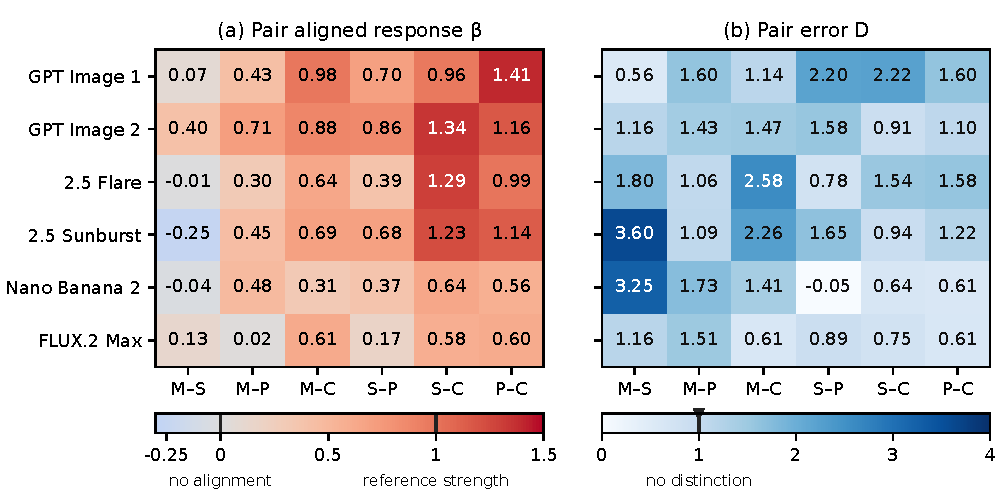
\includegraphics[width=\linewidth]{specificity_artist_pairs.pdf}
\caption{Descriptive painter-pair estimates (no pairwise tests). M, S, P and C denote Monet, Sisley,
Pissarro and C\'ezanne. Pair aligned response 0 means no aligned component,
1 matches reference strength, values above 1 exaggerate it, and negative values
indicate the opposite direction.
Expected error is 0 for exact agreement and 1 for no distinction. Each pair uses
all 31 features and is normalized by its squared reference distance.
Negative error can arise from repeat correction,
not better-than-exact agreement.}
\label{fig:artist-pairs}
\end{figure}
\FloatBarrier

\subsection{Detailed interpretation of the original comparisons}
\paragraph{A Response in the Right Direction Can Still Miss the Target}
All 1,008 outputs yield valid measurements. With the full-frame
reference target, every model's aligned-response interval lies above zero
(Appendix Table~\ref{tab:specificity-models}). A purely common additive response is
therefore insufficient to explain the named conditions under the stated
inference model. Yet positive alignment does not ensure low error. GPT Image 2
nearly matches the reference-aligned strength, $\beta=.999\;[.893,1.104]$,
while its total error is $D=1.226$: it adds substantial differences beyond
that aligned component.




FLUX.2 Max has the lowest error estimate, $.801$, despite a smaller aligned
response, $.470$. Adjusted comparisons resolve higher error for Flare and Sunburst
than for FLUX; the other 13 intervals include zero (Appendix~\ref{app:results},
Table~\ref{tab:all-specificity-pairs}).
These use full-frame references;
the Sunburst result changes after source correction
(Section~\ref{sec:source-correction}). No model is established to beat the
no-contrast benchmark of one. Thus the study detects a
reference-aligned response more clearly than it establishes low total mismatch.

Appendix~\ref{app:geometry} visualizes the same labeled contrasts in two
reference-fitted axes; Appendix Figure~\ref{fig:artist-pairs} uses all 31 features.



\paragraph{Uneven Painter Distinctions in the 31 Features}
Retrospective pair diagnostics extend the lightness example in
Section~\ref{sec:contrast-intuition} to all 31 features (Appendix Figure~\ref{fig:artist-pairs}).
Monet--Sisley aligned responses range from $-.249$ to $.129$ in five models,
versus $.402$ for GPT Image 2. Yet GPT Image 1 has lower estimated error for this pair
($.56$ versus $1.16$): stronger alignment does not ensure lower mismatch.
Omitting C\'ezanne lowers FLUX's overall response from $.470$ to $.096$ and
GPT Image 2's from $.999$ to $.651$.

Swapping Monet and Sisley lowers error for Flare, Sunburst and Nano Banana 2.
Reversing a negatively aligned pair difference lowers error without changing its size.




\paragraph{Which Comparisons Survive Reference Changes?}
Within the 31-feature metric, FLUX retains the lowest uncalibrated scene-error point
estimate across scene deletions, measurement windows, reference targets and
feature-weighting sensitivities (Appendices~\ref{app:declared-sensitivities}
and~\ref{app:diagnostics}).

Source handling has a more consequential effect on statistical comparisons.
AI assistants inspected all reference and development reproductions, selecting
crops that exclude peripheral artifacts in 90 reference and 41 development images.
The audit used no human verification. After cropping and refitting development scaling,
FLUX's error estimate changes from $.801$ to $.872$. Corrected aligned-response
intervals remain above zero for all six models, and GPT Image 2 retains the lowest
calibrated estimate.

Appendix Table~\ref{tab:source-comparison} makes the changed comparisons explicit. With
corrected regions and refitted scaling, the Sunburst interval crosses zero,
Flare still has higher error than FLUX and the GPT Image 1 interval moves above zero. The latter
is a retrospective sensitivity, not a new confirmatory finding. Source correction
preserves FLUX's lowest point estimate while changing the evidence for particular
model differences.
Weak Monet--Sisley alignment also persists after correction, but individual
signs are unstable: Flare changes from $-.011$ to $.019$, GPT Image 1 from
$.074$ to $-.053$, and FLUX from $.129$ to $.019$. The label-swap observation
above therefore concerns the original reference target.






A separate check uses class-specific reference means for 11 water, built and
land briefs, excluding three mixed briefs. Replacing title-derived reference
labels with visual labels retains FLUX's lowest error estimate.
Appendix~\ref{app:diagnostics} gives the controls and audit.\par




\FloatBarrier
\section{A Separate Matched-seed Collection}\label{app:cross-cohort}
This retrospective extension applies the common/centered decomposition to the
complete retained SD-Turbo collection from 5 September 2026. Its ordinary
feature-distance and coordinate diagnostics had already been analyzed; it is
not an untouched validation set. The present definitions, code and constructed
tests were fixed before calculating these new decomposition outcomes. The
2,000 original-image hashes are disjoint from the main 1,008-image collection,
and the exact prompt strings differ. The historical references and feature
scaler are shared, previously exposed finite targets.

\subsection{Census, prompts and paired seeds}
The complete design is 25 repeat blocks, 16 scenes and five prompt conditions,
with 400 outputs per condition. The baseline reads ``An oil painting on canvas
of \ldots''; each named arm inserts only `` by [painter]'' after ``canvas''.
All four painters remain. This baseline already contains a painting
instruction; it contains no Impressionist or shared-family clause.

The fixed checkpoint is \texttt{stabilityai/sd-turbo}. The recorded revision is
\begin{quote}\texttt{b261bac6fd2cf515557d5d0707481eafa0485ec2}.\end{quote}
Generation uses 512-square images, fp16 on Apple MPS, one denoising step,
guidance scale zero and no negative prompt.
The recorded collection ran from 00:38:02 to 02:02:39 UTC. Every output
has retained raw bytes and a complete 31-coordinate measurement; no model
rerun or new extraction is needed for this analysis.

Within each scene/block, all five arms use the same seed, with the generator
reset for every image. The 400 distinct scene/block seeds are derived by the
frozen HMAC rule. Hence artist conditions are deliberately paired. The repeat
unit is the complete 80-image block, not an individual condition. Stable
generation under distinct pseudo-random seed streams motivates the
cross-block interpretation below; it does not calibrate dependence in the
closed services of the main experiment.

\subsection{Cross-block quantities}
Use the retained development-panel coordinate center and IQR scale, with no
refitting. Let $z_{bsa}$ denote a standardized vector, $b=1,\ldots,25$,
$s=1,\ldots,16$, $a=0$ for the painting baseline and $a=1,\ldots,4$ for names.
For block vectors $v_b$, define
\begin{equation}
 U_K(v)=\frac{\|\sum_b v_b\|^2-\sum_b\|v_b\|^2}{K(K-1)}
       =\frac{1}{K(K-1)}\sum_{b\ne b'}v_b^\top v_{b'}.
\end{equation}
This is the average cross-product over distinct repeat blocks. Under stable
means and independent mean-zero block errors it estimates the squared mean
response; arbitrary covariance among arms within a block is allowed.
Signed finite-sample values are retained.

First average scenes within each block and define
\begin{align}
 \delta_{ba}&=\tfrac1{16}\sum_s(z_{bsa}-z_{bs0}),&
 c_b&=\tfrac14\sum_a\delta_{ba},& d_{ba}&=\delta_{ba}-c_b,\\
 C&=4U_K(c),& L&=\sum_a U_K(d_a),& N&=\sum_a U_K(\delta_a)=C+L.
\end{align}
The descriptive common-majority criterion is $N>0$ and $T=C-L>0$.
The ratio $C/N$ is reported only for $N>0$, without clipping either components
or ratios. A within-scene version computes components before averaging the
16 scalar results. It is a separate target, not an alternative selected for
a favorable answer. All 31 coordinates are primary; the fixed color, spatial
and texture families are mandatory sensitivities.

Let $r_a$ be centered historical painter means and $H=\sum_a\|r_a\|^2$.
The pooled context quantities are
\begin{equation}
 \beta=H^{-1}\sum_a\langle\bar d_a,r_a\rangle,\qquad
 D_{\rm pooled}=H^{-1}\sum_a U_K(d_a-r_a)
              =L/H-2\beta+1.
\end{equation}
Scene-wise error instead applies the cross-block calculation before averaging
scenes. Both are retained. Each feature family uses its own restricted $H$;
zero historical energy makes normalized quantities unavailable. All six pair
amplitudes and scene-wise errors use the corresponding historical squared
pair distance. The code checks the component and error identities directly.

Deleting each block once leaves $K=24$ and recomputes every reported quantity,
with historical means and scaling unchanged. The 25 deletion values and their
ranges describe sensitivity. They are not confidence intervals or new
confirmatory tests. This separate collection changes model, template,
resolution and generation mechanism together; it does not identify which
change causes any difference, validate a shared-family interpretation, or
establish perceptual fidelity.

% Generated from frozen retrospective SD-Turbo results; no new analysis.
% analysis_sha256: 9488dfafa5779b8b065cc756804e67ad64c2841a5c62c2f9b0105f8fef13973e
% inputs_sha256: 94413b3ee5bd689f60df35e7a8135f79eb929fd9dbee36bd450b47df4db0e693
\subsection{Complete separate-collection summaries}
\begin{table}[!htbp]
\caption{All fixed SD-Turbo decomposition summaries. Pooled averages each condition over the 16 scenes before cross-block products; within scene averages the resulting 16 scalar summaries. $C$ is common additional naming change beyond generic oil painting, $L$ is centered between-name change, $N=C+L$ and $T=C-L$. Positive $N$ and $T$ define a descriptive common majority. Texture fails this criterion under both targets. The ratio, alignment $\beta$ and normalized error $D$ retain their signed values; none is a perceptual-fidelity score.}
\label{tab:cross-cohort-components}
\centering\small\setlength{\tabcolsep}{4pt}
\begin{tabularx}{\linewidth}{@{}Xlrrrrrrr@{}}\toprule
Coordinates & Target & $C$ & $L$ & $N$ & $T$ & $C/N$ & $\beta$ & $D$\\\midrule
All 31 & Pooled & $12.212$ & $6.814$ & $19.026$ & $5.397$ & $0.642$ & $0.618$ & $0.917$\\
All 31 & Within scene & $28.993$ & $11.071$ & $40.064$ & $17.922$ & $0.724$ & $0.618$ & $1.637$\\
\addlinespace[2pt]
Color (11) & Pooled & $2.753$ & $2.034$ & $4.787$ & $0.719$ & $0.575$ & $0.632$ & $0.692$\\
Color (11) & Within scene & $4.881$ & $2.442$ & $7.323$ & $2.438$ & $0.666$ & $0.632$ & $0.884$\\
\addlinespace[2pt]
Spatial (8) & Pooled & $7.471$ & $1.334$ & $8.805$ & $6.137$ & $0.849$ & $0.310$ & $1.270$\\
Spatial (8) & Within scene & $20.442$ & $4.732$ & $25.175$ & $15.710$ & $0.812$ & $0.310$ & $3.539$\\
\addlinespace[2pt]
Texture (12) & Pooled & $1.988$ & $3.446$ & $5.434$ & $-1.459$ & $0.366$ & $0.805$ & $0.895$\\
Texture (12) & Within scene & $3.670$ & $3.896$ & $7.566$ & $-0.226$ & $0.485$ & $0.805$ & $1.091$\\
\bottomrule\end{tabularx}\end{table}
The fixed historical reference energy $H$ is All 31: $5.915007$, Color (11): $2.126435$, Spatial (8): $1.498037$, Texture (12): $2.290536$.
The signed within-scene minus pooled $D$ difference is All 31: $0.719664$, Color (11): $0.191996$, Spatial (8): $2.268590$, Texture (12): $0.196511$.
\begin{table}[!htbp]
\caption{All six painter pairs in every coordinate view. Pair denominator $H_{aj}=\|\mu_a-\mu_j\|^2$ uses that view's historical means. Aligned amplitude is $\langle\overline{z_a-z_j},\mu_a-\mu_j\rangle/H_{aj}$. Pair $D_{\rm scene}$ averages cross-block squared-error estimates within scenes and divides by $H_{aj}$. Negative amplitudes are retained. No pair hypothesis tests or perceptual-fidelity claims are made.}
\label{tab:cross-cohort-pairs}
\centering\small\setlength{\tabcolsep}{4pt}
\begin{tabularx}{\linewidth}{@{}lXrrr@{}}\toprule
Coordinates & Pair & $H_{aj}$ & Amplitude & $D_{\rm scene}$\\\midrule
All 31 & Monet--Sisley & $1.972$ & $0.471$ & $3.319$\\
All 31 & Monet--Pissarro & $2.404$ & $0.494$ & $1.912$\\
All 31 & Monet--C\'ezanne & $6.113$ & $0.871$ & $1.367$\\
All 31 & Sisley--Pissarro & $1.665$ & $0.224$ & $2.612$\\
All 31 & Sisley--C\'ezanne & $5.256$ & $0.625$ & $1.624$\\
All 31 & Pissarro--C\'ezanne & $6.250$ & $0.563$ & $1.014$\\
\addlinespace[3pt]
Color (11) & Monet--Sisley & $0.383$ & $0.100$ & $1.934$\\
Color (11) & Monet--Pissarro & $0.626$ & $0.321$ & $1.675$\\
Color (11) & Monet--C\'ezanne & $2.434$ & $0.754$ & $0.734$\\
Color (11) & Sisley--Pissarro & $0.285$ & $0.166$ & $4.184$\\
Color (11) & Sisley--C\'ezanne & $2.311$ & $0.814$ & $0.456$\\
Color (11) & Pissarro--C\'ezanne & $2.466$ & $0.558$ & $0.689$\\
\addlinespace[3pt]
Spatial (8) & Monet--Sisley & $0.230$ & $-0.523$ & $22.882$\\
Spatial (8) & Monet--Pissarro & $1.189$ & $0.437$ & $2.303$\\
Spatial (8) & Monet--C\'ezanne & $1.186$ & $0.227$ & $3.543$\\
Spatial (8) & Sisley--Pissarro & $0.583$ & $0.725$ & $3.266$\\
Spatial (8) & Sisley--C\'ezanne & $1.424$ & $0.187$ & $3.273$\\
Spatial (8) & Pissarro--C\'ezanne & $1.380$ & $0.362$ & $1.765$\\
\addlinespace[3pt]
Texture (12) & Monet--Sisley & $1.359$ & $0.743$ & $0.399$\\
Texture (12) & Monet--Pissarro & $0.589$ & $0.793$ & $1.373$\\
Texture (12) & Monet--C\'ezanne & $2.492$ & $1.292$ & $0.950$\\
Texture (12) & Sisley--Pissarro & $0.797$ & $-0.123$ & $1.572$\\
Texture (12) & Sisley--C\'ezanne & $1.522$ & $0.747$ & $1.856$\\
Texture (12) & Pissarro--C\'ezanne & $2.404$ & $0.682$ & $0.916$\\
\bottomrule\end{tabularx}\end{table}
\FloatBarrier
\begin{table}[!htbp]
\caption{Finite ranges over all 25 delete-one-block analyses for the unnormalized components. Each recomputation uses the remaining $K=24$ complete paired-seed blocks and all 16 scenes. These are stability ranges, not confidence intervals. All 25 values enter each displayed range; negative texture contrasts remain negative.}
\label{tab:cross-cohort-delete-energy}
\centering\small\setlength{\tabcolsep}{4pt}
\begin{tabularx}{\linewidth}{@{}Xlrrrr@{}}\toprule
Coordinates & Target & $C$ & $L$ & $N$ & $T$\\\midrule
All 31 & Pooled & $[12.003, 12.415]$ & $[6.785, 6.898]$ & $[18.792, 19.261]$ & $[5.215, 5.610]$\\
All 31 & Within scene & $[28.063, 29.673]$ & $[10.982, 11.187]$ & $[39.116, 40.860]$ & $[17.009, 18.486]$\\
\addlinespace[2pt]
Color (11) & Pooled & $[2.730, 2.786]$ & $[2.023, 2.050]$ & $[4.756, 4.819]$ & $[0.693, 0.752]$\\
Color (11) & Within scene & $[4.813, 4.956]$ & $[2.429, 2.459]$ & $[7.242, 7.397]$ & $[2.385, 2.514]$\\
\addlinespace[2pt]
Spatial (8) & Pooled & $[7.263, 7.664]$ & $[1.316, 1.363]$ & $[8.593, 9.010]$ & $[5.917, 6.343]$\\
Spatial (8) & Within scene & $[19.525, 21.119]$ & $[4.663, 4.833]$ & $[24.257, 25.953]$ & $[14.793, 16.286]$\\
\addlinespace[2pt]
Texture (12) & Pooled & $[1.955, 2.012]$ & $[3.419, 3.493]$ & $[5.384, 5.492]$ & $[-1.497, -1.422]$\\
Texture (12) & Within scene & $[3.621, 3.717]$ & $[3.868, 3.937]$ & $[7.498, 7.606]$ & $[-0.269, -0.164]$\\
\bottomrule\end{tabularx}\end{table}
\begin{table}[!htbp]
\caption{Finite ranges over the same complete 25 delete-one-block analyses for normalized summaries. The 649-work historical target, 221-work development scaling and view-specific denominators stay fixed. Every displayed range uses all 25 values. These ranges quantify deletion sensitivity and provide no coverage guarantee.}
\label{tab:cross-cohort-delete-normalized}
\centering\small\setlength{\tabcolsep}{4pt}
\begin{tabularx}{\linewidth}{@{}Xlrrr@{}}\toprule
Coordinates & Target & $C/N$ & $\beta$ & $D$\\\midrule
All 31 & Pooled & $[0.639, 0.646]$ & $[0.615, 0.620]$ & $[0.910, 0.929]$\\
All 31 & Within scene & $[0.717, 0.727]$ & $[0.615, 0.620]$ & $[1.621, 1.655]$\\
\addlinespace[2pt]
Color (11) & Pooled & $[0.573, 0.578]$ & $[0.628, 0.636]$ & $[0.688, 0.696]$\\
Color (11) & Within scene & $[0.664, 0.670]$ & $[0.628, 0.636]$ & $[0.881, 0.888]$\\
\addlinespace[2pt]
Spatial (8) & Pooled & $[0.844, 0.853]$ & $[0.304, 0.319]$ & $[1.249, 1.297]$\\
Spatial (8) & Within scene & $[0.805, 0.815]$ & $[0.304, 0.319]$ & $[3.491, 3.610]$\\
\addlinespace[2pt]
Texture (12) & Pooled & $[0.362, 0.369]$ & $[0.802, 0.810]$ & $[0.889, 0.906]$\\
Texture (12) & Within scene & $[0.482, 0.489]$ & $[0.802, 0.810]$ & $[1.083, 1.104]$\\
\bottomrule\end{tabularx}\end{table}
\FloatBarrier
The retained numeric record includes all 25 individual deletion results, all 16 scene records and full-precision endpoints. These generated tables are checked by \texttt{python paper/make\_icml\_cross\_cohort\_tables.py --check}; the check verifies frozen hashes and recomputes every displayed range from the complete deletion inventory.

\FloatBarrier
\section{Reference-calibrated Attribution with Abstention}\label{app:selective}
This retrospective test asks when an existing reference-prototype assignment
should be issued rather than withheld. Its rule is fixed using historical
artworks; no generated prompt label fits or tunes the gate. The same generated
images and their earlier baseline confusions were previously inspected, so
the experiment is not independent confirmation. The primary condition is CSD
with original primary prototypes. Both encoders and every original/audited
view and primary/development prototype target remain mandatory outputs.

\subsection{Fixed calibration and decision rule}
Use the same unit-normalized historical prototype directions $u_a$ as the
existing baseline. The other historical partition supplies calibration:
development works for primary prototypes, primary works for development
prototypes. The selected source view is used consistently in both partitions;
an audited crop replaces only the previously declared region of that work.

For a calibration artwork $x$ labeled $a$, define nonconformity
\begin{equation}
 s_a(x)=\max_{b\ne a}x^\top u_b-x^\top u_a.
\end{equation}
With $n_a$ calibration works for painter $a$, set
$k_a=\lceil(n_a+1)(1-.10)\rceil$ and take $q_a$ to be the $k_a$-th smallest
score, using $+\infty$ when $k_a>n_a$. There is no interpolated quantile or
alternative nominal level. For each generated query form
\begin{equation}
 C(x)=\{a:s_a(x)\le q_a\},\qquad
 \hat a(x)=\arg\max_a x^\top u_a.
\end{equation}
Issue the unchanged top-1 assignment only if $C(x)=\{\hat a(x)\}$.
Otherwise abstain, retaining empty, multiple-label and disagreeing-singleton
sets as separate reasons. Ties in top-1 follow the fixed painter order.

This uses an ordinary rank-calibration rule as an empirical diagnostic.
Exchangeability between historical art and generated images is not established;
the numerical $.10$ choice is not a guarantee of generated-image coverage or
selective error. No density-ratio correction or shift assumption from
\citet{tibshirani2019shift} is fitted. The general rejection/coverage tradeoff
is established work \citep{geifman2017selective}, not an algorithmic novelty.

\subsection{Coverage-matched comparison and operational criterion}
Within a configuration's 112 named queries, let $K$ be the number accepted by
the reference gate. The comparator keeps exactly the $K$ greatest top-two
prototype margins, breaking ties by frozen observation ID. It uses no true
prompt name in selection. This is a transductive descriptive comparator: its
cutoff uses the query distribution, whereas the reference gate's thresholds
use historical artworks. Predictions remain the original top-1 assignments.
For controls, apply the resulting numeric margin cutoff inclusively, retaining
boundary ties. If $K=0$, neither named queries nor controls are accepted; if
$K=112$, the minimum named margin is still the cutoff for controls. No prompt
label determines either selection rule.

The pre-outcome operational criterion requires at least 50\% named-image
coverage in every configuration, at least one accepted query from every
prompted painter in each configuration, and positive equal-configuration mean
reductions in accepted error relative to both unrestricted top-1 and the
coverage-matched comparator. These joint descriptive conditions prevent a
nearly empty accepted set from being credited as useful. Undefined accepted
error is retained as a failure, without dropping its configuration from an
otherwise favorable mean. All individual adverse results remain visible.
The 50\% threshold is this study's declared operating requirement, not a
universal criterion for useful selective classification.

For every encoder/view/target/configuration, retain the individual scores,
candidate sets, predictions, decisions, painter-specific coverage, accepted
and abstained error, and correct/incorrect counts. Delete each scene once to
describe sensitivity, without changing historical calibration or interpreting
the ranges as sampling intervals. Control-arm results report name-assignment
rates separately for artist-free and generic-painting images. These rates
concern assignments without a candidate name in the prompt; they do not
establish that such an image has no resemblance to that painter.

% Generated by paper/make_icml_selective_tables.py; retained outcomes only.
% analysis_sha256: f725b32b91f38fa8afd85454b3a6f0c8eb7464f5337b18373ce8c8f53e39fa2c
% inputs_sha256: f9d6b94e19d8004463f7b0524dd72865e22c18b0786cf48387cb9257e0528826
% audit_sha256: e3f26efb7286ad592e5ec30a50dd937690c29852d690c94b3baf09f31ae22569
% generator_sha256: 36191527ea108614a42cd949af9f3cdfbc16b01df7216fd40191198936079ec1
\clearpage\subsection{Complete selective-attribution results}
\label{app:selective-results}
The primary CSD/original/primary setting and all seven sensitivities are retained. A denotes the fixed reference gate and M the coverage-matched ordinary-margin comparator. All error rates concern recorded prompt names. These retrospective decisions do not establish perceptual fidelity, a generated-image coverage guarantee or independent replication.
\subsection{Joint operational criteria and aggregate influence}
C1 requires at least 50\% named-image coverage in every configuration. C2 requires at least one accepted image from every prompted painter in every configuration. C3 and C4 require strictly positive equal-configuration mean error reductions against unrestricted top-1 and the coverage-matched margin comparator, respectively. All four must pass. An undefined mean fails its criterion; it is never computed from a subset of configurations.
\begin{table}[!htbp]
\caption{All fixed criteria. O/A denote original/audited reference views and P/D denote primary/development prototypes, with the other partition used for calibration. Mean reductions are percentage points; positive values favor the gate. Every setting fails its joint criterion. Missing means remain explicit.}
\label{tab:selective-criteria}
\centering\footnotesize\setlength{\tabcolsep}{3pt}
\begin{tabularx}{\linewidth}{@{}Xrrccccc@{}}\toprule
Setting & $B-A$ & $M-A$ & C1 & C2 & C3 & C4 & Missing\\\midrule
CLIP / O / P & $+12.06$ & $+1.66$ & Fail & Pass & Pass & Pass & 0\\
CLIP / O / D & $+17.26$ & $+2.80$ & Fail & Pass & Pass & Pass & 0\\
CLIP / A / P & $+14.52$ & $+0.26$ & Fail & Pass & Pass & Pass & 0\\
CLIP / A / D & $+17.35$ & $+3.12$ & Fail & Pass & Pass & Pass & 0\\
CSD / O / P & $+26.03$ & $+0.53$ & Fail & Fail & Pass & Pass & 0\\
CSD / O / D & $+27.76$ & $-0.07$ & Fail & Fail & Pass & Fail & 0\\
CSD / A / P & $+26.00$ & $+0.96$ & Fail & Fail & Pass & Pass & 0\\
CSD / A / D & $+25.66$ & $-2.30$ & Fail & Fail & Pass & Fail & 0\\
\bottomrule\end{tabularx}
\end{table}
\begin{table}[!htbp]
\caption{Equal-configuration ranges over all 14 scene deletions. Prototypes and gate thresholds remain fixed; the margin comparator is matched anew on the remaining queries. Coverage and accepted error are percentages; reductions are percentage points. These are influence ranges, not confidence intervals. U counts unavailable deletions for each of the four displayed quantities, in column order.}
\label{tab:selective-aggregate-influence}
\centering\footnotesize\setlength{\tabcolsep}{2pt}
\begin{tabularx}{\linewidth}{@{}Xrrrrl@{}}\toprule
Setting & Coverage & A error & $B-A$ & $M-A$ & U\\\midrule
CLIP / O / P & $[58.5, 63.0]$ & $[28.7, 32.2]$ & $[+10.86, +13.56]$ & $[+0.79, +2.54]$ & 0/0/0/0\\
CLIP / O / D & $[47.3, 51.3]$ & $[24.7, 27.6]$ & $[+16.46, +18.57]$ & $[+2.00, +3.58]$ & 0/0/0/0\\
CLIP / A / P & $[55.1, 59.8]$ & $[27.5, 30.4]$ & $[+13.00, +15.57]$ & $[-0.23, +1.10]$ & 0/0/0/0\\
CLIP / A / D & $[45.7, 49.4]$ & $[23.7, 26.3]$ & $[+16.66, +18.50]$ & $[+2.04, +3.53]$ & 0/0/0/0\\
CSD / O / P & $[34.3, 36.7]$ & $[12.4, 14.2]$ & $[+25.28, +26.89]$ & $[+0.21, +0.91]$ & 0/0/0/0\\
CSD / O / D & $[32.4, 34.5]$ & $[15.6, 17.7]$ & $[+26.95, +28.76]$ & $[-0.83, +1.61]$ & 0/0/0/0\\
CSD / A / P & $[34.0, 36.4]$ & $[12.6, 14.5]$ & $[+25.23, +27.30]$ & $[+0.40, +1.07]$ & 0/0/0/0\\
CSD / A / D & $[33.2, 35.1]$ & $[18.3, 20.2]$ & $[+24.66, +26.33]$ & $[-3.30, -1.38]$ & 0/0/0/0\\
\bottomrule\end{tabularx}
\end{table}
\FloatBarrier
\clearpage\subsection{Original sources / primary prototypes}
\begin{table}[!htbp]
\caption{Original sources / primary prototypes: complete coverage/error comparison. $K$ is accepted named queries out of 112. B is unrestricted error; A and M are accepted error for the reference gate and exact-coverage margin comparator. Rates are percentages and differences are percentage points. Negative differences and undefined risks (--) are retained.}
\label{tab:selective-risks-original-primary}
\centering\footnotesize\setlength{\tabcolsep}{3pt}
\begin{tabularx}{\linewidth}{@{}Xlrrrrrrr@{}}\toprule
Configuration & Encoder & $K$ & Coverage & B & A & M & $B-A$ & $M-A$\\\midrule
GPT Image 1 & CLIP & 55 & $49.1$ & $39.3$ & $25.5$ & $25.5$ & $+13.83$ & $+0.00$\\
GPT Image 2 & CLIP & 71 & $63.4$ & $31.2$ & $21.1$ & $19.7$ & $+10.12$ & $-1.41$\\
GPT 2.5 Flare & CLIP & 62 & $55.4$ & $40.2$ & $25.8$ & $29.0$ & $+14.37$ & $+3.23$\\
GPT 2.5 Sunburst & CLIP & 59 & $52.7$ & $41.1$ & $18.6$ & $22.0$ & $+22.43$ & $+3.39$\\
Nano Banana 2 & CLIP & 83 & $74.1$ & $48.2$ & $38.6$ & $44.6$ & $+9.66$ & $+6.02$\\
FLUX.2 Max & CLIP & 79 & $70.5$ & $58.9$ & $57.0$ & $55.7$ & $+1.97$ & $-1.27$\\
GPT Image 1 & CSD & 30 & $26.8$ & $27.7$ & $0.0$ & $0.0$ & $+27.68$ & $+0.00$\\
GPT Image 2 & CSD & 37 & $33.0$ & $24.1$ & $2.7$ & $2.7$ & $+21.40$ & $+0.00$\\
GPT 2.5 Flare & CSD & 27 & $24.1$ & $37.5$ & $0.0$ & $0.0$ & $+37.50$ & $+0.00$\\
GPT 2.5 Sunburst & CSD & 30 & $26.8$ & $38.4$ & $0.0$ & $0.0$ & $+38.39$ & $+0.00$\\
Nano Banana 2 & CSD & 51 & $45.5$ & $49.1$ & $25.5$ & $33.3$ & $+23.62$ & $+7.84$\\
FLUX.2 Max & CSD & 64 & $57.1$ & $60.7$ & $53.1$ & $48.4$ & $+7.59$ & $-4.69$\\
\bottomrule\end{tabularx}
\end{table}
\begin{table}[!htbp]
\caption{Original sources / primary prototypes: painter retention and conditional error. Each painter cell is accepted count/28 (the coverage fraction), followed by $\mid$ accepted error in percent. -- denotes undefined error at zero acceptance, not zero error. The original CSD GPT Image 1 result accepts 28 C\'ezanne images, one Monet, one Pissarro and no Sisley; its zero aggregate accepted error therefore does not cover all four painter conditions.}
\label{tab:selective-painters-original-primary}
\centering\footnotesize\setlength{\tabcolsep}{2pt}
\begin{tabularx}{\linewidth}{@{}Xl*{4}{>{\centering\arraybackslash}p{.153\linewidth}}@{}}\toprule
Configuration & Encoder & Monet & Sisley & Pissarro & C\'ezanne\\\midrule
GPT Image 1 & CLIP & 6/28 $\mid$ $50.0$ & 13/28 $\mid$ $61.5$ & 13/28 $\mid$ $23.1$ & 23/28 $\mid$ $0.0$\\
GPT Image 2 & CLIP & 13/28 $\mid$ $23.1$ & 15/28 $\mid$ $46.7$ & 17/28 $\mid$ $29.4$ & 26/28 $\mid$ $0.0$\\
GPT 2.5 Flare & CLIP & 9/28 $\mid$ $55.6$ & 16/28 $\mid$ $50.0$ & 11/28 $\mid$ $27.3$ & 26/28 $\mid$ $0.0$\\
GPT 2.5 Sunburst & CLIP & 6/28 $\mid$ $50.0$ & 12/28 $\mid$ $25.0$ & 14/28 $\mid$ $35.7$ & 27/28 $\mid$ $0.0$\\
Nano Banana 2 & CLIP & 12/28 $\mid$ $100.0$ & 23/28 $\mid$ $52.2$ & 22/28 $\mid$ $36.4$ & 26/28 $\mid$ $0.0$\\
FLUX.2 Max & CLIP & 16/28 $\mid$ $100.0$ & 24/28 $\mid$ $75.0$ & 20/28 $\mid$ $20.0$ & 19/28 $\mid$ $36.8$\\
GPT Image 1 & CSD & 1/28 $\mid$ $0.0$ & 0/28 $\mid$ -- & 1/28 $\mid$ $0.0$ & 28/28 $\mid$ $0.0$\\
GPT Image 2 & CSD & 1/28 $\mid$ $0.0$ & 1/28 $\mid$ $100.0$ & 8/28 $\mid$ $0.0$ & 27/28 $\mid$ $0.0$\\
GPT 2.5 Flare & CSD & 0/28 $\mid$ -- & 0/28 $\mid$ -- & 2/28 $\mid$ $0.0$ & 25/28 $\mid$ $0.0$\\
GPT 2.5 Sunburst & CSD & 0/28 $\mid$ -- & 0/28 $\mid$ -- & 2/28 $\mid$ $0.0$ & 28/28 $\mid$ $0.0$\\
Nano Banana 2 & CSD & 6/28 $\mid$ $100.0$ & 9/28 $\mid$ $77.8$ & 8/28 $\mid$ $0.0$ & 28/28 $\mid$ $0.0$\\
FLUX.2 Max & CSD & 8/28 $\mid$ $100.0$ & 17/28 $\mid$ $100.0$ & 22/28 $\mid$ $0.0$ & 17/28 $\mid$ $52.9$\\
\bottomrule\end{tabularx}
\end{table}
\begin{table}[!htbp]
\caption{Original sources / primary prototypes: control-arm named-attribution rates. Each entry is accepted count/28 and percentage. A is the reference gate; M uses the named pool's numeric margin cutoff inclusively, without splitting control ties. These prompts contain no candidate artist name; acceptance is not evidence of a human-perceived style error.}
\label{tab:selective-controls-original-primary}
\centering\footnotesize\setlength{\tabcolsep}{3pt}
\begin{tabularx}{\linewidth}{@{}Xlrrrr@{}}\toprule
Configuration & Encoder & Free A & Free M & Generic A & Generic M\\\midrule
GPT Image 1 & CLIP & 6/28 ($21.4$) & 6/28 ($21.4$) & 8/28 ($28.6$) & 4/28 ($14.3$)\\
GPT Image 2 & CLIP & 7/28 ($25.0$) & 8/28 ($28.6$) & 11/28 ($39.3$) & 10/28 ($35.7$)\\
GPT 2.5 Flare & CLIP & 5/28 ($17.9$) & 7/28 ($25.0$) & 7/28 ($25.0$) & 8/28 ($28.6$)\\
GPT 2.5 Sunburst & CLIP & 6/28 ($21.4$) & 5/28 ($17.9$) & 5/28 ($17.9$) & 6/28 ($21.4$)\\
Nano Banana 2 & CLIP & 4/28 ($14.3$) & 8/28 ($28.6$) & 8/28 ($28.6$) & 17/28 ($60.7$)\\
FLUX.2 Max & CLIP & 5/28 ($17.9$) & 10/28 ($35.7$) & 13/28 ($46.4$) & 20/28 ($71.4$)\\
GPT Image 1 & CSD & 14/28 ($50.0$) & 5/28 ($17.9$) & 9/28 ($32.1$) & 8/28 ($28.6$)\\
GPT Image 2 & CSD & 7/28 ($25.0$) & 4/28 ($14.3$) & 7/28 ($25.0$) & 7/28 ($25.0$)\\
GPT 2.5 Flare & CSD & 4/28 ($14.3$) & 0/28 ($0.0$) & 6/28 ($21.4$) & 2/28 ($7.1$)\\
GPT 2.5 Sunburst & CSD & 4/28 ($14.3$) & 0/28 ($0.0$) & 5/28 ($17.9$) & 2/28 ($7.1$)\\
Nano Banana 2 & CSD & 14/28 ($50.0$) & 5/28 ($17.9$) & 17/28 ($60.7$) & 11/28 ($39.3$)\\
FLUX.2 Max & CSD & 13/28 ($46.4$) & 8/28 ($28.6$) & 21/28 ($75.0$) & 21/28 ($75.0$)\\
\bottomrule\end{tabularx}
\end{table}
\FloatBarrier
\clearpage\subsection{Original sources / development prototypes}
\begin{table}[!htbp]
\caption{Original sources / development prototypes: complete coverage/error comparison. $K$ is accepted named queries out of 112. B is unrestricted error; A and M are accepted error for the reference gate and exact-coverage margin comparator. Rates are percentages and differences are percentage points. Negative differences and undefined risks (--) are retained.}
\label{tab:selective-risks-original-development}
\centering\footnotesize\setlength{\tabcolsep}{3pt}
\begin{tabularx}{\linewidth}{@{}Xlrrrrrrr@{}}\toprule
Configuration & Encoder & $K$ & Coverage & B & A & M & $B-A$ & $M-A$\\\midrule
GPT Image 1 & CLIP & 52 & $46.4$ & $39.3$ & $19.2$ & $25.0$ & $+20.05$ & $+5.77$\\
GPT Image 2 & CLIP & 58 & $51.8$ & $35.7$ & $19.0$ & $17.2$ & $+16.75$ & $-1.72$\\
GPT 2.5 Flare & CLIP & 54 & $48.2$ & $39.3$ & $16.7$ & $24.1$ & $+22.62$ & $+7.41$\\
GPT 2.5 Sunburst & CLIP & 54 & $48.2$ & $39.3$ & $22.2$ & $25.9$ & $+17.06$ & $+3.70$\\
Nano Banana 2 & CLIP & 60 & $53.6$ & $50.0$ & $30.0$ & $31.7$ & $+20.00$ & $+1.67$\\
FLUX.2 Max & CLIP & 54 & $48.2$ & $58.9$ & $51.9$ & $51.9$ & $+7.08$ & $+0.00$\\
GPT Image 1 & CSD & 37 & $33.0$ & $39.3$ & $5.4$ & $8.1$ & $+33.88$ & $+2.70$\\
GPT Image 2 & CSD & 30 & $26.8$ & $33.0$ & $0.0$ & $0.0$ & $+33.04$ & $+0.00$\\
GPT 2.5 Flare & CSD & 29 & $25.9$ & $40.2$ & $3.4$ & $3.4$ & $+36.73$ & $+0.00$\\
GPT 2.5 Sunburst & CSD & 39 & $34.8$ & $43.8$ & $15.4$ & $15.4$ & $+28.37$ & $+0.00$\\
Nano Banana 2 & CSD & 48 & $42.9$ & $55.4$ & $29.2$ & $33.3$ & $+26.19$ & $+4.17$\\
FLUX.2 Max & CSD & 41 & $36.6$ & $57.1$ & $48.8$ & $41.5$ & $+8.36$ & $-7.32$\\
\bottomrule\end{tabularx}
\end{table}
\begin{table}[!htbp]
\caption{Original sources / development prototypes: painter retention and conditional error. Each cell is accepted count/28 (coverage fraction), followed by $\mid$ accepted error in percent. -- denotes undefined error at zero acceptance, not zero error.}
\label{tab:selective-painters-original-development}
\centering\footnotesize\setlength{\tabcolsep}{2pt}
\begin{tabularx}{\linewidth}{@{}Xl*{4}{>{\centering\arraybackslash}p{.153\linewidth}}@{}}\toprule
Configuration & Encoder & Monet & Sisley & Pissarro & C\'ezanne\\\midrule
GPT Image 1 & CLIP & 7/28 $\mid$ $28.6$ & 9/28 $\mid$ $22.2$ & 10/28 $\mid$ $60.0$ & 26/28 $\mid$ $0.0$\\
GPT Image 2 & CLIP & 7/28 $\mid$ $14.3$ & 13/28 $\mid$ $0.0$ & 11/28 $\mid$ $81.8$ & 27/28 $\mid$ $3.7$\\
GPT 2.5 Flare & CLIP & 6/28 $\mid$ $33.3$ & 11/28 $\mid$ $0.0$ & 9/28 $\mid$ $77.8$ & 28/28 $\mid$ $0.0$\\
GPT 2.5 Sunburst & CLIP & 5/28 $\mid$ $40.0$ & 10/28 $\mid$ $0.0$ & 12/28 $\mid$ $83.3$ & 27/28 $\mid$ $0.0$\\
Nano Banana 2 & CLIP & 9/28 $\mid$ $100.0$ & 14/28 $\mid$ $28.6$ & 11/28 $\mid$ $45.5$ & 26/28 $\mid$ $0.0$\\
FLUX.2 Max & CLIP & 9/28 $\mid$ $100.0$ & 14/28 $\mid$ $50.0$ & 12/28 $\mid$ $41.7$ & 19/28 $\mid$ $36.8$\\
GPT Image 1 & CSD & 0/28 $\mid$ -- & 7/28 $\mid$ $0.0$ & 2/28 $\mid$ $100.0$ & 28/28 $\mid$ $0.0$\\
GPT Image 2 & CSD & 1/28 $\mid$ $0.0$ & 2/28 $\mid$ $0.0$ & 0/28 $\mid$ -- & 27/28 $\mid$ $0.0$\\
GPT 2.5 Flare & CSD & 0/28 $\mid$ -- & 3/28 $\mid$ $0.0$ & 1/28 $\mid$ $100.0$ & 25/28 $\mid$ $0.0$\\
GPT 2.5 Sunburst & CSD & 2/28 $\mid$ $100.0$ & 5/28 $\mid$ $0.0$ & 4/28 $\mid$ $100.0$ & 28/28 $\mid$ $0.0$\\
Nano Banana 2 & CSD & 8/28 $\mid$ $100.0$ & 7/28 $\mid$ $85.7$ & 5/28 $\mid$ $0.0$ & 28/28 $\mid$ $0.0$\\
FLUX.2 Max & CSD & 4/28 $\mid$ $100.0$ & 9/28 $\mid$ $100.0$ & 14/28 $\mid$ $0.0$ & 14/28 $\mid$ $50.0$\\
\bottomrule\end{tabularx}
\end{table}
\begin{table}[!htbp]
\caption{Original sources / development prototypes: control-arm named-attribution rates. Each entry is accepted count/28 and percentage. A is the reference gate; M uses the named pool's numeric margin cutoff inclusively, without splitting control ties. These prompts contain no candidate artist name; acceptance is not evidence of a human-perceived style error.}
\label{tab:selective-controls-original-development}
\centering\footnotesize\setlength{\tabcolsep}{3pt}
\begin{tabularx}{\linewidth}{@{}Xlrrrr@{}}\toprule
Configuration & Encoder & Free A & Free M & Generic A & Generic M\\\midrule
GPT Image 1 & CLIP & 11/28 ($39.3$) & 4/28 ($14.3$) & 7/28 ($25.0$) & 1/28 ($3.6$)\\
GPT Image 2 & CLIP & 9/28 ($32.1$) & 7/28 ($25.0$) & 7/28 ($25.0$) & 6/28 ($21.4$)\\
GPT 2.5 Flare & CLIP & 9/28 ($32.1$) & 5/28 ($17.9$) & 3/28 ($10.7$) & 1/28 ($3.6$)\\
GPT 2.5 Sunburst & CLIP & 10/28 ($35.7$) & 4/28 ($14.3$) & 4/28 ($14.3$) & 4/28 ($14.3$)\\
Nano Banana 2 & CLIP & 6/28 ($21.4$) & 4/28 ($14.3$) & 5/28 ($17.9$) & 5/28 ($17.9$)\\
FLUX.2 Max & CLIP & 7/28 ($25.0$) & 5/28 ($17.9$) & 6/28 ($21.4$) & 8/28 ($28.6$)\\
GPT Image 1 & CSD & 9/28 ($32.1$) & 7/28 ($25.0$) & 11/28 ($39.3$) & 11/28 ($39.3$)\\
GPT Image 2 & CSD & 3/28 ($10.7$) & 1/28 ($3.6$) & 3/28 ($10.7$) & 4/28 ($14.3$)\\
GPT 2.5 Flare & CSD & 1/28 ($3.6$) & 0/28 ($0.0$) & 4/28 ($14.3$) & 3/28 ($10.7$)\\
GPT 2.5 Sunburst & CSD & 1/28 ($3.6$) & 0/28 ($0.0$) & 3/28 ($10.7$) & 2/28 ($7.1$)\\
Nano Banana 2 & CSD & 6/28 ($21.4$) & 7/28 ($25.0$) & 12/28 ($42.9$) & 12/28 ($42.9$)\\
FLUX.2 Max & CSD & 10/28 ($35.7$) & 8/28 ($28.6$) & 22/28 ($78.6$) & 23/28 ($82.1$)\\
\bottomrule\end{tabularx}
\end{table}
\FloatBarrier
\clearpage\subsection{Audited regions / primary prototypes}
\begin{table}[!htbp]
\caption{Audited regions / primary prototypes: complete coverage/error comparison. $K$ is accepted named queries out of 112. B is unrestricted error; A and M are accepted error for the reference gate and exact-coverage margin comparator. Rates are percentages and differences are percentage points. Negative differences and undefined risks (--) are retained.}
\label{tab:selective-risks-audited-region-primary}
\centering\footnotesize\setlength{\tabcolsep}{3pt}
\begin{tabularx}{\linewidth}{@{}Xlrrrrrrr@{}}\toprule
Configuration & Encoder & $K$ & Coverage & B & A & M & $B-A$ & $M-A$\\\midrule
GPT Image 1 & CLIP & 51 & $45.5$ & $40.2$ & $21.6$ & $19.6$ & $+18.61$ & $-1.96$\\
GPT Image 2 & CLIP & 69 & $61.6$ & $30.4$ & $18.8$ & $17.4$ & $+11.52$ & $-1.45$\\
GPT 2.5 Flare & CLIP & 62 & $55.4$ & $42.9$ & $24.2$ & $27.4$ & $+18.66$ & $+3.23$\\
GPT 2.5 Sunburst & CLIP & 57 & $50.9$ & $40.2$ & $15.8$ & $17.5$ & $+24.39$ & $+1.75$\\
Nano Banana 2 & CLIP & 73 & $65.2$ & $50.0$ & $39.7$ & $41.1$ & $+10.27$ & $+1.37$\\
FLUX.2 Max & CLIP & 73 & $65.2$ & $59.8$ & $56.2$ & $54.8$ & $+3.66$ & $-1.37$\\
GPT Image 1 & CSD & 29 & $25.9$ & $26.8$ & $0.0$ & $0.0$ & $+26.79$ & $+0.00$\\
GPT Image 2 & CSD & 36 & $32.1$ & $24.1$ & $2.8$ & $2.8$ & $+21.33$ & $+0.00$\\
GPT 2.5 Flare & CSD & 27 & $24.1$ & $38.4$ & $0.0$ & $0.0$ & $+38.39$ & $+0.00$\\
GPT 2.5 Sunburst & CSD & 30 & $26.8$ & $39.3$ & $0.0$ & $0.0$ & $+39.29$ & $+0.00$\\
Nano Banana 2 & CSD & 52 & $46.4$ & $49.1$ & $28.8$ & $34.6$ & $+20.26$ & $+5.77$\\
FLUX.2 Max & CSD & 63 & $56.2$ & $60.7$ & $50.8$ & $50.8$ & $+9.92$ & $+0.00$\\
\bottomrule\end{tabularx}
\end{table}
\begin{table}[!htbp]
\caption{Audited regions / primary prototypes: painter retention and conditional error. Each cell is accepted count/28 (coverage fraction), followed by $\mid$ accepted error in percent. -- denotes undefined error at zero acceptance, not zero error.}
\label{tab:selective-painters-audited-region-primary}
\centering\footnotesize\setlength{\tabcolsep}{2pt}
\begin{tabularx}{\linewidth}{@{}Xl*{4}{>{\centering\arraybackslash}p{.153\linewidth}}@{}}\toprule
Configuration & Encoder & Monet & Sisley & Pissarro & C\'ezanne\\\midrule
GPT Image 1 & CLIP & 5/28 $\mid$ $40.0$ & 10/28 $\mid$ $50.0$ & 14/28 $\mid$ $28.6$ & 22/28 $\mid$ $0.0$\\
GPT Image 2 & CLIP & 12/28 $\mid$ $16.7$ & 14/28 $\mid$ $42.9$ & 17/28 $\mid$ $29.4$ & 26/28 $\mid$ $0.0$\\
GPT 2.5 Flare & CLIP & 9/28 $\mid$ $55.6$ & 16/28 $\mid$ $37.5$ & 12/28 $\mid$ $33.3$ & 25/28 $\mid$ $0.0$\\
GPT 2.5 Sunburst & CLIP & 5/28 $\mid$ $40.0$ & 11/28 $\mid$ $9.1$ & 14/28 $\mid$ $42.9$ & 27/28 $\mid$ $0.0$\\
Nano Banana 2 & CLIP & 11/28 $\mid$ $100.0$ & 20/28 $\mid$ $45.0$ & 17/28 $\mid$ $52.9$ & 25/28 $\mid$ $0.0$\\
FLUX.2 Max & CLIP & 16/28 $\mid$ $100.0$ & 22/28 $\mid$ $59.1$ & 16/28 $\mid$ $31.2$ & 19/28 $\mid$ $36.8$\\
GPT Image 1 & CSD & 0/28 $\mid$ -- & 0/28 $\mid$ -- & 1/28 $\mid$ $0.0$ & 28/28 $\mid$ $0.0$\\
GPT Image 2 & CSD & 1/28 $\mid$ $0.0$ & 1/28 $\mid$ $100.0$ & 7/28 $\mid$ $0.0$ & 27/28 $\mid$ $0.0$\\
GPT 2.5 Flare & CSD & 0/28 $\mid$ -- & 0/28 $\mid$ -- & 2/28 $\mid$ $0.0$ & 25/28 $\mid$ $0.0$\\
GPT 2.5 Sunburst & CSD & 0/28 $\mid$ -- & 0/28 $\mid$ -- & 2/28 $\mid$ $0.0$ & 28/28 $\mid$ $0.0$\\
Nano Banana 2 & CSD & 7/28 $\mid$ $100.0$ & 9/28 $\mid$ $77.8$ & 8/28 $\mid$ $12.5$ & 28/28 $\mid$ $0.0$\\
FLUX.2 Max & CSD & 8/28 $\mid$ $100.0$ & 17/28 $\mid$ $100.0$ & 22/28 $\mid$ $0.0$ & 16/28 $\mid$ $43.8$\\
\bottomrule\end{tabularx}
\end{table}
\begin{table}[!htbp]
\caption{Audited regions / primary prototypes: control-arm named-attribution rates. Each entry is accepted count/28 and percentage. A is the reference gate; M uses the named pool's numeric margin cutoff inclusively, without splitting control ties. These prompts contain no candidate artist name; acceptance is not evidence of a human-perceived style error.}
\label{tab:selective-controls-audited-region-primary}
\centering\footnotesize\setlength{\tabcolsep}{3pt}
\begin{tabularx}{\linewidth}{@{}Xlrrrr@{}}\toprule
Configuration & Encoder & Free A & Free M & Generic A & Generic M\\\midrule
GPT Image 1 & CLIP & 6/28 ($21.4$) & 6/28 ($21.4$) & 6/28 ($21.4$) & 3/28 ($10.7$)\\
GPT Image 2 & CLIP & 8/28 ($28.6$) & 9/28 ($32.1$) & 9/28 ($32.1$) & 7/28 ($25.0$)\\
GPT 2.5 Flare & CLIP & 5/28 ($17.9$) & 7/28 ($25.0$) & 7/28 ($25.0$) & 8/28 ($28.6$)\\
GPT 2.5 Sunburst & CLIP & 7/28 ($25.0$) & 6/28 ($21.4$) & 5/28 ($17.9$) & 6/28 ($21.4$)\\
Nano Banana 2 & CLIP & 5/28 ($17.9$) & 4/28 ($14.3$) & 8/28 ($28.6$) & 14/28 ($50.0$)\\
FLUX.2 Max & CLIP & 5/28 ($17.9$) & 7/28 ($25.0$) & 10/28 ($35.7$) & 17/28 ($60.7$)\\
GPT Image 1 & CSD & 13/28 ($46.4$) & 5/28 ($17.9$) & 9/28 ($32.1$) & 8/28 ($28.6$)\\
GPT Image 2 & CSD & 5/28 ($17.9$) & 2/28 ($7.1$) & 6/28 ($21.4$) & 5/28 ($17.9$)\\
GPT 2.5 Flare & CSD & 2/28 ($7.1$) & 0/28 ($0.0$) & 6/28 ($21.4$) & 2/28 ($7.1$)\\
GPT 2.5 Sunburst & CSD & 5/28 ($17.9$) & 0/28 ($0.0$) & 3/28 ($10.7$) & 2/28 ($7.1$)\\
Nano Banana 2 & CSD & 9/28 ($32.1$) & 5/28 ($17.9$) & 16/28 ($57.1$) & 11/28 ($39.3$)\\
FLUX.2 Max & CSD & 11/28 ($39.3$) & 8/28 ($28.6$) & 21/28 ($75.0$) & 21/28 ($75.0$)\\
\bottomrule\end{tabularx}
\end{table}
\FloatBarrier
\clearpage\subsection{Audited regions / development prototypes}
\begin{table}[!htbp]
\caption{Audited regions / development prototypes: complete coverage/error comparison. $K$ is accepted named queries out of 112. B is unrestricted error; A and M are accepted error for the reference gate and exact-coverage margin comparator. Rates are percentages and differences are percentage points. Negative differences and undefined risks (--) are retained.}
\label{tab:selective-risks-audited-region-development}
\centering\footnotesize\setlength{\tabcolsep}{3pt}
\begin{tabularx}{\linewidth}{@{}Xlrrrrrrr@{}}\toprule
Configuration & Encoder & $K$ & Coverage & B & A & M & $B-A$ & $M-A$\\\midrule
GPT Image 1 & CLIP & 51 & $45.5$ & $41.1$ & $19.6$ & $25.5$ & $+21.46$ & $+5.88$\\
GPT Image 2 & CLIP & 55 & $49.1$ & $33.9$ & $12.7$ & $16.4$ & $+21.20$ & $+3.64$\\
GPT 2.5 Flare & CLIP & 53 & $47.3$ & $36.6$ & $17.0$ & $22.6$ & $+19.63$ & $+5.66$\\
GPT 2.5 Sunburst & CLIP & 54 & $48.2$ & $37.5$ & $22.2$ & $25.9$ & $+15.28$ & $+3.70$\\
Nano Banana 2 & CLIP & 56 & $50.0$ & $49.1$ & $26.8$ & $28.6$ & $+22.32$ & $+1.79$\\
FLUX.2 Max & CLIP & 51 & $45.5$ & $57.1$ & $52.9$ & $51.0$ & $+4.20$ & $-1.96$\\
GPT Image 1 & CSD & 42 & $37.5$ & $41.1$ & $14.3$ & $7.1$ & $+26.79$ & $-7.14$\\
GPT Image 2 & CSD & 30 & $26.8$ & $32.1$ & $0.0$ & $0.0$ & $+32.14$ & $+0.00$\\
GPT 2.5 Flare & CSD & 31 & $27.7$ & $41.1$ & $6.5$ & $3.2$ & $+34.62$ & $-3.23$\\
GPT 2.5 Sunburst & CSD & 43 & $38.4$ & $42.9$ & $20.9$ & $20.9$ & $+21.93$ & $+0.00$\\
Nano Banana 2 & CSD & 45 & $40.2$ & $55.4$ & $26.7$ & $31.1$ & $+28.69$ & $+4.44$\\
FLUX.2 Max & CSD & 38 & $33.9$ & $57.1$ & $47.4$ & $39.5$ & $+9.77$ & $-7.89$\\
\bottomrule\end{tabularx}
\end{table}
\begin{table}[!htbp]
\caption{Audited regions / development prototypes: painter retention and conditional error. Each cell is accepted count/28 (coverage fraction), followed by $\mid$ accepted error in percent. -- denotes undefined error at zero acceptance, not zero error.}
\label{tab:selective-painters-audited-region-development}
\centering\footnotesize\setlength{\tabcolsep}{2pt}
\begin{tabularx}{\linewidth}{@{}Xl*{4}{>{\centering\arraybackslash}p{.153\linewidth}}@{}}\toprule
Configuration & Encoder & Monet & Sisley & Pissarro & C\'ezanne\\\midrule
GPT Image 1 & CLIP & 7/28 $\mid$ $28.6$ & 9/28 $\mid$ $22.2$ & 9/28 $\mid$ $66.7$ & 26/28 $\mid$ $0.0$\\
GPT Image 2 & CLIP & 8/28 $\mid$ $0.0$ & 11/28 $\mid$ $0.0$ & 10/28 $\mid$ $70.0$ & 26/28 $\mid$ $0.0$\\
GPT 2.5 Flare & CLIP & 6/28 $\mid$ $33.3$ & 10/28 $\mid$ $0.0$ & 9/28 $\mid$ $77.8$ & 28/28 $\mid$ $0.0$\\
GPT 2.5 Sunburst & CLIP & 5/28 $\mid$ $40.0$ & 10/28 $\mid$ $0.0$ & 12/28 $\mid$ $83.3$ & 27/28 $\mid$ $0.0$\\
Nano Banana 2 & CLIP & 7/28 $\mid$ $100.0$ & 12/28 $\mid$ $33.3$ & 11/28 $\mid$ $36.4$ & 26/28 $\mid$ $0.0$\\
FLUX.2 Max & CLIP & 11/28 $\mid$ $90.9$ & 13/28 $\mid$ $61.5$ & 10/28 $\mid$ $30.0$ & 17/28 $\mid$ $35.3$\\
GPT Image 1 & CSD & 1/28 $\mid$ $100.0$ & 8/28 $\mid$ $0.0$ & 5/28 $\mid$ $100.0$ & 28/28 $\mid$ $0.0$\\
GPT Image 2 & CSD & 1/28 $\mid$ $0.0$ & 2/28 $\mid$ $0.0$ & 0/28 $\mid$ -- & 27/28 $\mid$ $0.0$\\
GPT 2.5 Flare & CSD & 0/28 $\mid$ -- & 4/28 $\mid$ $0.0$ & 2/28 $\mid$ $100.0$ & 25/28 $\mid$ $0.0$\\
GPT 2.5 Sunburst & CSD & 2/28 $\mid$ $100.0$ & 6/28 $\mid$ $0.0$ & 7/28 $\mid$ $100.0$ & 28/28 $\mid$ $0.0$\\
Nano Banana 2 & CSD & 7/28 $\mid$ $100.0$ & 6/28 $\mid$ $83.3$ & 4/28 $\mid$ $0.0$ & 28/28 $\mid$ $0.0$\\
FLUX.2 Max & CSD & 2/28 $\mid$ $100.0$ & 9/28 $\mid$ $100.0$ & 13/28 $\mid$ $0.0$ & 14/28 $\mid$ $50.0$\\
\bottomrule\end{tabularx}
\end{table}
\begin{table}[!htbp]
\caption{Audited regions / development prototypes: control-arm named-attribution rates. Each entry is accepted count/28 and percentage. A is the reference gate; M uses the named pool's numeric margin cutoff inclusively, without splitting control ties. These prompts contain no candidate artist name; acceptance is not evidence of a human-perceived style error.}
\label{tab:selective-controls-audited-region-development}
\centering\footnotesize\setlength{\tabcolsep}{3pt}
\begin{tabularx}{\linewidth}{@{}Xlrrrr@{}}\toprule
Configuration & Encoder & Free A & Free M & Generic A & Generic M\\\midrule
GPT Image 1 & CLIP & 9/28 ($32.1$) & 4/28 ($14.3$) & 5/28 ($17.9$) & 1/28 ($3.6$)\\
GPT Image 2 & CLIP & 10/28 ($35.7$) & 6/28 ($21.4$) & 7/28 ($25.0$) & 4/28 ($14.3$)\\
GPT 2.5 Flare & CLIP & 9/28 ($32.1$) & 6/28 ($21.4$) & 4/28 ($14.3$) & 1/28 ($3.6$)\\
GPT 2.5 Sunburst & CLIP & 11/28 ($39.3$) & 7/28 ($25.0$) & 4/28 ($14.3$) & 5/28 ($17.9$)\\
Nano Banana 2 & CLIP & 6/28 ($21.4$) & 4/28 ($14.3$) & 7/28 ($25.0$) & 4/28 ($14.3$)\\
FLUX.2 Max & CLIP & 9/28 ($32.1$) & 6/28 ($21.4$) & 6/28 ($21.4$) & 7/28 ($25.0$)\\
GPT Image 1 & CSD & 8/28 ($28.6$) & 7/28 ($25.0$) & 11/28 ($39.3$) & 11/28 ($39.3$)\\
GPT Image 2 & CSD & 3/28 ($10.7$) & 1/28 ($3.6$) & 5/28 ($17.9$) & 4/28 ($14.3$)\\
GPT 2.5 Flare & CSD & 1/28 ($3.6$) & 0/28 ($0.0$) & 5/28 ($17.9$) & 4/28 ($14.3$)\\
GPT 2.5 Sunburst & CSD & 0/28 ($0.0$) & 0/28 ($0.0$) & 2/28 ($7.1$) & 2/28 ($7.1$)\\
Nano Banana 2 & CSD & 6/28 ($21.4$) & 5/28 ($17.9$) & 13/28 ($46.4$) & 12/28 ($42.9$)\\
FLUX.2 Max & CSD & 10/28 ($35.7$) & 8/28 ($28.6$) & 21/28 ($75.0$) & 21/28 ($75.0$)\\
\bottomrule\end{tabularx}
\end{table}
\FloatBarrier
\clearpage\subsection{Complete configuration-level scene-deletion ranges}
Each deletion removes both repeats and all six clauses for one scene, leaving 104 named queries per configuration. The reference calibration is unchanged; the margin threshold is rematched to the remaining gate coverage. All 14 deletions contribute. An undefined deletion makes its entire range undefined rather than shrinking the deletion set.
\begin{table}[!htbp]
\caption{CLIP: all configuration-level scene-deletion ranges. Coverage and A error are percentages; $B-A$ and $M-A$ are percentage points. Ranges measure influence only. U lists unavailable deletions in column order.}
\label{tab:selective-influence-clip}
\centering\footnotesize\setlength{\tabcolsep}{2pt}
\begin{tabularx}{\linewidth}{@{}Xrrrrl@{}}\toprule
Configuration & Coverage & A error & $B-A$ & $M-A$ & U\\\midrule
\multicolumn{6}{@{}l}{\textit{Original sources / primary prototypes}}\\
GPT Image 1 & $[45.2, 52.9]$ & $[21.3, 26.9]$ & $[+11.54, +17.18]$ & $[-4.00, +1.92]$ & 0/0/0/0\\
GPT Image 2 & $[60.6, 67.3]$ & $[17.5, 23.1]$ & $[+8.60, +12.35]$ & $[-3.12, +0.00]$ & 0/0/0/0\\
GPT 2.5 Flare & $[51.9, 58.7]$ & $[22.2, 27.6]$ & $[+11.84, +17.20]$ & $[+1.69, +3.70]$ & 0/0/0/0\\
GPT 2.5 Sunburst & $[49.0, 54.8]$ & $[13.7, 20.4]$ & $[+20.38, +26.66]$ & $[+0.00, +5.56]$ & 0/0/0/0\\
Nano Banana 2 & $[72.1, 76.9]$ & $[37.3, 40.5]$ & $[+7.57, +10.74]$ & $[+5.06, +7.50]$ & 0/0/0/0\\
FLUX.2 Max & $[68.3, 74.0]$ & $[54.9, 58.9]$ & $[+0.71, +3.43]$ & $[-2.74, +0.00]$ & 0/0/0/0\\
\multicolumn{6}{@{}l}{\textit{Original sources / development prototypes}}\\
GPT Image 1 & $[43.3, 48.1]$ & $[15.6, 20.8]$ & $[+18.46, +22.91]$ & $[+4.00, +8.00]$ & 0/0/0/0\\
GPT Image 2 & $[48.1, 53.8]$ & $[15.4, 20.4]$ & $[+14.25, +19.23]$ & $[-3.57, +0.00]$ & 0/0/0/0\\
GPT 2.5 Flare & $[46.2, 50.0]$ & $[14.6, 18.0]$ & $[+20.46, +23.88]$ & $[+5.88, +8.33]$ & 0/0/0/0\\
GPT 2.5 Sunburst & $[45.2, 50.0]$ & $[19.1, 24.0]$ & $[+14.93, +19.31]$ & $[+1.96, +7.84]$ & 0/0/0/0\\
Nano Banana 2 & $[50.0, 57.7]$ & $[26.9, 32.1]$ & $[+17.86, +23.08]$ & $[+0.00, +3.85]$ & 0/0/0/0\\
FLUX.2 Max & $[44.2, 51.0]$ & $[48.9, 53.8]$ & $[+4.81, +9.72]$ & $[-2.00, +2.04]$ & 0/0/0/0\\
\multicolumn{6}{@{}l}{\textit{Audited regions / primary prototypes}}\\
GPT Image 1 & $[42.3, 49.0]$ & $[18.2, 23.4]$ & $[+16.02, +21.70]$ & $[-4.44, +0.00]$ & 0/0/0/0\\
GPT Image 2 & $[59.6, 65.4]$ & $[16.1, 20.6]$ & $[+10.10, +13.58]$ & $[-4.76, +0.00]$ & 0/0/0/0\\
GPT 2.5 Flare & $[51.9, 58.7]$ & $[20.4, 25.9]$ & $[+16.45, +21.94]$ & $[+1.69, +4.92]$ & 0/0/0/0\\
GPT 2.5 Sunburst & $[49.0, 52.9]$ & $[11.8, 17.0]$ & $[+22.44, +27.66]$ & $[+1.82, +5.88]$ & 0/0/0/0\\
Nano Banana 2 & $[62.5, 68.3]$ & $[38.5, 41.4]$ & $[+8.57, +11.62]$ & $[+0.00, +2.90]$ & 0/0/0/0\\
FLUX.2 Max & $[62.5, 70.2]$ & $[53.8, 57.4]$ & $[+2.90, +4.81]$ & $[-2.99, +1.43]$ & 0/0/0/0\\
\multicolumn{6}{@{}l}{\textit{Audited regions / development prototypes}}\\
GPT Image 1 & $[42.3, 47.1]$ & $[15.9, 21.3]$ & $[+19.55, +24.48]$ & $[+2.17, +6.82]$ & 0/0/0/0\\
GPT Image 2 & $[46.2, 51.0]$ & $[10.0, 13.7]$ & $[+18.97, +24.41]$ & $[+1.96, +6.25]$ & 0/0/0/0\\
GPT 2.5 Flare & $[45.2, 49.0]$ & $[14.9, 18.4]$ & $[+17.21, +20.83]$ & $[+2.04, +6.38]$ & 0/0/0/0\\
GPT 2.5 Sunburst & $[45.2, 50.0]$ & $[19.1, 24.0]$ & $[+13.01, +17.39]$ & $[+2.04, +4.26]$ & 0/0/0/0\\
Nano Banana 2 & $[46.2, 53.8]$ & $[22.9, 28.8]$ & $[+20.19, +26.12]$ & $[+0.00, +6.12]$ & 0/0/0/0\\
FLUX.2 Max & $[42.3, 48.1]$ & $[47.7, 55.1]$ & $[+1.63, +8.04]$ & $[-4.55, -2.00]$ & 0/0/0/0\\
\bottomrule\end{tabularx}
\end{table}
\FloatBarrier
\clearpage
\begin{table}[!htbp]
\caption{CSD: all configuration-level scene-deletion ranges. Coverage and A error are percentages; $B-A$ and $M-A$ are percentage points. Ranges measure influence only. U lists unavailable deletions in column order.}
\label{tab:selective-influence-csd}
\centering\footnotesize\setlength{\tabcolsep}{2pt}
\begin{tabularx}{\linewidth}{@{}Xrrrrl@{}}\toprule
Configuration & Coverage & A error & $B-A$ & $M-A$ & U\\\midrule
\multicolumn{6}{@{}l}{\textit{Original sources / primary prototypes}}\\
GPT Image 1 & $[26.0, 26.9]$ & $[0.0, 0.0]$ & $[+25.96, +28.85]$ & $[+0.00, +0.00]$ & 0/0/0/0\\
GPT Image 2 & $[31.7, 34.6]$ & $[0.0, 3.0]$ & $[+20.05, +23.10]$ & $[+0.00, +0.00]$ & 0/0/0/0\\
GPT 2.5 Flare & $[22.1, 26.0]$ & $[0.0, 0.0]$ & $[+36.54, +39.42]$ & $[+0.00, +0.00]$ & 0/0/0/0\\
GPT 2.5 Sunburst & $[26.0, 26.9]$ & $[0.0, 0.0]$ & $[+37.50, +40.38]$ & $[+0.00, +0.00]$ & 0/0/0/0\\
Nano Banana 2 & $[43.3, 47.1]$ & $[23.4, 27.1]$ & $[+21.96, +25.13]$ & $[+6.25, +8.70]$ & 0/0/0/0\\
FLUX.2 Max & $[53.8, 60.6]$ & $[50.0, 55.0]$ & $[+5.52, +9.70]$ & $[-5.36, -3.23]$ & 0/0/0/0\\
\multicolumn{6}{@{}l}{\textit{Original sources / development prototypes}}\\
GPT Image 1 & $[31.7, 33.7]$ & $[3.0, 6.1]$ & $[+32.40, +35.43]$ & $[+0.00, +3.03]$ & 0/0/0/0\\
GPT Image 2 & $[26.0, 27.9]$ & $[0.0, 0.0]$ & $[+30.77, +33.65]$ & $[+0.00, +0.00]$ & 0/0/0/0\\
GPT 2.5 Flare & $[24.0, 27.9]$ & $[0.0, 3.8]$ & $[+35.58, +39.42]$ & $[-3.85, +4.00]$ & 0/0/0/0\\
GPT 2.5 Sunburst & $[32.7, 35.6]$ & $[13.9, 16.7]$ & $[+26.60, +30.34]$ & $[-2.78, +2.94]$ & 0/0/0/0\\
Nano Banana 2 & $[39.4, 44.2]$ & $[25.6, 31.1]$ & $[+24.66, +29.23]$ & $[+2.22, +6.52]$ & 0/0/0/0\\
FLUX.2 Max & $[32.7, 39.4]$ & $[44.1, 52.6]$ & $[+5.06, +12.61]$ & $[-8.82, -2.50]$ & 0/0/0/0\\
\multicolumn{6}{@{}l}{\textit{Audited regions / primary prototypes}}\\
GPT Image 1 & $[25.0, 26.0]$ & $[0.0, 0.0]$ & $[+25.00, +28.85]$ & $[+0.00, +0.00]$ & 0/0/0/0\\
GPT Image 2 & $[30.8, 33.7]$ & $[0.0, 3.1]$ & $[+19.95, +23.02]$ & $[+0.00, +0.00]$ & 0/0/0/0\\
GPT 2.5 Flare & $[22.1, 26.0]$ & $[0.0, 0.0]$ & $[+37.50, +40.38]$ & $[+0.00, +0.00]$ & 0/0/0/0\\
GPT 2.5 Sunburst & $[26.0, 26.9]$ & $[0.0, 0.0]$ & $[+38.46, +42.31]$ & $[+0.00, +0.00]$ & 0/0/0/0\\
Nano Banana 2 & $[44.2, 48.1]$ & $[25.5, 30.6]$ & $[+18.43, +22.55]$ & $[+4.08, +8.16]$ & 0/0/0/0\\
FLUX.2 Max & $[52.9, 59.6]$ & $[47.3, 53.3]$ & $[+7.16, +12.36]$ & $[-1.75, +0.00]$ & 0/0/0/0\\
\multicolumn{6}{@{}l}{\textit{Audited regions / development prototypes}}\\
GPT Image 1 & $[35.6, 38.5]$ & $[10.8, 15.4]$ & $[+25.38, +29.57]$ & $[-7.89, -5.26]$ & 0/0/0/0\\
GPT Image 2 & $[26.0, 27.9]$ & $[0.0, 0.0]$ & $[+29.81, +33.65]$ & $[+0.00, +0.00]$ & 0/0/0/0\\
GPT 2.5 Flare & $[26.0, 29.8]$ & $[3.6, 7.1]$ & $[+33.24, +36.81]$ & $[-3.57, +0.00]$ & 0/0/0/0\\
GPT 2.5 Sunburst & $[36.5, 39.4]$ & $[17.9, 22.5]$ & $[+19.81, +25.32]$ & $[-2.63, +2.50]$ & 0/0/0/0\\
Nano Banana 2 & $[37.5, 41.3]$ & $[24.4, 27.9]$ & $[+27.66, +30.42]$ & $[+2.33, +4.88]$ & 0/0/0/0\\
FLUX.2 Max & $[29.8, 36.5]$ & $[41.2, 51.4]$ & $[+6.26, +14.59]$ & $[-9.68, -5.26]$ & 0/0/0/0\\
\bottomrule\end{tabularx}
\end{table}
\FloatBarrier
\FloatBarrier
\paragraph{Numerical completeness.} The retained JSON includes every score, candidate set, prediction, acceptance decision and abstention reason for all 1,008 images under each of eight settings. It also retains full confusion matrices, per-artist risks, exact cutoff/tie accounting, calibration order statistics, source memberships and all deletion outcomes. The table generator verifies both frozen source hashes and reconstructs displayed full/deletion accounting from those retained decisions. Exact table replay: \texttt{uv run --locked python paper/make\_icml\_selective\_tables.py --check}.

\end{document}
